% enable this to activate the version for PRINT
% disable this to make the pdf symmetric and without white pages
% => asymmetric alternating left/right margins
\newcommand*{\printversion}{}%

%% | ---------------- document meta information --------------- |

\newcommand{\Author}{Michal Werner}
\newcommand{\Department}{Department of Computer Science}
\newcommand{\Supervisor}{Ing. Tomáš Báča, Ph.D.}
\newcommand{\SupervisorSpecialist}{Ing. My Specialist, Ph.D.}
\newcommand{\Programme}{Open Informatics}
\newcommand{\Field}{Artificial Intelligence}
\newcommand{\Title}{Localization of sources of ionizing radiation using a group of unmanned aerial vehicles}
\newcommand{\Keywords}{Mobile Robotics, Unmanned Aerial Vehicles, Ionizing Radiation, Sensor Fusion, Compton Camera, Maximum Likelihood Estimation, Timepix}
\newcommand{\KlicovaSlova}{mobilní robotika, bezpilotní prostředky, ionizující záření, sensorická fůze, Comptonova kamera, odhad maximální věrohodnosti, Timepix}
\newcommand{\Year}{2023}
\newcommand{\Month}{May}
\newcommand{\Date}{\Month~\Year}
\newcommand{\Location}{Prague}
\newcommand{\mycomment}[1]{}
%% | ---------------------- configuration --------------------- |

% most of the configuration stuff happens here
%!TEX root = ../main.tex

%% | ----------------------- page setup ----------------------- |

% define documentclass based on the print/screen version of the document
\pdfoutput=1
\ifdefined\printversion
  \documentclass[a4paper,11pt,twoside,openright]{book}
\else
  \documentclass[a4paper,11pt,oneside]{book}
\fi

% define how "clearpage" works with the print/screen version of the document
\newcommand{\conditionalClearPage}{
  \ifdefined\printversion
    \cleardoublepage
  \else
    \clearpage
  \fi
}

%% | ----------------- commonly used packages ----------------- |

\usepackage[english]{babel}
\usepackage[utf8]{inputenc}
\usepackage{csquotes}
\usepackage{amsmath,amsfonts,amssymb,bm}
\usepackage{nicefrac}
\usepackage{algorithm,algpseudocode}
\usepackage[title,titletoc]{appendix}
\usepackage{latexsym}
\usepackage{a4wide}
\usepackage{color}
\usepackage{indentfirst}
\usepackage{graphicx}
\usepackage{fancyhdr,lastpage}
\usepackage{longtable}
\usepackage{pifont}
\usepackage{makeidx}
\usepackage{multirow}
\usepackage{dcolumn}
\usepackage{epstopdf}
\usepackage{xurl}
\usepackage{listings}
\usepackage{relsize}
\usepackage{pdfpages}
%\usepackage{url}
\usepackage{lipsum}
\usepackage{isotope}
\usepackage{verbatim}
\usepackage{xcolor}
\usepackage{tcolorbox}
\usepackage[hidelinks]{hyperref}
\usepackage{multicol}
\usepackage{subfig}
\usepackage[export]{adjustbox}
\usepackage{amsmath} 
\usepackage{alertmessage}
\usepackage{hyperref}
% print version has different margins to accommodate the spine of the book
% do not move this around, or it stops working
\ifdefined\printversion
  \usepackage[a4paper,margin=3.2cm,inner=3.4cm,outer=2.0cm]{geometry}
\else
  \usepackage[a4paper,margin=3.2cm,inner=2.7cm,outer=2.7cm]{geometry}
\fi

\hyphenation{}

%% | ---------------------- abbreviations --------------------- |

\usepackage[printonlyused]{acronym}

% use to change margins around abbreviations block
\def\changemargin#1#2{\list{}{\rightmargin#2\leftmargin#1}\item[]}
\let\endchangemargin=\endlist

%% | -------------------------- tikz -------------------------- |

\usepackage{tikz}
\usepackage{pgfplots}
\pgfplotsset{compat=1.14}
\usetikzlibrary{backgrounds,arrows,automata,shapes,positioning,calc,through,spy,shapes,shapes.geometric,shapes.multipart,fit,patterns,fadings}
\pgfdeclarelayer{background}
\pgfdeclarelayer{foreground}
\pgfsetlayers{background,main,foreground}

%% | ------------ siunitx for units of measurements ----------- |

\usepackage{siunitx}
\DeclareSIUnit \parsec {pc}
\DeclareSIUnit \electronvolt {eV}
\DeclareSIUnit \pixel {px}
\DeclareSIUnit \arcmin {arcmin}
\DeclareSIUnit \erg {erg}
\DeclareSIUnit \joul {J}

%% | --------------- change formatting of lists --------------- |

\usepackage{enumitem}
\setlist{nosep}

%% | -------------------- table of contents ------------------- |

\usepackage[subfigure]{tocloft}

\tocloftpagestyle{plain}

%% | ----------------- formatting of a chapter ---------------- |

\usepackage{titlesec}
\titleformat{\chapter}[block]
{\normalfont\huge\bfseries}{Chapter \thechapter\\\vspace{0.1em}\\}{1em}{\Huge}
% {?}{before}{after}
\titlespacing*{\chapter}{0pt}{-1em}{2em}

%% | ------------------------ biblatex ------------------------ |

\usepackage[backend=bibtex,defernumbers=true,style=ieee,sorting=ydnt,sortcites=true]{biblatex}

% define the source file with bibliography
\addbibresource{main.bib}

\renewcommand*{\bibfont}{\Font}

% add suffix "a" to publications containing the keyword "mine"
% add suffix "c" to publications containing the keyword "mine" && "core"
\DeclareFieldFormat{labelnumber}{%
  \ifkeyword{mine}
    {\ifkeyword{core}
      {{\number\numexpr#1}c}%
      {{\number\numexpr#1}a}%
    }%
    {#1}%
}

\DeclareCiteCommand{\tabcite}%[\mkbibbrackets]
  {\usebibmacro{cite:init}%
   \usebibmacro{prenote}}
  {\usebibmacro{citeindex}%
   \usebibmacro{cite:comp}}
  {}
  {\usebibmacro{cite:dump}%
   \usebibmacro{postnote}}

% define fullciteinbox command
\definecolor{light-gray}{gray}{0.95}
\newcommand{\fullciteinbox}[2]{%

\DeclareCiteCommand{\fullcite}
{\usebibmacro{prenote}}
{\clearfield{addendum}%
  \usedriver
  {\defcounter{minnames}{6}%
  \defcounter{maxnames}{6}}
{\thefield{entrytype}}}
{\multicitedelim}
{\usebibmacro{postnote}}

\begin{tcolorbox}[width=\textwidth,colback={light-gray},title={}]%
\ifx&#2&
\else
  \textbf{#2}:\\\\
\fi
\begin{minipage}[t]{0.07\linewidth}%
\raggedright%
\cite{#1}%
\end{minipage}%
\begin{minipage}[t]{0.93\linewidth}%
\fullcite{#1}%
\end{minipage}%
\end{tcolorbox}%
%}%
\vspace{-0.3em}
}%

% change the bibliography font style
% does not compile without this
\let\bibfont\small

%% | ---------------------- custom macros --------------------- |

\newcommand{\strong}[1]{\textbf{#1}}
\newcommand{\coord}[1]{\textbf{#1}}
\newcommand{\norm}[1]{\left\lvert#1\right\rvert}
\newcommand{\m}[1]{\ensuremath{\mathbf{#1}}}
\newcommand\numberthis{\addtocounter{equation}{1}\tag{\theequation}}
\newcommand{\add}[1]{{\color{green} {#1}}}
\newcommand{\todo}[1]{{\color{red} TODO {#1}}}
\newcommand{\updated}[1]{{\color{blue} {#1}}}
\newcommand{\real}{\mathbb{R}}
\newcommand{\red}[1]{{\color{red} #1}}
\newcommand{\minus}{\scalebox{0.75}[1.0]{$-$}}
\newcommand{\plus}{\scalebox{0.8}[0.8]{$+$}}
\newcommand{\figvspace}{\vspace{-1em}}

% referencing
\newcommand{\reffig}[1]{Fig.~\ref{#1}}
\newcommand{\reflst}[1]{Lst.~\ref{#1}}
\newcommand{\refalg}[1]{Alg.~\ref{#1}}
\newcommand{\refsec}[1]{Sec.~\ref{#1}}
\newcommand{\reftab}[1]{Table~\ref{#1}}
\newcommand{\refeq}[1]{\eqref{#1}}

%% | ----------------- listings - showing code ---------------- |

\usepackage{listings}     
\usepackage{lstautogobble}  % Fix relative indenting
\usepackage{color}          % Code coloring
\usepackage{zi4}            % Nice font

\definecolor{bluekeywords}{rgb}{0.13, 0.13, 1}
\definecolor{greencomments}{rgb}{0, 0.5, 0}
\definecolor{redstrings}{rgb}{0.9, 0, 0}
\definecolor{graynumbers}{rgb}{0.5, 0.5, 0.5}

\usepackage{listings}
\lstset{
    autogobble,
    columns=fullflexible,
    showspaces=false,
    showtabs=false,
    breaklines=true,
    showstringspaces=false,
    breakatwhitespace=true,
    escapeinside={(*@}{@*)},
    commentstyle=\color{greencomments},
    keywordstyle=\color{bluekeywords},
    stringstyle=\color{redstrings},
    numberstyle=\color{graynumbers},
    basicstyle=\ttfamily\footnotesize,
    frame=l,
    framesep=12pt,
    xleftmargin=12pt,
    tabsize=4,
    captionpos=b
}

%% | -------------------- layout parameters ------------------- |

% no indent, free space between paragraphs
\setlength{\parindent}{1cm}
\setlength{\parskip}{1ex plus 0.5ex minus 0.2ex}

% offsets the head down
\setlength{\headheight}{18pt}

% foot line
\renewcommand{\footrulewidth}{0.4pt}

%% | -------------- define the 'full' page style -------------- |

\fancypagestyle{full}{%

  % clear the default layout
  \fancyhead{}
  \fancyfoot{}

  % page header
  \fancyhead[LO]{\leftmark}
  \fancyhead[RE]{\rightmark}
  \fancyhead[LE,RO]{\thepage/\pageref{LastPage}}

  % page footer
  \fancyfoot[L]{CTU in Prague}
  \fancyfoot[R]{\Department}
  \fancyfoot[C]{}
}

%% | -------------- define the 'plain' page style ------------- |

\fancypagestyle{plain}{%

  % clear the default layout
  \fancyhead{}
  \fancyfoot{}

  % page header
  \fancyhead[LE,RO]{\thepage}
}

%% | -------------- Adjust style of chapter names ------------- |

\renewcommand{\chaptermark}[1]{\markboth{\MakeUppercase{\thechapter.\ #1}}{}}

%% | -------- European layout, no extra space after '.' ------- |

\frenchspacing

%% | ----------- adjust the style of the first page ----------- |

\makeatletter
\renewcommand\chapter{\if@openright\cleardoublepage\else\clearpage\fi
                    \thispagestyle{full}% original style: plain
                    \global\@topnum\z@
                    \@afterindentfalse
                    \secdef\@chapter\@schapter}
\makeatother


%% | ---------------------- the contents ---------------------- |

\begin{document}

\pagenumbering{roman}

%% --------------------------------------------------------------
%% |                         Title page                         |
%% --------------------------------------------------------------

%!TEX root = ../main.tex

\begin{titlepage}
  \begin{center}

    \textsc{\Large Czech Technical University in Prague}\\[1em]
    \textsc{\large Faculty of Electrical Engineering\\
    \Department\\
    Multi-robot Systems\\[3em]
    }
    
\includegraphics[height=4.1cm]{fig/ctu_lion.pdf}\\[3em]

    \textbf{\textsc{\Huge \Title}}\\[2em]

    \textbf{\Large Bachelor's Thesis}\\[6em]

    \textbf{\huge \Author}\\[6em]

    {\large \Location, \Date}\\[3em]

    Study programme: \Programme\\
    Branch of study: \Field\\[4em]

    \textbf{Supervisor: \Supervisor}\\

    \vspace{2pt}

  \end{center}
\end{titlepage}


% set up the page style for the "intro" pages
\pagestyle{plain}

%% --------------------------------------------------------------
%% |                       Acknowledgments                      |
%% --------------------------------------------------------------

\conditionalClearPage

%!TEX root = ../main.tex

\section*{Acknowledgments}
%First of all, I would like to express my gratitude to my supervisor for all his support, guidance and valuable advices during this project.
%Secondly, I want to express my appreciation to my classmates and colleagues for the all the well spend study time, many and many created memes and mutual support during our challenging study period.
%I am also thankful to my family for all the support they provided my during my studies. %, that  forget to thank my family for all their support throughout my studies.
%Finally, I would like to express my appreciation to everyone who ensures that the research topic of this work would never be needed in practice, and that the radiation situation in Czechia, in Ukraine and everywhere else) would "remain normal."
First of all, I would like to express my gratitude to my supervisor for all his support, guidance, and valuable advice during this project.
Secondly, I want to express my appreciation to my classmates and colleagues for the time we spent studying together, the countless memes we created, and the mutual support we provided each other during our challenging study period.
I am also thankful to my family for their unwavering support throughout my studies.
Finally, I would like to express my appreciation to everyone who ensures that the research topic of this work would never be needed in practice and that the radiation situation in Czechia, Ukraine, and everywhere else in the world remains normal.

\vspace{2.5cm}








\section*{Poděkování}
Nejprve bych rád vyjádřil svou vděčnost svému vedoucímu za veškerou podporu, vedení a cenné rady během tohoto projektu. 
Zadruhé bych chtěl vyjádřit své díky svým spolužákům a kolegům za čas, který jsme spolu strávili studiem, nespočet vytvořených memů a vzájemnou podporu během našeho náročného studijního období. 
Jsem také vděčný své rodině za jejich neochvějnou podporu během celého mých studií. 
Nakonec bych chtěl vyjádřit své uznání všem, kdo se starají o to, aby výzkumné téma této práce nebylo nikdy potřeba v praxi a aby radiační situace v České republice, na Ukrajině a všude jinde zůstala normální.

%Chtwl bych poděkovat vedoucímu mé práce za veškerou podporu, cenné rady a předané zkušenosti.
%Zadruhé děkuji svým spolužákům a kolegů za všechen ten čas společně strávený studiem, mnoho a mnoho vytvořených memů a vzájemnou podporu během náročných studií.
%Děkuji také své rodině za veškerou podporu během celé doby studia.
%Nakonec bych chtěl poděkovat všem, kteří se starají o to, aby výzkumné téma této práce nebylo nikdy potřeba v praxi a radiační situace zůstávala normální. 



%% --------------------------------------------------------------
%% |                         Assignment                         |
%% --------------------------------------------------------------

\conditionalClearPage

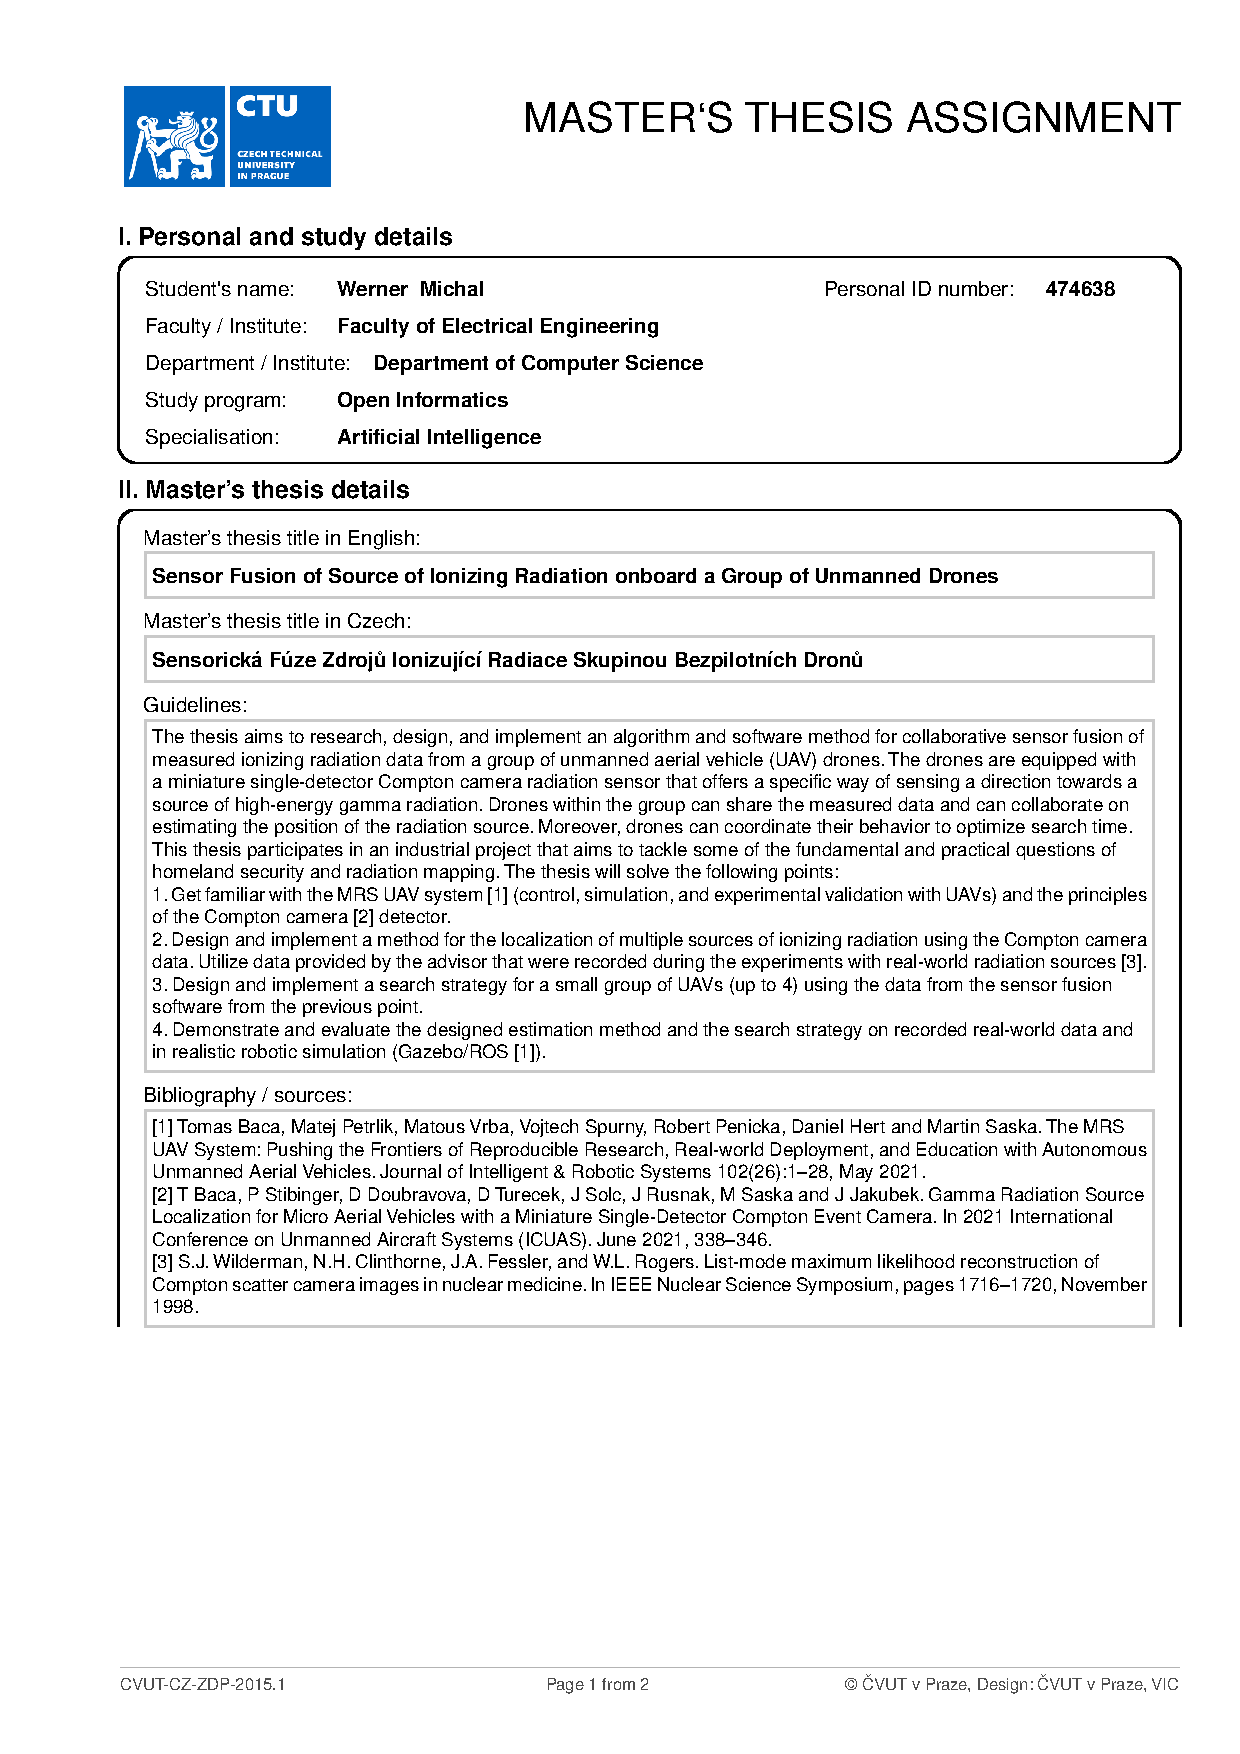
\includepdf[pages=-]{src/assignment.pdf}
%% --------------------------------------------------------------
%% |                          Abstracts                         |
%% --------------------------------------------------------------

%%%%%%%%%%%%%%declaration

\conditionalClearPage

%!TEX root = ../main.tex
\vspace{10cm}

\section*{Declaration}
I declare that presented work was developed independently, and that I have listed all
sources of information used within, in accordance with the methodical instructions for
observing ethical principles in preparation of university theses.

\vspace{2cm}
Prague, date ................... \ \ \ \ \ \ \ \ \ \ \ \ \ \ \ \ \ \ \ \ \ \ \ \ \ \ \ \ \ \ \ \ \ \ \ \ \ \ \ \ \ \ \ \ \ \ \ \ \ \ \ \ \ \ \ \ \ \ \ \ \ \ \ \ ................... 







\conditionalClearPage

%!TEX root = ../main.tex

\begin{changemargin}{0.8cm}{0.8cm}

~\vfill{}

\section*{Abstract}
\vskip 0.5em

This thesis presents a method for localizing multiple sources of ionizing radiation using a group of \acp{UAV}. 
These \acp{UAV} are equipped with miniature single-detector Compton camera radiation sensors, enabling them to estimate the directions towards high-energy gamma radiation sources.
  The proposed radiation mapping method (utilizing a \ac{MLE} principle) fuses the measurements from the Compton camera sensors to accurately estimate the positions of radioactive sources during the flight.
The properties of the used detector are approximated using Monte Carlo simulation techniques.
The estimation method is combined with an active search strategy that coordinates future action of the drones in order to improve the quality of estimate of sources position and minimize search time.
%In addition, an active search strategy is incorporated into the system, coordinating the future actions of the drones. 
%This strategy aims to improve the quality of the estimated source positions and minimize the search time by efficiently exploring the designated area of interest.
The proposed solution is evaluated on recorded real world data and in realistic simulator.





  \mycomment{
%The study of autonomous \acp{UAV} has become a prominent sub-field of mobile robotics.

This thesis presents a method for localization of multiple sources of ionizing radiation using a group of autonomous \acp{UAV} 
that are equipped with a miniature single-detector Compton camera radiation sensor capable of estimating directions towards a source of high-energy gamma radiation.
The proposed radiation mapping method (based on a \ac{MLE} principle) fuses the measurements from the Compton camera sensors and estimates the positions of radioactive sources during the flight.
Properties of the detector are approximated using Monte Carlo simulation.
The estimation method is combined with an active search strategy that coordinates future action of the drones in order to improve the quality of estimate of sources position and minimize search time.
The solution is evaluated on recorded real world data and in realistic simulator.
%The proposed estimation method based on maximum likelihood principle fuses the Compton camera measurements and estimates the positions of radioactive sources during the flight.
%The MiniPIX TPX3 Compton camera is can electronvolt
%The proposed solution utilizes a data fusion method based on \ac{MLEM} algorithm, which combines measurements from multiple \acp{UAV} and estimates the positions of radioactive sources during the flight.
%The fusion method 

%  for fusing the measurements
%and estimating the radiation source position during the flight.
}
\vskip 1em

{\bf Keywords} \Keywords

\vskip 2.5cm

\end{changemargin}


\conditionalClearPage

%!TEX root = ../main.tex

\begin{changemargin}{0.8cm}{0.8cm}

~\vfill{}

\section*{Abstrakt}
\vskip 0.5em

\sloppy
Výzkum na poli autonomních bezpilotních prostředků (UAV) se stal významným oborem mobilní robotiky.

\vskip 1em

{\bf Klíčová slova} \KlicovaSlova

\vskip 2.5cm

\end{changemargin}


%% --------------------------------------------------------------
%% |                        Abbreviations                       |
%% --------------------------------------------------------------

\conditionalClearPage

\begin{changemargin}{0.8cm}{0.8cm}

~\vfill{}

\section*{Abbreviations}

% this will print only the used abbreviations
%!TEX root = ../main.tex

\begin{acronym}
  \acro{API}[API]{Application Programming Interface}
  \acro{CTU}[CTU]{Czech Technical University}
  \acro{DOF}[DOF]{degree-of-freedom}
  \acro{FOV}[FOV]{Field of View}
  \acro{GNSS}[GNSS]{Global Navigation Satellite System}
  \acro{GPS}[GPS]{Global Positioning System}
  \acro{IMU}[IMU]{Inertial Measurement Unit}
  \acro{MLE}[MLE]{Maximum likelihood estimation}  
  \acro{LKF}[LKF]{Linear Kalman Filter}
  \acro{pix}[Minipix3]{MiniPIX TPX3}
  \acro{CS}[CS]{Compton scattering}
  \acro{PE}[PE]{Photoelectric effect}
  \acro{PET}[PET]{Positron emission tomography}
  \acro{SPECT}[SPECT]{Single Photon Emission Computed Tomography}
  \acro{FDNPP}[FDNPP]{Fukushima Daiichi Nuclear Power Plant}
  \acro{LM-MLEM}[LM-MLEM]{List-Mode Maximum Likelihood Expectation Maximization}
  \acro{MLEM}[MLEM]{Maximum Likelihood Expectation Maximization}
  \acro{MAP}[MAP]{Maximum A Posteriori}
  \acro{SOE}[SOE]{Stochastic Origin Ensemble}
  \acro{CC}[CC]{Compton camera}
  \acro{TSP}[TSP]{Travelling salesman problem}
  \acro{MAV}[MAV]{Micro Aerial Vehicle}
  \acro{MPC}[MPC]{Model Predictive Control}
  \acro{MRS}[MRS]{Multi-robot Systems Group}
  \acro{ROS}[ROS]{Robot Operating System}
  \acro{SLAM}[SLAM]{Simultaneous Localization And Mapping}
  \acro{UAV}[UAV]{Unmanned Aerial Vehicle}
  \acro{UGV}[UGV]{Unmanned Ground Vehicle}
\end{acronym}


\vskip 2.5cm

\end{changemargin}

\conditionalClearPage

%% --------------------------------------------------------------
%% |                      Table of contents                     |
%% --------------------------------------------------------------

\tableofcontents

\conditionalClearPage

% set up the full page style with normal page numbering
\pagestyle{full}
\pagenumbering{arabic}

%% --------------------------------------------------------------
%% |                        introduction                        |
%% --------------------------------------------------------------
\acresetall
%!TEX root = ../main.tex

\chapter{Introduction\label{chap:introduction}}

First, introduce the reader to the research topic.
Start with the most general view and slowly converge to the particular field, sub-field, and the challenges you face.
You can cite others' work here \cite{baca2021mrs}.

\section{Related works}

This section should contain related state-of-the-art works and their relation to the author's work.
We usually cite the original works like this \cite{benallegue2008high}.
You can also cite multiple papers at once like this \cite{baca2016embedded, baca2021mrs}.




\subsection{ MRS paper}
This thesis builds on the work of the MRS group (Faculty of Electrical engineering, CTU in Prague) in the field of radiation mapping. 
This paper \cite{baca2021gamma} presents a multi-robotic approach to an autonomous localisation of a compact gamma radiation source. 
All unmanned aerial vehicles are equipped with compact MiniPIX TPX3 CdTe event camera, which is capable of measuring gamma particles and reconstructing Compton events. 
The output of the sensor are Compton cones are used for localisation in the following way:
in the first phase of autonomous exploration, the \ac{UAV}s are exploring the area to measure the first Compton cones. 
After the first eight cones are reconstructed, their intersection is computed using optimisation methods (quadratic programming). 
This initial estimate is then incrementally updated using new measurements. 
The current estimate is always orthogonally projected to the newly measured cone. 
These measurements are fused using \ac{LKF}. 
The \ac{UAV}s are controlled in a way that they encircle the current estimate in order to measure more cones and update the \ac{LKF} estimate.

Using this approach, the group of drones is capable to localise a single compact source of ionising radiation. 
The source can be static or dynamic. 
However, this iterative method cannot localise multiple sources of radiation.
Once the drones detect one source of radioactive particles, they start encircling the current estimate and cannot find other sources in the area.

The main purpose of this thesis is to improve the presented solution: introduce a new method that could localise multiple sources of ionising radiation and control group of \ac{UAV}s to explore the whole area and maximise information gain given the specific sensor.



\section{TODO}
\begin{itemize}
\item clanek MRS ze ktereho vychazim
\item diplomka Petra Štibingera
\item ostatni robotické články týkající se robotickeho pruzkumu, leteckeho nebo pozemniho
\end{itemize}
\section{Contributions}

This section should describe the author's contributions to the field of research.

\section{Mathematical notation}

It is a good practice to define basic mathematical notation in the introduction.
See \reftab{tab:mathematical_notation} for an example.

\begin{table*}[!h]
  \scriptsize
  \centering
  \noindent\rule{\textwidth}{0.5pt}
  \begin{tabular}{lll}
    $\mathbf{x}$, $\bm{\alpha}$ & vector, pseudo-vector, or tuple\\
    $\mathbf{\hat{x}}$, $\bm{\hat{\omega}}$& unit vector or unit pseudo-vector\\
    $\mathbf{\hat{e}}_1, \mathbf{\hat{e}}_2, \mathbf{\hat{e}}_3$ & elements of the \emph{standard basis} \\
    $\mathbf{X}, \bm{\Omega}$ & matrix \\
    $\mathbf{I}$ & identity matrix \\
    $x = \mathbf{a}^\intercal\mathbf{b}$ & inner product of $\mathbf{a}$, $\mathbf{b}$ $\in \mathbb{R}^3$\\
    $\mathbf{x} = \mathbf{a}\times\mathbf{b}$ & cross product of $\mathbf{a}$, $\mathbf{b}$ $\in \mathbb{R}^3$\\
    $\mathbf{x} = \mathbf{a}\circ\mathbf{b}$ & element-wise product of $\mathbf{a}$, $\mathbf{b}$ $\in \mathbb{R}^3$ \\
    $\mathbf{x}_{(n)}$ = $\mathbf{x}^\intercal\mathbf{\hat{e}}_n$ & $\mathrm{n}^{\mathrm{th}}$ vector element (row), $\mathbf{x}, \mathbf{e} \in \mathbb{R}^3$\\
    $\mathbf{X}_{(a,b)}$ & matrix element, (row, column)\\
    $x_{d}$ & $x_d$ is \emph{desired}, a reference\\
    $\dot{x}, \ddot{x}, \dot{\ddot{x}}$, $\ddot{\ddot{x}}$ & ${1^{\mathrm{st}}}$, ${2^{\mathrm{nd}}}$, ${3^{\mathrm{rd}}}$, and ${4^{\mathrm{th}}}$ time derivative of $x$\\
    $x_{[n]}$ & $x$ at the sample $n$ \\
    $\mathbf{A}, \mathbf{B}, \mathbf{x}$ & LTI system matrix, input matrix and input vector\\
    \emph{SO(3)} & 3D special orthogonal group of rotations\\
    \emph{SE(3)} & \emph{SO(3)}~$\times~\mathbb{R}^3$, special Euclidean group\\
  \end{tabular}
  \noindent\rule{\textwidth}{0.5pt}
  \caption{Mathematical notation, nomenclature and notable symbols.}
  \label{tab:mathematical_notation}
\end{table*}


%!TEX root = ../main.tex

\chapter{Preliminaries\label{chap:preliminaries}}

\section{Radioactivity}
Radioactivity is a natural phenomenon in which unstable atomic nuclei undergo spontaneous decay, emitting radiation in the form of particles or electromagnetic waves. 
This process occurs in certain types of atoms, known as radioactive isotopes or radionuclides. 
The radioactive atom aims to achieve a state of stability by dispensing energy in the form of ionizing radiation.
Ionizing radiation refers to any form of radiation with enough energy to remove tightly bound electrons from the orbit of an atom.
Among others, radioactive decay releases three main types of ionizing radiation: alpha, beta and gamma. 

\section{Some properties of ionizing radiation}

\subsection{Health risks}% %%{
Several health risks are associated with ionizing radiation.
While traversing the human body, ionizing radiation can interact with living tissues causing damage or mutations of individual cells.
In the long-term horizon, exposure to ionizing radiation might cause cancer or even genetic disorders.
The severity of health problems depends on the exposure time and dose of absorbed radiation.
High doses of ionizing radiation over a short period can cause acute radiation syndrome (radiation sickness).
The disease is manifested by nausea, vomiting, fatigue or even skin burns. 
Depending on the absorbed radioactive dose, it causes several neurological or cardiovascular problems or might lead to death.% %%}

\subsection{Activity}% %%{
``Activity'' is one of the terms used to quantify and describe the properties of radioactive sources.
It is defined as the number of radioactive decays per second.
The unit of activity is called Becquerel ($\si{\becquerel}$) and belongs to SI\footnote{International System of units} units.
In other words, if a radioactive source has activity one Becquerel, it means that one unstable nucleus decays per second (on average, since the decay is a stochastic process).
It is important to note that the Becquerel only measures the rate of decay and does not take into account the type or energy of the radiation involved.% %%}
However, for the purpose of this thesis, ``activity''  is used as the number of gamma photons emitted from the source position in any direction per second.

\subsection{Inverse square law}% %%{
The inverse square law is a fundamental principle that applies to diverse physical phenomena, including radiation.
It describes how the intensity of radiation decreases with increasing distance from the source.
The intensity of radiation is inversely proportional to the square distance from the source:
\begin{equation}
  intensity \approx \frac{1}{distance^2}.
\end{equation}
For example, doubling the distance to the source means that the intensity decreases to $\frac{1}{4}$.
As illustrated in figure \ref{fig:islaw}, this principle comes from the fact that the radiation spreads out over a larger area when the observer is further away from the source.
This rapid decrease makes the search for sources of ionizing radiation challenging since it limits the sensing range of the detectors.

  \begin{figure}[!h]
    \centering
      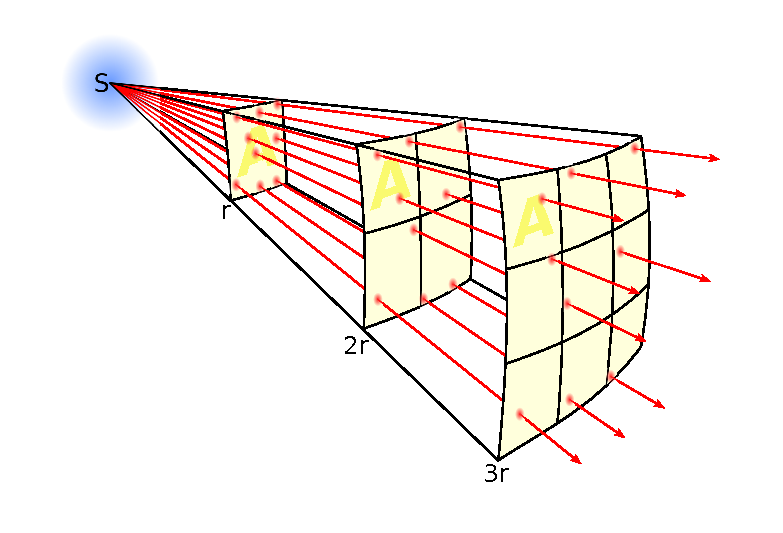
\includegraphics[width=0.65\textwidth]{./fig/photos/Inverse_square_law.eps}
    \caption{An illustration of the inverse square law for the intensity of radiation. Source: \cite{inverse_square_law}}
      \label{fig:islaw}
  \end{figure}

% %%}
\section{Main types of ionizing radiation}
\subsection{Alpha radiation}
Alpha radiation is an emission of positively charged alpha particles consisting of two protons and two neutrons bound together (helium nuclei).
This gives alpha particles a significantly larger mass and higher reactivity compared to other types of ionizing radiation.
On the other hand, they interact strongly with matter and can't penetrate far.
Alpha particles can travel only a few centimetres in the air and can be blocked by a single sheet of paper or the outer layer of human skin.
Because of that, external sources of alpha radiation are generally not considered a significant threat to human health.
The limited range of alpha radiation makes it difficult to sense from a distance.

\subsection{Beta radiation}
Beta particles are high-energy, high-speed electrons or positrons.
Due to their smaller size and weaker electrical charge, they are generally more penetrating and less reactive than alpha particles and can reach further into materials.
Several centimetres thick sheet of aluminium or plastic is typically sufficient to block the beta radiation.
In terms of travel through the air, beta particles have a range of a few meters.
Although beta radiation is generally less dangerous than gamma, when particles come into contact with human skin, they can penetrate the outer layers and cause skin burns as the particles disrupt cellular processes.

\subsection{Gamma radiation}
Gamma particles are often produced alongside alpha or beta particles during radioactive decay. 
Unlike them, gamma radiation of composed of high-energy photons. 
They are extremely penetrating and can travel long distances in the air and get through most of materials or living tissues thanks to their high energy and lack of charge.
Only a thick layer of concrete or lead might block this type of ionizing radiation.
These features make gamma radiation significantly more dangerous than alpha and beta.
The long-range of gamma radiation, together with its negative effects on human health, makes it an ideal candidate for remote sensing and detection.
  \begin{figure}[!h]
    \centering
      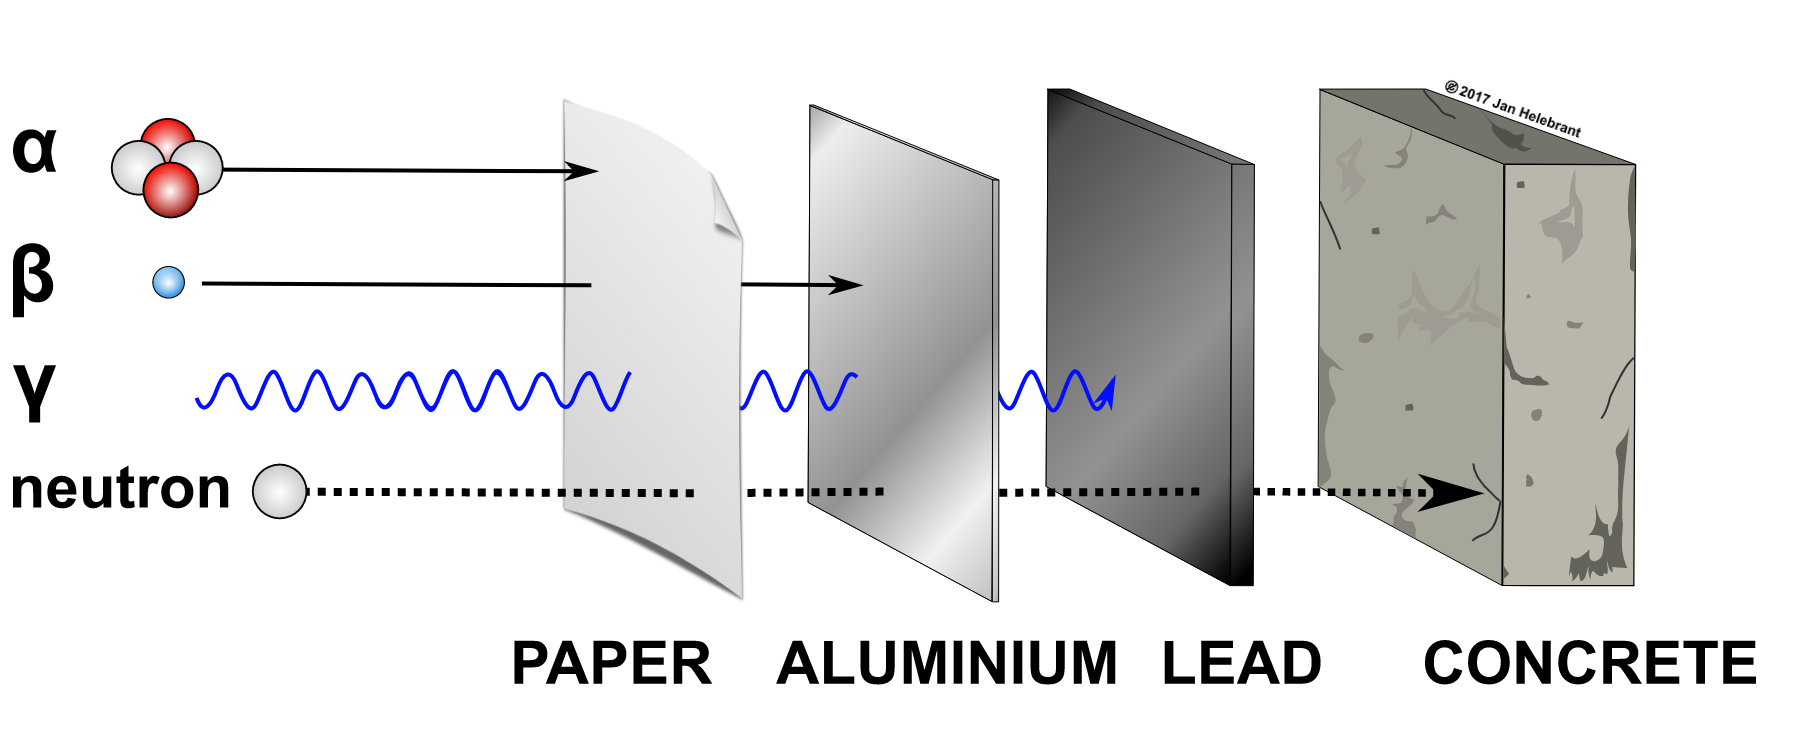
\includegraphics[width=0.6\textwidth]{./fig/photos/pene2.png}
    \caption{Penetrating power of different types of radiation. Source: \cite{penetrating_power}}
      %\label{fig:islaw}
  \end{figure}

\subsubsection{Cesium-137}
Cesium-137 is a radioactive isotope of cesium and one of the most common bi-products of nuclear fission.
It is used in radiotherapy in medicine, for calibration of radiation detection equipment in the industry and 
(most importantly) it is one of the most common fission products by the nuclear fission of uranium-235, which is used as a fuel in nuclear power plants and in nuclear weapons.
Cesium-137 is also the main source of radioactive pollution caused by accidents in Chornobyl (1986) and Fukushima (2011).
The half-life (defined as the interval of time required for one-half of the atomic nuclei of a radioactive sample to decay) of cesium-137 is $30.05$ years.
It is important to note that cesium-137 itself is not a source of $\gamma$ radiation.
However, it decays by beta emission to metastable Barium-137, which decays almost immediately (with a half-life of about $2.5$ minutes) and emits $\gamma$ photons with initial energy $\SI{662}{\kilo\electronvolt}$.
Cesium-137 (with its long half-life, negative health effects, wide usage and high penetrating power of $\SI{662}{\kilo\electronvolt}$ photons) is a good candidate for remote sensing. 
The methods proposed in this thesis have been tested using Cesium-137 radioactive isotope as a source of radiation (during simulated and real-world experiments).

\section{Interaction of $\gamma$ radiation with matter}
Sensing of $\gamma$ radiation is possible through interactions of ionizing photons with imaging devices.
%A variety of interactions may take place as a high-energy photon travels through matter.
Several interactions might occur when a high energetic photon travels through matter.
Type of the interaction depends on both the energy of the incoming photon and the properties of the material it encounters. 
%epending on the energy of the incoming photon as well as on the properties of material.
%Three main types of interactions are: a photoelectric effect, Compton scattering and pair production.
The three primary types of interactions include the photoelectric effect, Compton scattering, and photon-electron pair production.
Figure \ref{fig:dominant} describes the dominant type of interactions depending on the energy of the incoming photon and the atomic number of the material.

\subsection{Photoelectric effect and pair production}
In \ac{PE}, alternatively referred to as photoelectric absorption, the $\gamma$ photon interacts with an orbital electron of the absorbing atom.
The photon transfers all its energy to the electron and disappears.
As a consequence, the electron exceeds its binning energy and is emitted from the atom.
Photoelectric absorption is dominant at lower energies of the incident photon, although it can occur at any photon energy.
The \ac{PP} occurs only if the $\gamma$ photon has energy exceeding $\approx \SI{1}{\mega\electronvolt}$.
In this case, the highly energetic photon interacts with the atom's nucleus. 
The interaction results in the creation of an electron-positron pair.

\begin{figure}[!h]
  \centering 

    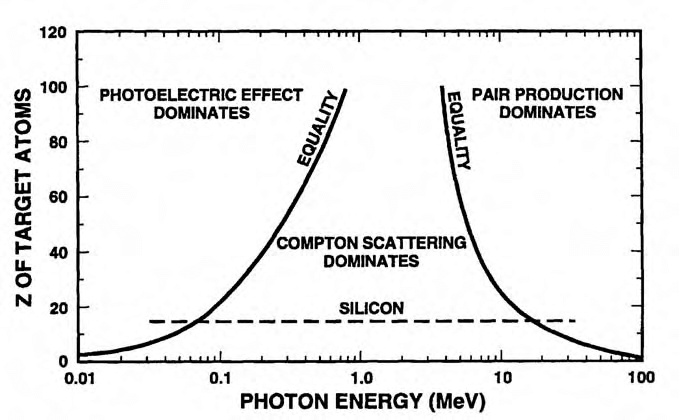
\includegraphics[width=0.6\textwidth]{./fig/photos/dominant.png}
  \caption{Dominant types of interactions for different energy of photon (x-axis) and atomic number of material (y-axis). Source of image: \cite{schwank}}
    \label{fig:dominant}
  
\end{figure}

\subsection{Compton scattering}
The third potential interaction, primarily prevalent at mid-level energies, is Compton scattering.
In this process, the $\gamma$ photon interacts with an electron that is loosely attached to the nucleus. 
The photon, with its initial energy $E_{0}$, transfers a portion of its energy to the electron.
As a result of the interaction, the lower energetic photon with energy $E_{2}$ is scattered and emitted in a direction changed by angle $\beta$. 
The energy difference $E_{1} = E_{0} - E_{2}$ is transferred to a bi-product of the interaction --- an electron.
The situation is illustrated in figure \ref{fig:scattering}.
According to Compton \cite{compton}, the relation of particle energies and scattering angle $\beta$ can be expressed as:
\begin{equation}
E_{2} = \frac{E_{0}}{  1 + (E_{0} / m_{e}c^{2}) (1 - \mathrm{cos} \beta)},
  \label{eq:compton_energies}
\end{equation}
where $E_{0}$ is the initial energy of the incoming photon, $E_{2}$ is the energy of scattered photon,  $m_{e}$ is the electron rest mass and $c$ is the speed of light in vacuum. 
\begin{figure}[!h]
    \centering
    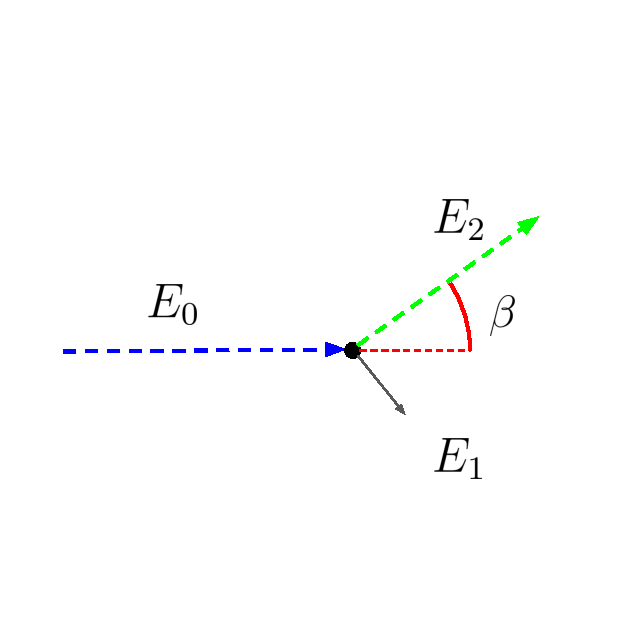
\includegraphics[width=0.4\textwidth]{./fig/photos/compton_simple2.eps}
    \caption{An illustration of the Compton scattering. The incident $\gamma$ photon with energy $E_{0}$ (blue) undergoes the Compton scattering. As a result of the interaction, the lower energetic photon (green) with energy $E_{2}$ is emitted under angle $\beta$. Part of the energy ($E_{1}$) is transferred to a bi-product of the interaction- the electron (grey).}
    \label{fig:scattering}
\end{figure}

\mycomment{ %klein nishina % %%{
  The probability that a photon with an energy $E_{0}$ undergoes a Compton scattering through an angle $\beta$ is described by the Klein-Nishina formula
  \begin{equation}
    K(\beta, E_{0}) = \frac{r_{e}^{2}}{2} \left( \frac{E_{2}}{E_{0}}  \right)^{2} \left(  \frac{E_{2}}{E_{0}} + \frac{E_{0}}{E_{2}} - \mathrm{sin}^{2}(\beta)  \right),
    \label{eq:klein_nishina}
  \end{equation}
  where $r_{e}$ is the classical electron radius. 
}% %%}

\mycomment{% %%{
  \section{Measuring radioactivity}
  Ionizing radiation is unperceivable by human senses yet poses a significant health risk for human beings.
  Effective monitoring methods are therefore needed to detect and measure the presence of such radiation. %, that is potentially harmful to human beings.
  %Sensors of ionizing radiation are made of different materials that interact with ionizing particles.
  Therefore, efficient methods for monitoring and detecting this type of radiation are essential. 
  Various materials that interact with ionizing particles are used to construct sensors for ionizing radiation.

  Three common types of these sensors include Geiger-Müller counters, scintillation detectors, and semiconductor detectors (among many others).
   Geiger-Müller counters are tubes filled with gas that, when ionized by passing particles, conduct an electrical charge proportional to the detected particle flux.
  Scintillation detectors work differently. 
  They contain a material that emits light when hit by ionizing radiation, 
  which is then transformed into an electrical signal by a photodiode. 
  The third type of detector is made from semiconductive materials sensitive to ionizing photons. 
  The ejected electrons from the ionization process can be measured to deduce the type and energy of the incoming radiation.

  Most of these sensors function by counting the number of particles detected, thus estimating the intensity of the particle flux at the sensor's location. 
  However, this does not provide information about the direction from which the particles are coming. 
  Following \cite{baca2019timepix}, the direction of incoming particles can be deduced by different detector configurations illustrated in figure \ref{fig:sensor_overview}.
  \textbf{Pinhole camera aperture} (which is based on same principles as pinhole camera in classical optics) consists of a small hole in shielding material (e.g. lead), blocking all rays in other directions.
  This approach significantly reduces the field of view of the camera. 
  \textbf{Colimators} (frequently used in medical imaging) also restrict the set of possible directions.
  The openings in the shielding material are organized in a way that each part of the detector is responsible for measuring particles coming from certain direction.
  \textbf{Stacked detectors} employ multiple layers of detectors, where the particle's direction is computed from multiple interactions as the ray passes through the layers.
  Finally, the \textbf{Compton camera} use the Compton scattering for deducing the set of possible directions of the original particle. 



  %Each of the proposed methods have some drawbacks in context of deployment onboard a small \ac{UAV}.
  Intensity-only detectors must be relative large to get accurate measurements (collect enough interactions and compensate the stochastic nature of radioactive decay).  
  Moreover, localization of multiple sources might require many measurements at different positions, which is time consuming.
  The use of collimators or pin-hole apertures is not possible due to their limited field of view and large weight and dimensions (caused by the presence of shielding material, which must be thick enough to effectively block the other rays).
  Multi-stack detectors are complicated 
  \begin{figure}[!h]
      \centering
      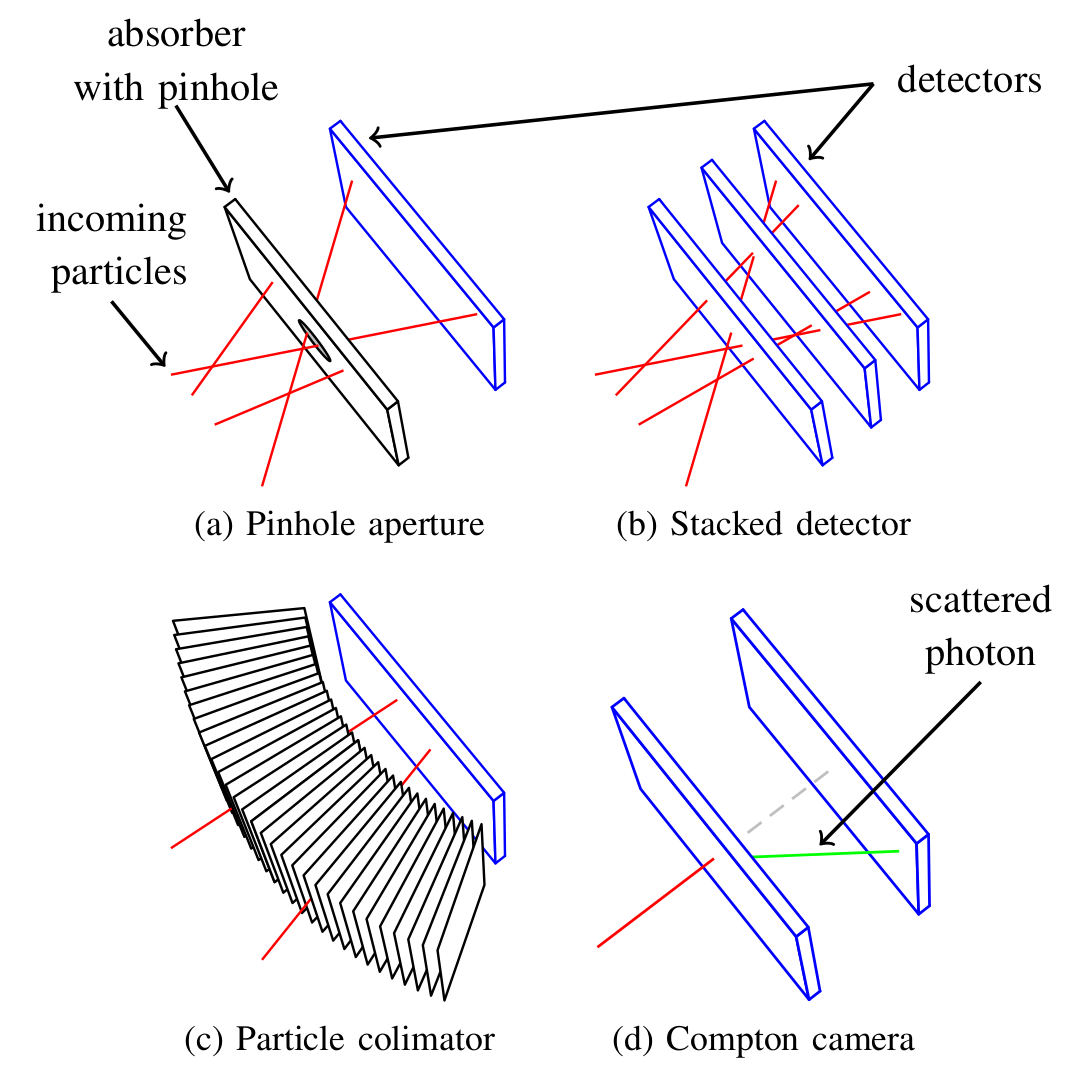
\includegraphics[width=0.5\textwidth]{./fig/photos/detector_overview_baca2019.png}
      \caption{Different ways how to deduce the direction of the incoming particle. Source: \cite{baca2019timepix}}
      \label{fig:sensor_overview}
  \end{figure}
}% %%}

\mycomment{% %%{
\begin{figure}[!h]% %%{
  \centering
  \subfloat[\centering different ways how to detect the direction of incoming particle. Source: \cite{baca2019timepix}] {
    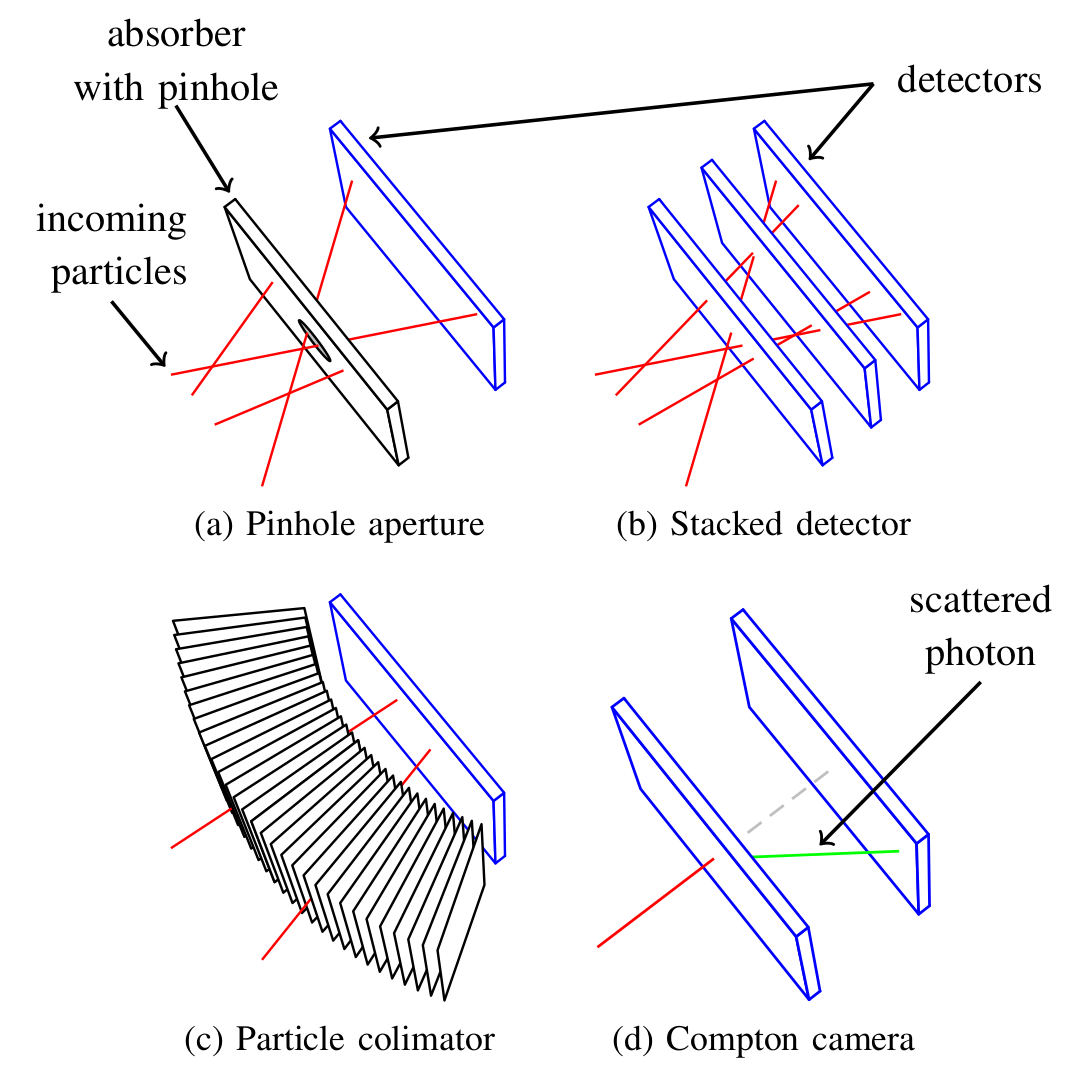
\includegraphics[width=0.49\textwidth]{./fig/photos/detector_overview_baca2019.png}
    \label{fig:sensor_overview}
  }
  \subfloat[\centering Geometry for two-layer Compton camera. The $\gamma$ particle emitted at position $j$ interacts with the first layer of the sensor (scatterer) at position $X_{1}$. A lower energetic photon is scattered under angle $\beta$ and absorbed by the second layer of the detector (absorber) at position $X_{2}$. The reconstructed Compton cone is parametrized by angle $\beta$, axis vector $a$ and origin of the cone $X_{1}$.] {
      \label{fig:compton_camera_geometry}
  
      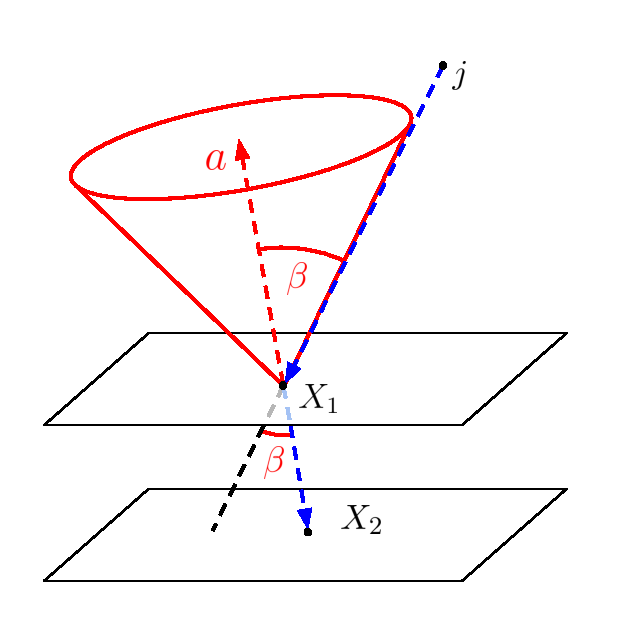
\includegraphics[width=0.49\textwidth]{./fig/photos/compton_camera_modelll.eps}
  }
  \caption{TODO}
  \label{fig:xxx}
\end{figure}% %%}
}% %%}

%%%%%%%%%%%%%%%%%%%%%%%%%%%%%%%%%%%%%%%
\section{Measuring the gamma radiation}
Ionizing radiation is unperceivable by human senses yet poses a significant health risk for human beings. 
Therefore, efficient methods for monitoring and detecting this type of radiation are essential. 
%Various materials that interact with ionizing particles are used to construct sensors for ionizing radiation.
The primary operating mode of most sensors of radioactivity is counting the number of particles detected,
thus estimating the intensity of the particle flux at the sensor's location. 
However, the dosimetric measurements do not provide information about the direction from which the radiation is emitted. 
Intensity-only detectors must be relatively large to get accurate measurements (must collect enough interactions and compensate for the stochastic nature of radioactive decay).
Moreover, the localization of multiple sources might require many measurements at different positions, which is time-consuming. 
The direction of incoming $\gamma$ photons might be deduced using
the Compton camera, which is based on the Compton scattering principle.

\mycomment{% %%{
Ionizing radiation is unperceivable by human senses yet poses a significant health risk for human beings.
%Sensors of ionizing radiation are made of different materials that interact with ionizing particles.
Therefore, efficient methods for monitoring and detecting this type of radiation are essential. 
Various materials that interact with ionizing particles are used to construct sensors for ionizing radiation.

The basic operation mode of these sensors is counting the number of particles detected, thus estimating the intensity of the particle flux at the sensor's location.
The dosimetric measurements do not provide information about the direction from which direction the radiation is emitted. 
Intensity-only detectors must be relative large to get accurate measurements (must collect enough interactions and compensate the stochastic nature of radioactive decay).  
Moreover, localization of multiple sources might require many measurements at different positions, which is time consuming.
The direction of incoming $\gamma$ photons might be deduced using the Compton camera, which is based on the Compton scattering principle.
}% %%}
\mycomment{% %%{
  %The 
  Geiger-Müller counters, scintillation detectors, and semiconductor detectors (among many others).
   Geiger-Müller counter a tube filled with gas that, when ionized by passing particles, conducts an electrical charge corresponding to the detected particle flux.
  Scintillation contains a luminescent material that emits light when hit by ionizing radiation, 
  which is then transformed into an electrical signal by a photodiode. 
  The third common type of detector is made from semiconductive materials sensitive to ionizing radiation. 
  The ejected electrons from the ionization process can be measured to deduce the type and energy of the incoming radiation.
}% %%}
\subsection{Compton Camera}% %%{
The Compton camera is typically composed of two detectors: a scatterer and an absorber.
The incident photon with energy $E_{0}$ first interacts with the scatterer at position $X_{1}$ in the form of Compton scattering.
A bi-product of the interaction (electron with energy $E_{1}$) is immediately captured by the scatterer, and its position $X_{1}$ and energy are recorded.
As a result of the interaction, a lower energetic photon with energy $E_{2}$ is scattered under (Compton) angle $\beta$.
The scattered photon then interacts in the form of \ac{PE} with the absorber.
The absorbed energy $E_{2}$ and the position of the interaction $X_{2}$ are measured and recorded.

The scattering angle $\beta$ can be reconstructed (following \cite{baca2021gamma}) from equation \ref{eq:compton_energies} as:
\begin{equation}
  %\beta = \mathrm{arccos} \left (  1-\frac{m_{e}c^{2}E_{2}}{E_{0} (E_{0} - E_{2})} \right )
  \beta = \mathrm{cos}^{-1} 
  \underset{B}{\underbrace{\left (
   1+m_{e}c^{2} \left( \frac{1}{E_{1}+E_{0}} - \frac{1}{E_{0}}\right )  \right )
  }},
    \label{eq:compton_beta_formula}
\end{equation}
assuming that $0<B<1$.
Since Compton scattering is a symmetrical phenomenon,  the set of possible directions of incoming particles forms a surface of a cone.
Such conical surface (denoted as Compton cone) is parametrized by the cone axis $\mathbf{a}$ (which is a straight line connecting the positions of intersections $X_{1}$ and $X_{2}$), Compton scattering angle $\beta$ and origin of the cone $X_{1}$.
The geometry is illustrated in figure \ref{fig:compton_camera_geometry}.

\begin{figure}[!h]
  \centering
    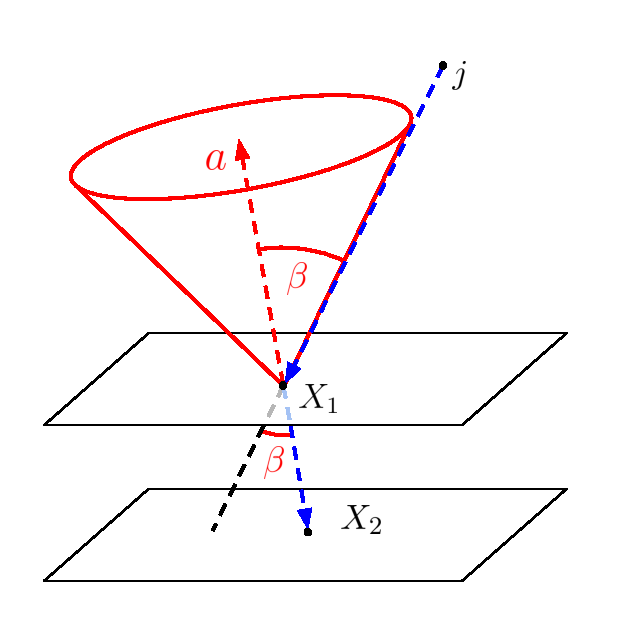
\includegraphics[width=0.4\textwidth]{./fig/photos/compton_camera_modelll.eps}
    \caption{Geometry for two-layer Compton camera. The $\gamma$ particle (emitted at position $j$) interacts with the first layer of the sensor (the scatterer) at position $X_{1}$. A lower energetic photon is scattered under angle $\beta$ and absorbed by the second layer of the detector (absorber) at position $X_{2}$. The reconstructed Compton cone is parametrized by angle $\beta$, axis vector $a$ and origin of the cone $X_{1}$.}
    \label{fig:compton_camera_geometry}
\end{figure}
% %%}
\subsection{The MiniPIX TPX3 sensor} % %%{
The MiniPIX TPX3 detector\footnote{produced by \textit{Advacam}, https://advacam.com/camera/minipix-tpx3} (in the rest of this thesis denoted as \ac{pix}) belongs to the class of semiconductor-based radiation sensors.
The \ac{pix} is composed of a) miniature version Timepix3 pixel detector \cite{timepix3},
b) the body of the sensor made of a compact block of Cadmium telluride (CdTe) semiconductor material (with dimensions $14 \times 14 \times 2 \ \si{\milli\meter}$) 
and c) necessary electronics.
The whole \ac{pix} device is very compact and lightweight (the size of the whole \ac{pix} sensor is only $80 \times 21 \times 14 \ \si{\milli\meter}$ and it weights $\SI{44}{\gram}$), therefore it can be carried onboard a small \ac{UAV}.
Unlike other devices, the \ac{pix} sensor can report the recorded $\gamma$ particles almost in real-time, which allows us to use it for an active strategy, where autonomous \ac{UAV}s react according to the measurements acquired during the flight.

Although \ac{pix} has only one detection layer, it can still be used as a Compton camera.
As described in \cite{baca2021gamma} and \cite{baca2019timepix}, the incoming ionizing radiation interacts with the matter of the sensor and separates electrons from the CdTe material.
The separated electrons are accelerated by a $\SI{450}{\volt}$ electric potential towards one facet of the sensor, where the Timepix3 pixel detector is located.
The resolution of pixel detector is $256 \times 256\ \mathrm{px}$, each pixel being $55\ \si{\micro\meter}$ large.
The pixel detector can estimate the energy of the absorbed particle and record the time when it was taken with high resolution.
Given the measured times of arrival, the coinciding products of Compton scattering might be paired together (assuming that both Compton scattering as well as follow-up photon absorption happened at the same time).

Figure \ref{fig:minipix} depicts the geometry of the \ac{pix} sensor and the detection process.
The x-axis and y-axis coordinates (see figure \ref{fig:minipix}) of the interaction are determined by the position of corresponding pixels.
The z-axis coordinate (the depth of interaction in the CdTe block) is unknown.
However, the relative z-axis distance of the two coinciding events might be deduced from the times of arrival of the two interactions captured by the pixel detector (given the known speed of electrons in the CdTe material).
The absolute z-axis coordinate is not needed since the size of the CdTe block is negligible in the context of the detection task.
More technical details related to the sensor operation are provided in \cite{baca2019timepix}.
%The \ac{pix} detector is very compact and lightweight (the size of the whole \ac{pix} sensor is only $80 \times 21 \times 14 \ \si{\milli\meter}$ and it weights $\SI{44}{\gram}$), therefore it can be carried onboard a small \ac{UAV}.
%The \ac{pix} detector can report the recorded intersections almost in real time, which allows us to use it for an active strategy, where autonomous \ac{UAV}s react according to the measurements acquired during the flight.

\begin{figure}[!h]
    \centering
  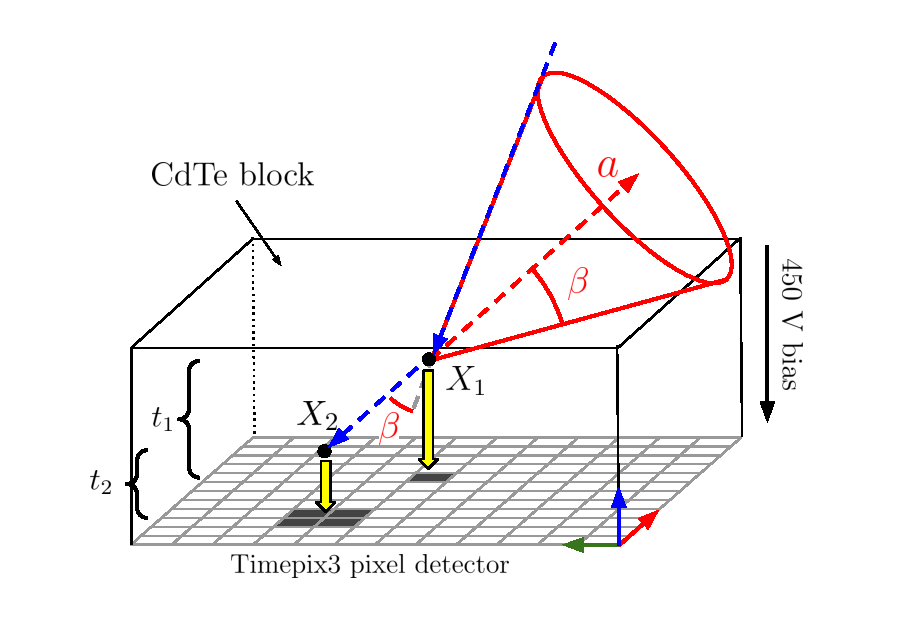
\includegraphics[width=0.7\textwidth]{./fig/photos/my_minipix.eps}
    \caption{An illustration of the detection process inside the \ac{pix} sensor. 
    The incident photon (blue) scatters under angle $\beta$ at position $X_{1}$. 
    The bi-product of the interaction (electron) is immediately absorbed. 
    Scattered photon undergoes photoelectric absorption at position $X_{2}$. 
    The free electrons (produced by the electron's absorption and scattered photon's absorption) are detected by the Timepix3 pixel detector. 2D positions ($\hat{c}_{x}, \hat{c}_{y}$) and energies ($E_{1}, E_{2}$) are recorded. 
    The relative z-axis distance between $X_{1}$ and $X_{2}$ is deduced from the time difference $t_{2}-t_{1}$ and the known speed of electrons in the CdTe block.
    The Compton cone (red) is then reconstructed.}
    \label{fig:minipix}
\end{figure}

\begin{figure}[!h]% %%{
  \centering
  \subfloat[\centering The real size of \ac{pix} sensor. Source: \cite{baca2021gamma} ] {
    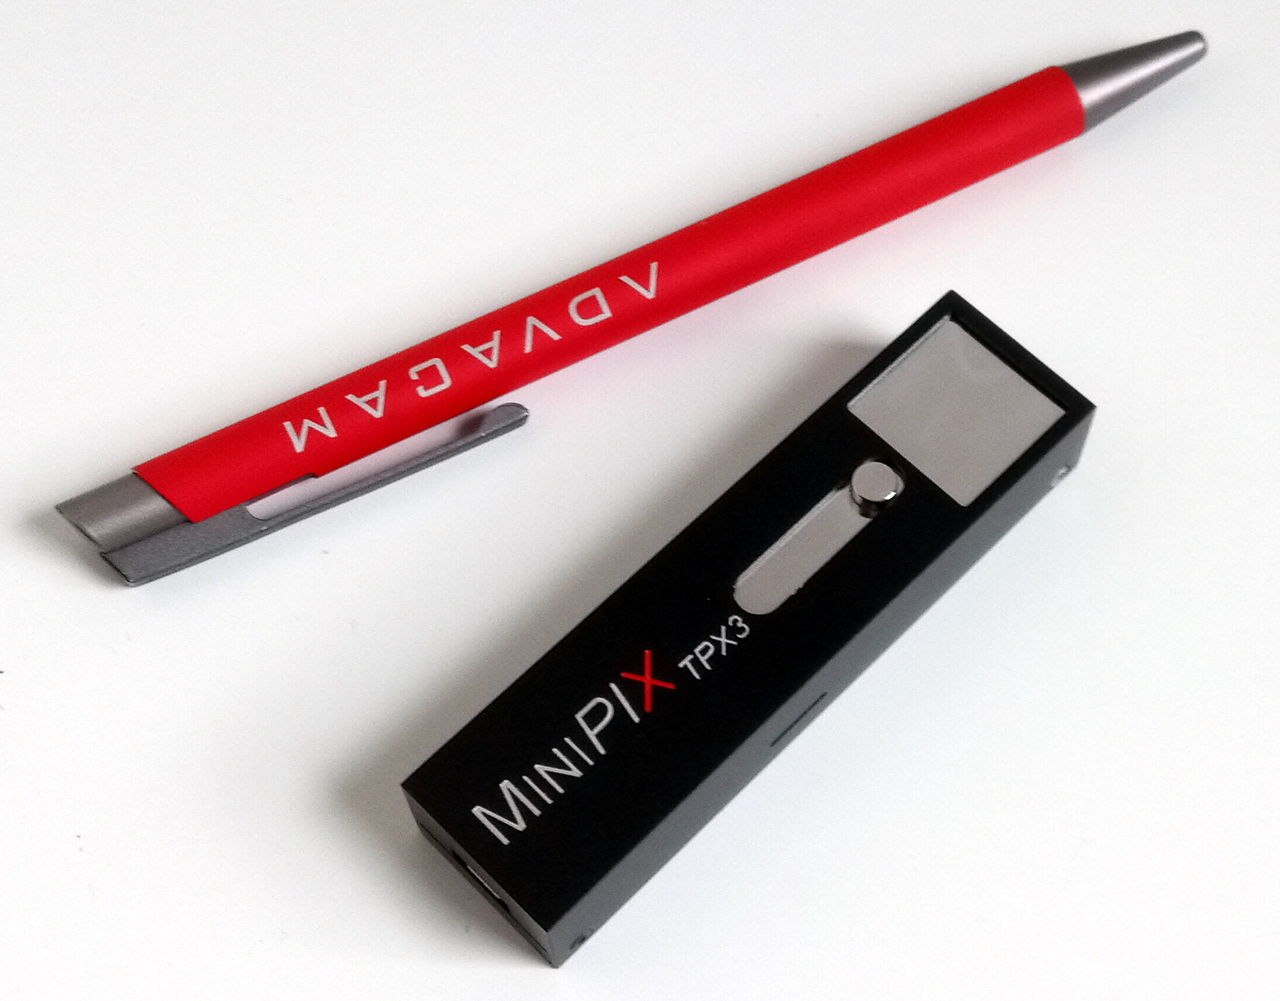
\includegraphics[width=0.35\textwidth]{./fig/photos/minipix_pen.jpg}
    \label{fig:minipix_pen}
  }
  \subfloat[\centering Pixel output of the Timepix3 detector with recorded pair of coinciding events and computed parameters of the Compton cone. Source: \cite{baca2021gamma}] {

    \begin{tikzpicture}
      \node[anchor=south west,inner sep=0] (a) at (0,0) {
          \begin{tabular}{cc}
              \fbox{
\includegraphics[width=0.25\textwidth]{./fig/rviz/timepix_10s.png}}
            &
              \fbox{
\includegraphics[width=0.25\textwidth]{./fig/rviz/timepix_10s_compton_zoom.png}}
          \end{tabular}
        };

      %%{ labels

      \begin{scope}[x={(a.south east)},y={(a.north west)}]

        \draw (0.37, 0.11) rectangle (0.43, 0.20);
        \draw[black] (0.43, 0.11) -- (0.525, 0.005);
        \draw[black] (0.43, 0.20) -- (0.525, 0.995);

        \draw (0.66,0.80) node [text=black] {\small photon track};
        \draw (0.83,0.95) node [text=black] {\small electron track};

        \draw (0.75,0.36) node [text=black] {
          \begin{tabular}{rl}
            \small $E_{1}$ = &\SI{394.22}{\kilo\electronvolt}\\
            \small $E_{2}$ = &\SI{315.70}{\kilo\electronvolt}\\
            \small $t_{2} - t_{1}$ = &\SI{20.31}{\nano\second}\\
            \small $\Delta z$ = &\SI{0.47}{\milli\meter}\\
            \hline
            \small $\beta$ = &\SI{1.13}{\radian}\\
          \end{tabular}
        };

      \end{scope}

      %%}
    \end{tikzpicture}
  %\caption{An example of a pair of Compton scattering products captured by the Timepix3 detector. The event's times are used together with the particle's energies to reconstruct the scattering angle, $\Theta$.
  \label{fig:timepix_image}





  }
  \label{fig:minipix_ilu}
  \caption{The \ac{pix} sensor and it's real size (\ref{fig:minipix_pen}) and the illustration of output from Timepix3 pixel detector (\ref{fig:timepix_image}).} 

\end{figure}% %%}

\mycomment{% %%{
\begin{figure}[!h]
    \centering
  \includegraphics[width=0.2\textwidth]{./fig/photos/minipix_in_hand.png}
    \caption{MiniPIX TPX3 sensor. Source: \url{http://mrs.felk.cvut.cz/rospix3}}
    %\label{fig:minipix}
\end{figure}
}% %%}

\mycomment{% %%{
\begin{figure}[!h]
    \centering
    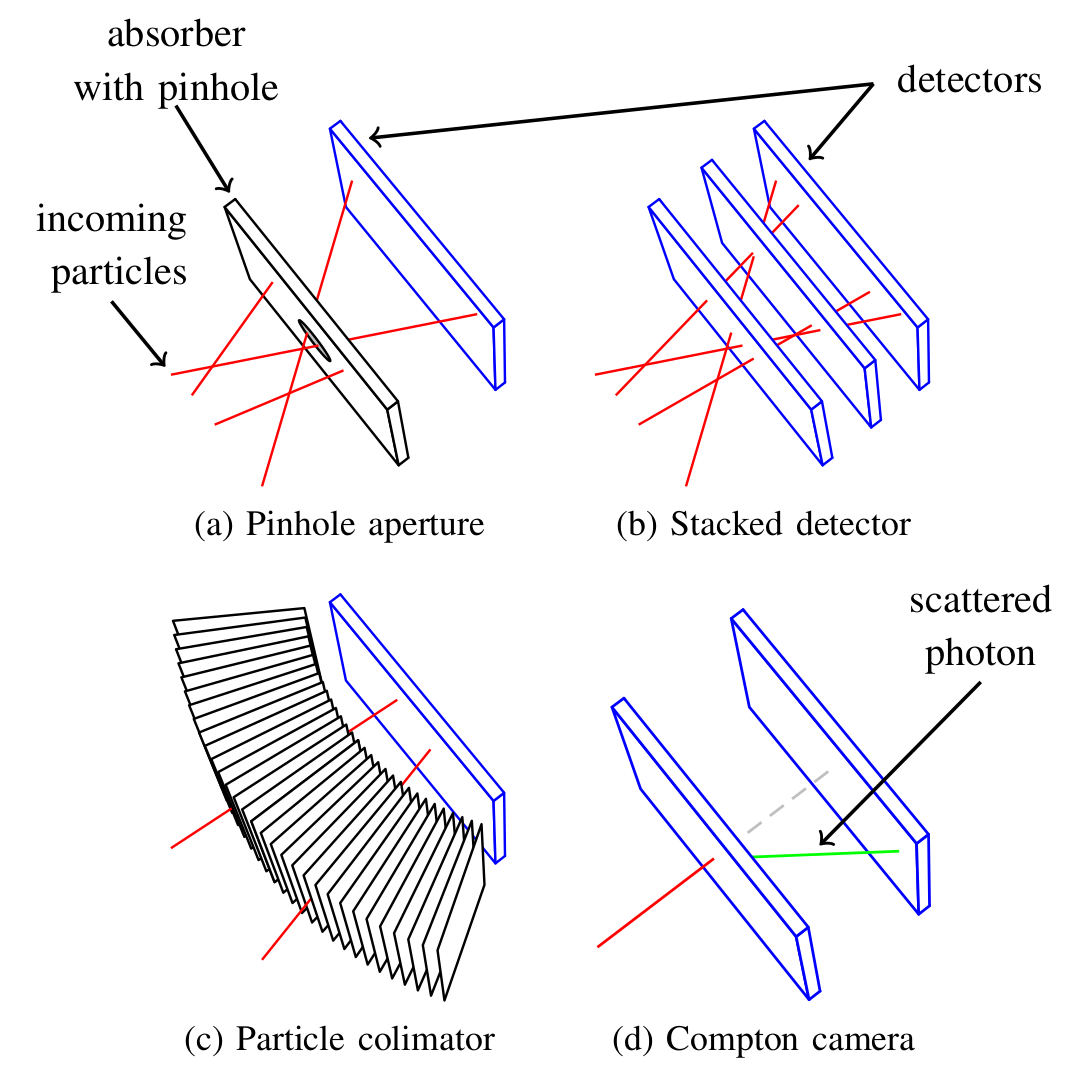
\includegraphics[width=0.5\textwidth]{./fig/photos/detector_overview_baca2019.png}
    \caption{different ways how to detect the direction of incoming particle. Source: \cite{baca2019timepix}}
    \label{fig:sensor_overview}
\end{figure}
}% %%}
% %%}

\section{Robot operating system}
The \ac{ROS} \cite{ROS} is a middleware open-source software framework for robotics applications and research.
\ac{ROS} supports for multiple programming languages, most notably \textit{Python} and \textit{C++}.
Individual software modules (called \textit{nodes}) can exchange data through a standardized communication model.
The registration of the individual \textit{nodes}, as well as communication between them, is maintained by a central authority called \ac{ROS} \textit{master}.
The main advantage of \ac{ROS} is its flexibility - multiple \textit{nodes} might be executed independently without restarting the whole program.
\ac{ROS} provides a variety of other useful tools.
\textit{TF library} keeps track of multiple coordinate frames over time and provides transformations between them.
\textit{Rosbag} is a tool for recording and playing back data collected during the experiments.
\textit{RViz} is helpful 3D graphical interface for visualisation and debugging.
%The key feature of \ac{ROS} is the \textit{transformation} library, which provides transformations between different coordinate frames of the robotic system.
%The \ac{ROS} master provides the registration of the individual \ac{ROS} nodes as well as maintains communication between them.

\subsubsection{ROS communication model}
The fundamental \ac{ROS} communication mechanism used for exchanging messages between different \ac{ROS} \textit{nodes} is called \textit{topics}.
\textit{Topics} are based on a publish-subscribe model, where nodes can either publish data to a topic or subscribe to receive data from a topic. 
Each topic has a specific data type associated with it.
Nodes can publish messages of that data type to the topic, and any subscribed nodes will receive those messages.
Topics enable asynchronous communication between different parts of the robotic system, such as data exchange between sensors and onboard computer.

Another important \ac{ROS} communication concept is called \textit{service}.
\ac{ROS} \textit{services} allow \textit{nodes} to make requests and receive responses to them.
Unlike in \ac{ROS} \textit{topics}, services provide a synchronous request-response communication model.
The client node sends its request to a specific service provided by the server node.
The server node processes the request and generates a response message, which is sent back to the sender.
Such a communication scheme might be used, for example, for triggering some action, requesting a path from the planning node and generally in any situation where a response from the server node is required.

\begin{figure}[!h]
    \centering
  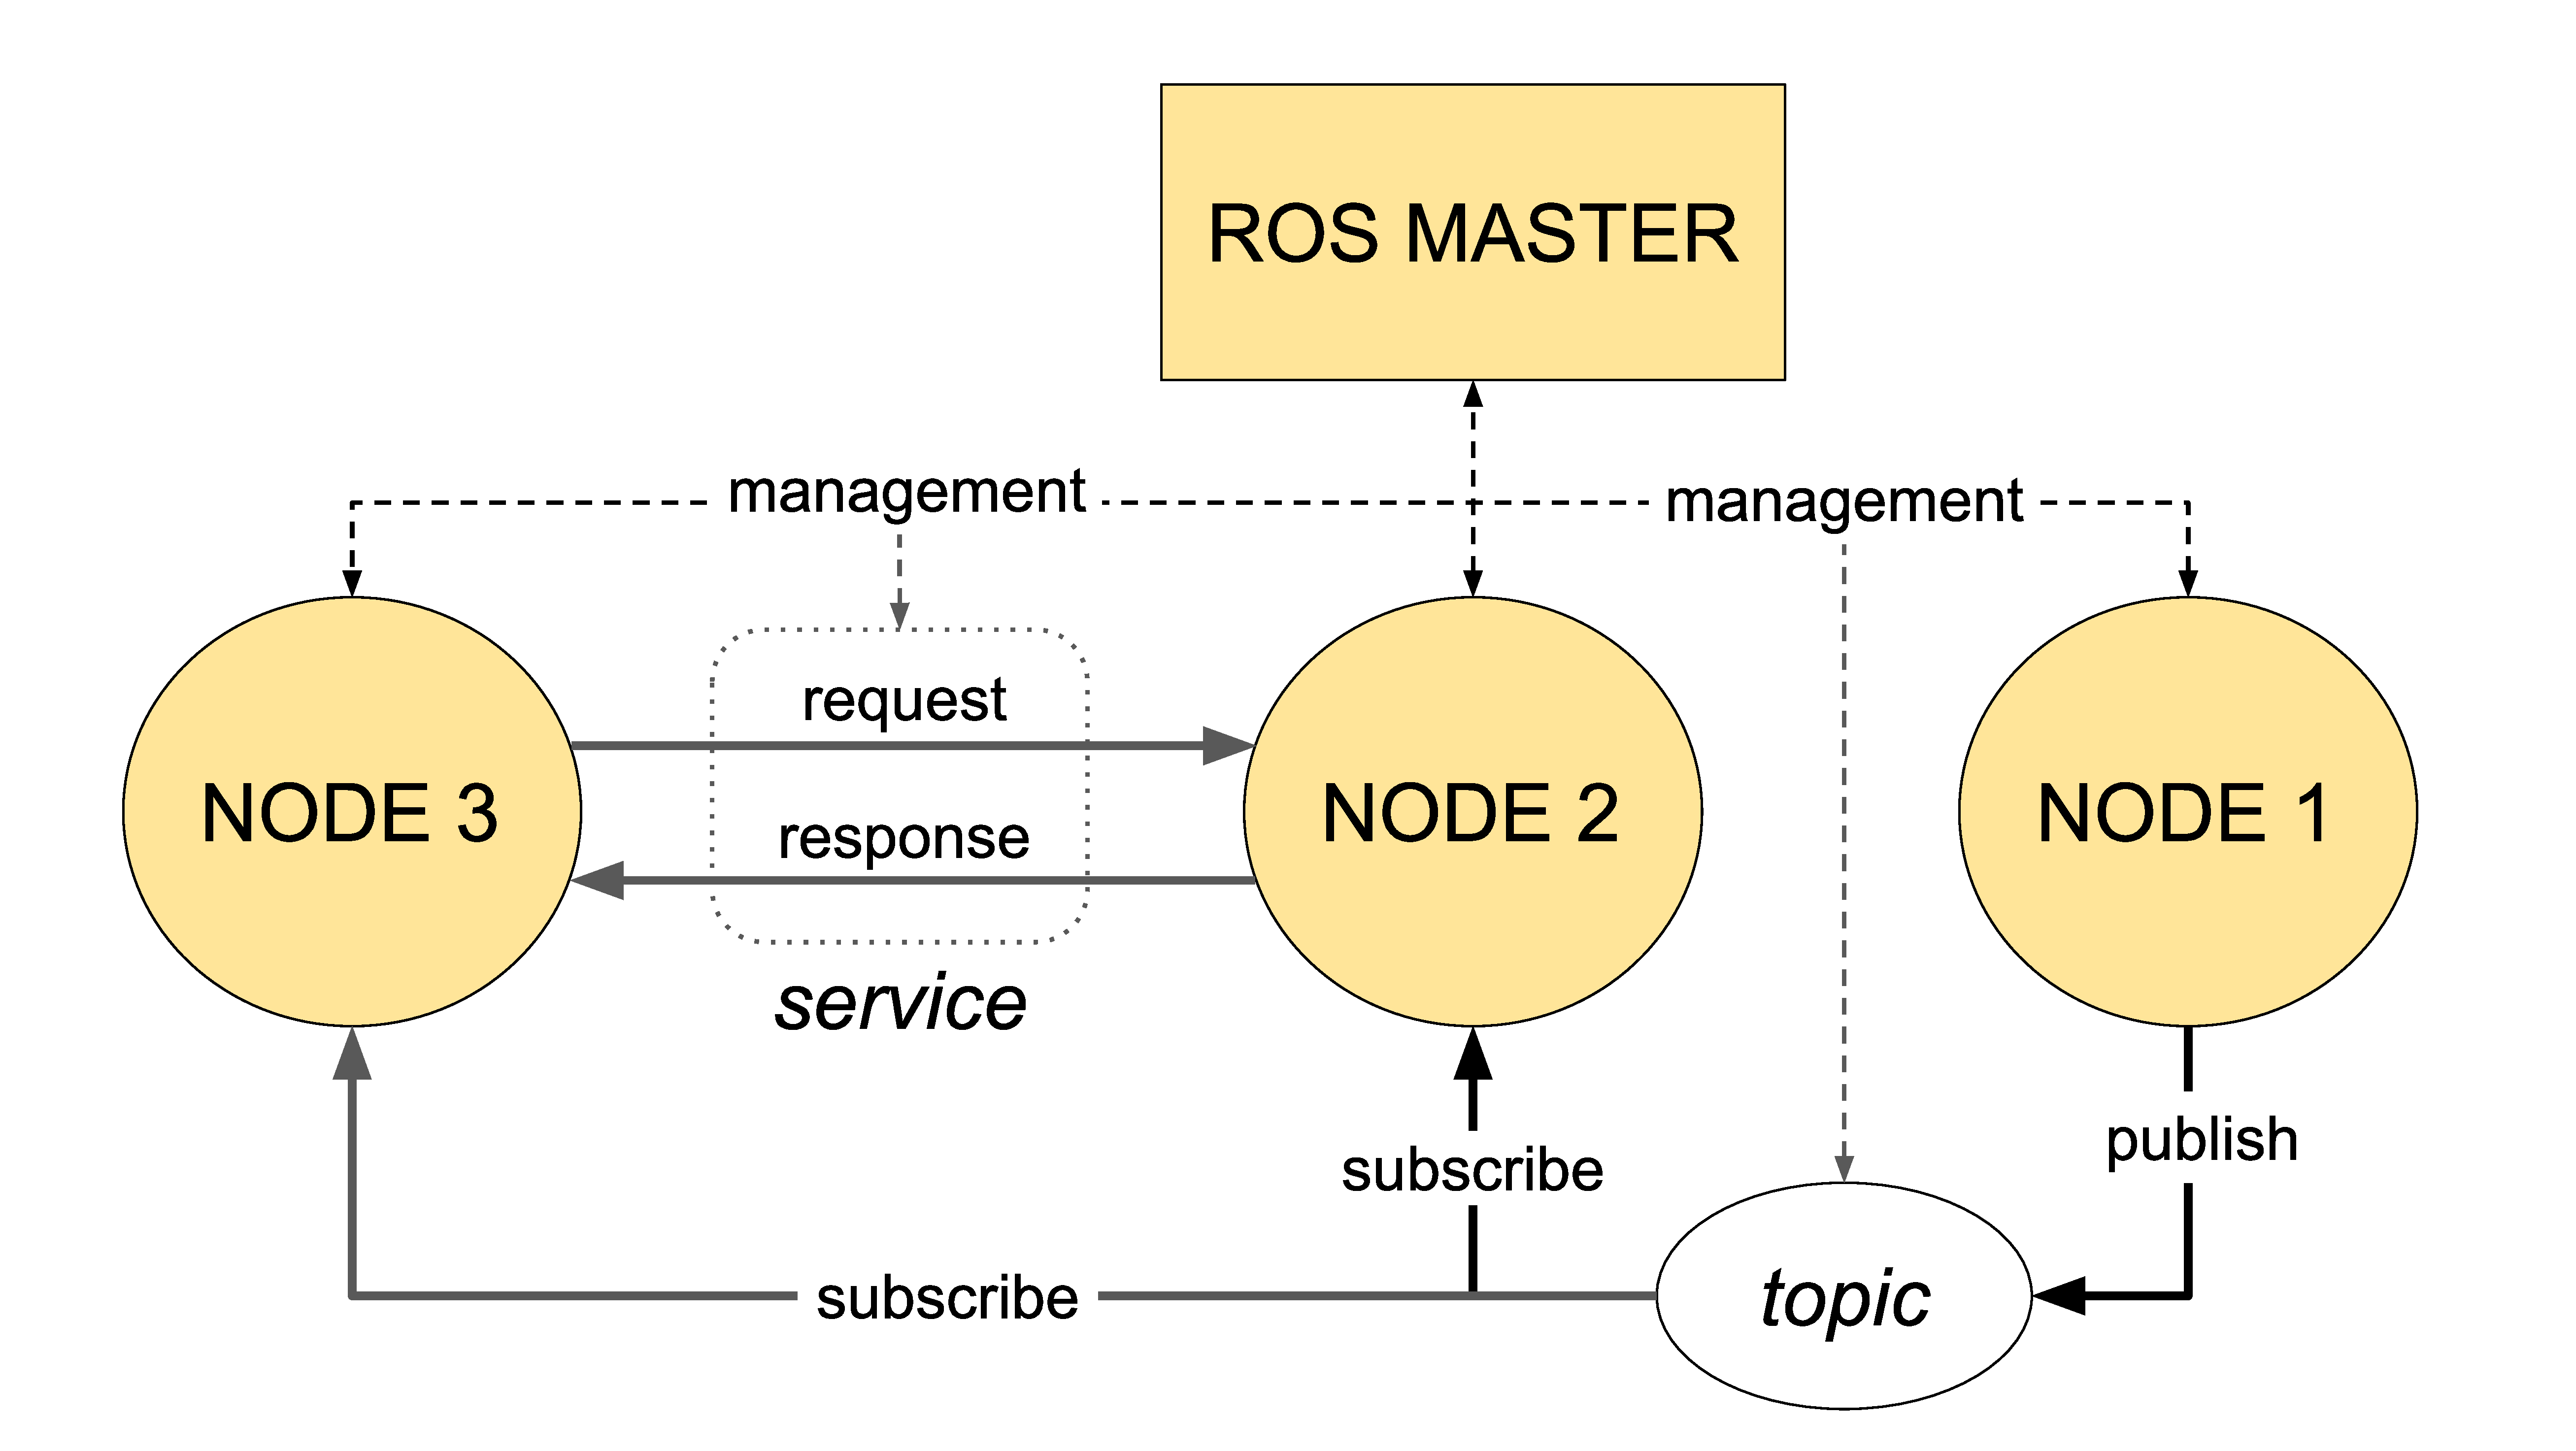
\includegraphics[width=0.8\textwidth]{./fig/photos/ros_schema.eps}
    \caption{Structure of \ac{ROS} communication model. Individual \textit{nodes} share data using \textit{topics} (publisher-subscriber model) or \text{services} (request-response model). The whole communication as well as \textit{node} registration in managed by \textit{master}.}%\url{https://www.clearpathrobotics.com/assets/guides/melodic/ros/Intro%20to%20the%20Robot%20Operating%20System.html}}
    %\label{fig:minipix}
\end{figure}

\subsection{simulations}
The simulations within this project were made using \textbf{Gazebo}, an open-source 3D simulator for robotic research.
It is fully compatible with \ac{ROS} and allows realistic simulations of robotic systems.
The ionizing radiation was simulated using \textbf{Rospix}\footnote{available at: \url{https://github.com/rospix}} simulation package.
The simulation process incorporates properties of the environment (air attenuation) as well as the geometry of the sensor and all the underlying principles leading to the detection of an ionizing photon by the Compton camera.
The properties of the simulator of ionizing radiation are described in \cite{baca2019timepix}.

\section{MRS UAV system}
The proposed high-level control method builds on the MRS UAV system\footnote{available at: \url{https://github.com/ctu-mrs/mrs_uav_system}} \cite{mrs_system}.
The MRS UAV system is a research-oriented software platform developed at Czech Technical University in Prague.
The MRS system is based on \ac{ROS} and provides full control pipeline for different types of \ac{UAV}s, including state estimation, sensor fusion, trajectory generation, multi-robot communication, planning and feedback control.
Methods proposed in this thesis builds on some parts of the MRS UAV System --- localization and state estimation (it is assumed the drones are localized using \ac{GPS} or other localization method), communication (the drones can exchange information between each other) and control (the \ac{UAV}s can execute given path).


%%%%%%%%%%%%%%%%%%%%%%%%
%%%%%%%%%%%%%%%%%%%%%%%%%%
%%%%%%%%%%%%%%%%%%%%%%%
%%%%%%%%%%%%%%%%%%%%%%%%%%%%
%%%%%%%%%%%%%%%%%%%%%%%%%%
%%%%%%%%%%%%%%%%%%%%%%%%
%%%%%%%%%%%%%%%%%%%%%%%%%%
%%%%%%%%%%%%%%%%%%%%%%%
%%%%%%%%%%%%%%%%%%%%%%%%%%%%
%%%%%%%%%%%%%%%%%%%%%%%%%%

% %%{
\mycomment{



\begin{figure}[!h]% %%{
  \centering
  \subfloat[\centering Cross-section for photon interactions in Silicon in the MeV range. The four dominating interaction mechanisms are photo effect, Compton scattering, pair creation and Rayleigh scattering. Source: \cite{zoglauer}] {
    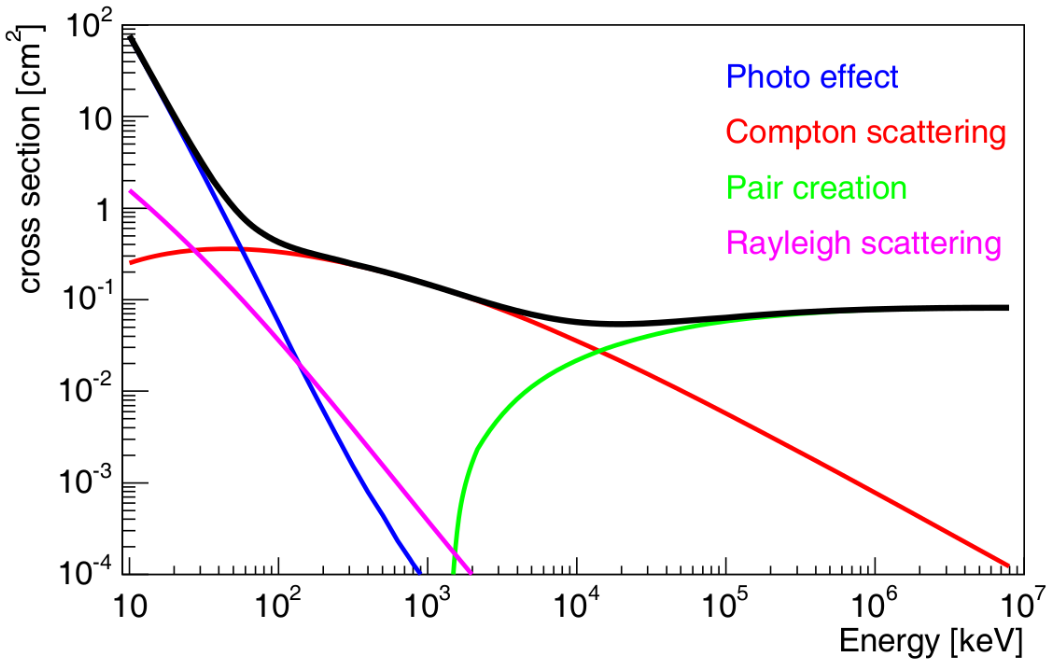
\includegraphics[width=0.2\textwidth]{./fig/photos/cross_stat.png}
    \label{fig:aaaaaa}
  }
  \subfloat[\centering Cross section for compton scattering. Source: \cite{zoglauer}] {

    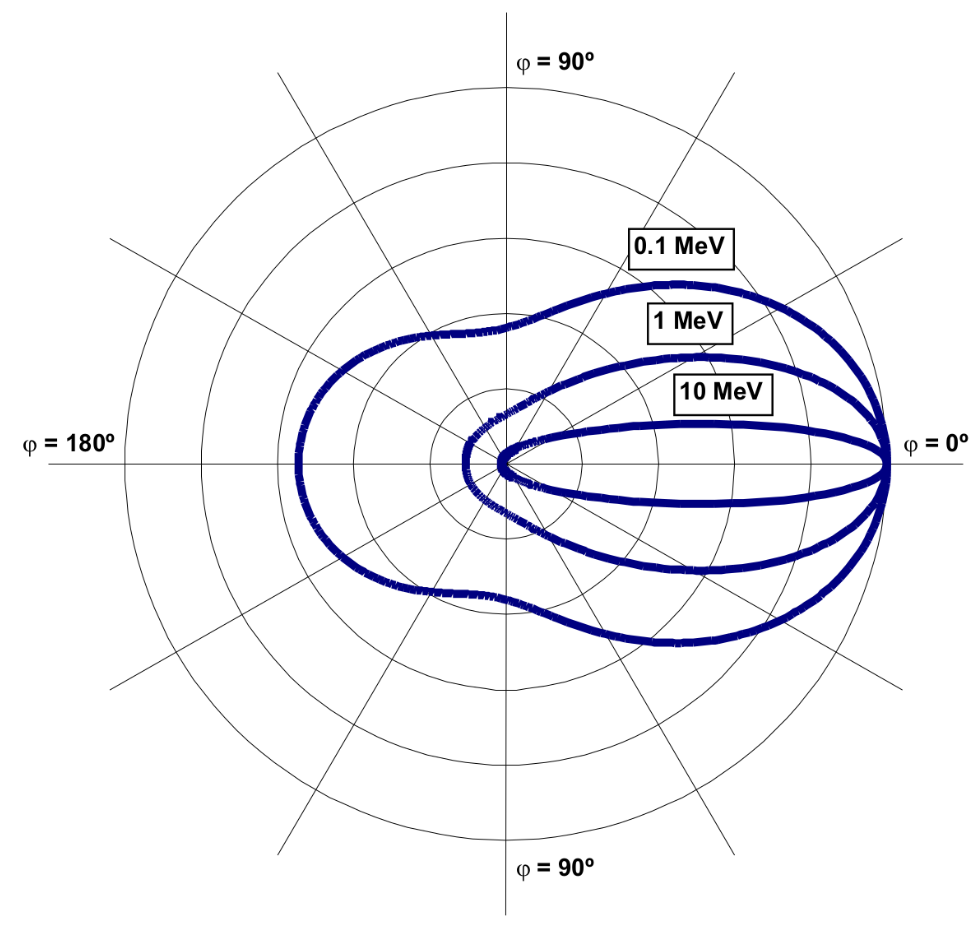
\includegraphics[width=0.2\textwidth]{./fig/photos/cross_section.png}
    \label{fig:aaaaaa}
  }
  \caption{TODO}
  \label{fig:xxx}
\end{figure}% %%}
  \section{Radioactive decay}
  Radioactive decay is a process where an unstable atomic nucleus transforms into a lower-energy state.
  During this process, it loses energy by radiation.
  There are three main types of such radiation - alpha, beta and gamma.
  Whereas alpha particles can be stopped by a sheet of paper and beta particles by aluminium shielding, gamma particles can be blocked only using a thick block of lead or a massive concrete wall.
  Moreover, highly energetic gamma rays have a negative effect on the human body, causing damage on a cellular level.
  Being exposed to such radiation poses a risk of severe health problems or death.

  \section{Some properties of $\gamma$ radiation}
  \subsection{Inverse square law}
  \subsection{Interaction with matter}

  The quantity of emitted particles ("strength" of the source) is expressed in Becquerels.
  It is a SI unit defined as the number of emitted particles per second.

  \section{Interaction with matter}
  As the gamma particle passes through matter, there are three possible effects that might happen:
  \textbf{the photoelectric effect}, \textbf{Compton scattering} and \textbf{pair production}.

  \textbf{The photoelectric effect} is typical at low energies of gamma rays. A photon undergoes an interaction with an electron that is bound in an atom. The incident photon completely disappears in this interaction. A product of this interaction is a photon.
  \textbf{The Compton effect} is typical for mid-energetic gamma rays. In this process, an incident gamma photon loses energy to an atomic electron. A new lower energetic photon is emitted in a different direction (hence the frequently used term "Compton scattering").
  \textbf{Pair production} is typical for high-energetic gamma rays. It is a process in which a photon of sufficient energy is converted into an electron and a positron.

  The Compton effect (published in 1923 \cite{}) describes the way how a (gamma or X-ray) photon interacts with a static electron. An incident photon with wavelength $\lambda$ losses some energy to the electron. A new lower energetic photon with wavelength $\lambda^{\prime}$ is emitted under angle $\beta$. Thanks to the law of conservation of energy and momentum, Compton derived the following equation
  \begin{equation}
      \lambda^{\prime} = \lambda + \frac{h}{m_{e}c}(1-\mathrm{cos} \beta),
  \end{equation}
  where $\lambda$ is the wavelength of the incident photon, $\lambda^{\prime}$ is the wavelength of the emitted photon, $h$ is the Planck constant, $m_{e}$ is the electron rest mass, $c$ is the speed of light and $\beta$ is the scattering angle.

  \begin{figure}[!h]
      \centering
      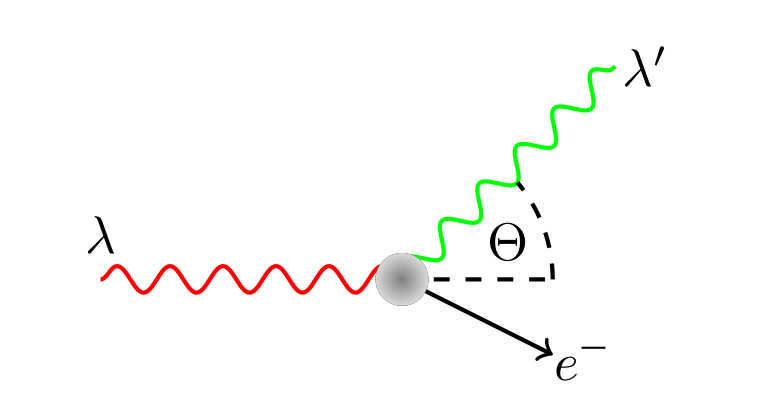
\includegraphics[width=0.3\textwidth]{./fig/photos/scattering.png}
      %\label{fig:scattering}
      %\caption{An illustration of Compton scattering. The incident photon interacts with the static electron. As a result, a new lower energetic photon is emitted in a direction changed by $\beta$ as part of its energy is transferred to electron $e^{-}$. Source: \cite{baca2021gamma}}
  \end{figure}


  \subsection{Klein Nishina formula}
  TODO

  \subsection{Compton effect}
  TODO


  \section{Compton camera}
  This effect is the fundamental principle in a sensor called a Compton camera. 
  The sensor is typically composed of two main components: the scatterer and the absorber. 
  The incident photon first interacts with the scatterer, where the lower energetic photon is emitted under angle $\beta$ (thanks to the Compton effect). 
  Since it is more common to measure energies instead of wavelength, we can rewrite the Compton formula as
  \begin{equation}
  E_{\lambda^{\prime}} = \frac{E_{\lambda}}{  1 + (E_{\lambda} / m_{e}c^{2}) (1 - \mathrm{cos} \beta)},
  \end{equation}
  where $E_{\lambda}$ is the energy of the incoming photon from the source, $E_{\lambda^{\prime}}$ is the energy of the scattered photon.  
  The bi-product of the interaction (electron $e_{e^{-}}$) is immediately measured in the scatterer, and its position is recorded.
  Then, the scattered lower energetic photon interacts with the second layer of the sensor - the absorber. 
  The photoelectric effect is witnessed while measuring the product of it - the energy of the electron $e_{\lambda^{prime}}$ and its position on the absorber.

  Now we can express the scattering angle $\beta$ as
  \begin{equation}
      \beta = \mathrm{arccos} \left (  1-\frac{m_{e}c^{2}E_{\lambda^{\prime}}}{E_{\lambda} (E_{\lambda} - E_{\lambda^{\prime}})} \right )
      %\label{eq:compton_beta_formula}
  \end{equation}

  Given the measurements on the scatterer and absorber and computed scattering angle $\beta$ using the equation \ref{eq:theta} (using known energy of the incoming photon $E_{\lambda}$), we can reconstruct a set of possible directions from where the original photon arrived. Since the Compton effect is symmetrical, the set of possible directions towards the source of ionizing radiation forms a surface of a cone.



  \subsection{MiniPIX TPX3 sensor}
  The sensor used in this work is a small CdTe event-based camera that is capable of witnessing the interactions between gamma photons and the matter of the sensor and reporting them in real time.
  Unlike the traditional model of the Compton camera mentioned before, this is a single-stack detector.
  In other words, there is no distinction between the scatterer and the absorber and all the measurable interactions are happening in one 14x14x2 mm block of CdTe semiconductor material.
  The sensor is capable of measuring a 3D position of the interactions (and distinguishing its type) inside the detector with nanosecond resolution. 
  All these features open the possibility of using it in Compton camera mode.
  Technical details of the sensor are described in \cite{baca2021gamma} and \cite{baca2019timepix}.
  The biggest advantage of this sensor is its small size, low weight and low power consumption.
  Thanks to that, we can use this sensor on board a small UAV. 


  \section{Cs137}

  \section{ROS}

  \section{MRS UAV system}
}
% %%}

%!TEX root = ../main.tex
\chapter{Methods for Compton imaging\label{chap:mlem_theory}}
The 3D reconstruction of sources of ionizing radiation poses a challenging problem.
The difficulty of this task lies in the fact that the detected $\gamma$ particle could originate anywhere on the surface of the reconstructed Compton cone.
Several methods for Compton imagining have been investigated in the past.
This chapter provides a brief overview of such methods and describes the theoretical background of the \ac{MLEM} method.

\section{Compton imagining in nuclear medicine}
The problem of reconstructing 3D positions of sources of ionizing radiation has been studied in depth in the field of medical imaging, where it is used as a non-invasive method for diagnostics.
To give an example:
In cancer diagnostics, a small amount of radioactive substance (called a tracer) is injected into the patient's vein.
The tracer is absorbed by different parts of the body in varying amounts, which can show areas with abnormal metabolic activity, which is usually the case for cancer cells.
The detection of emitted particles and 3D reconstruction of their sources allow doctors to find the location of the tumour in the patient's body.

\section{Differences}
Compton imaging in medical applications typically requires a high resolution of the reconstructed image.
The distances between source and detector are small (tens of centimetres), number of measured events is high (tens of thousands and more).
The reconstruction process is typically performed offline (all measurements are collected first, and then the algorithms process the data) since there is no need for online estimation, and the processing of measured data might take non-negligible time.
The domain of multi-robot radiation mapping has multiple differences compared to the medical field.
The distance between the source and detector is much larger (from meters to tens of meters).
The \ac{UAV}s have limited payload (hence the detector carried on board must be light and compact).
It results in the fact that the number of measurements is much lower (hundreds-thousands detected Compton events).
Moreover, we would like to reconstruct the sources of ionizing radiation in real-time.
Despite all of these differences, the aim of this work is to get inspiration in the medical field and apply these algorithms to the given problem.

\section{Reconstruction methods}
The reconstruction methods can be divided into two categories: analytical (direct) and iterative algorithms \cite{lojacono2}.
\subsection{Analytical reconstruction methods}
In analytical methods, the aim is to find a solution directly from the conical projections of reconstructed Compton events.
Such a solution might be exact in the continuous model (e.g. computing the exact intersection point of all acquired Compton measurements), yet impractical in real-world applications, where the measurements might be noisy (thus, conical surface projections might not intersect the real position of the source) or where the computational power is limited.
To illustrate the difficulties of direct reconstruction methods, the algorithm proposed in \cite{baca2021gamma} estimates the initial hypothesis of the source position as a point that is closest to all measured cone surfaces (which might be considered an analytical method).
Finding a solution to the nonlinear least squares problem is computationally demanding and tractable only for a small number of cones.
Another example of a simple direct reconstruction method is called back-projection.
\subsubsection{Back-projection}
Back-projection is one of the simplest reconstruction methods. 
The Compton cones are projected to the (discretized) space of possible source locations, and each bin records the number of cones intersecting its position. 
The bins with more intersections are considered as possible source positions.
The back-projection for 2D image reconstruction is illustrated in figure \ref{fig:bppp}.
The advantage of back-projection method is its simplicity and the fact that it can be easily parametrized when processing a large number of measurements.
On the other hand, the back-projection requires a significant number of data in order to make the reconstruction accurate and does not take into account the properties of the detector.
  \begin{figure}[!h]
    \centering
      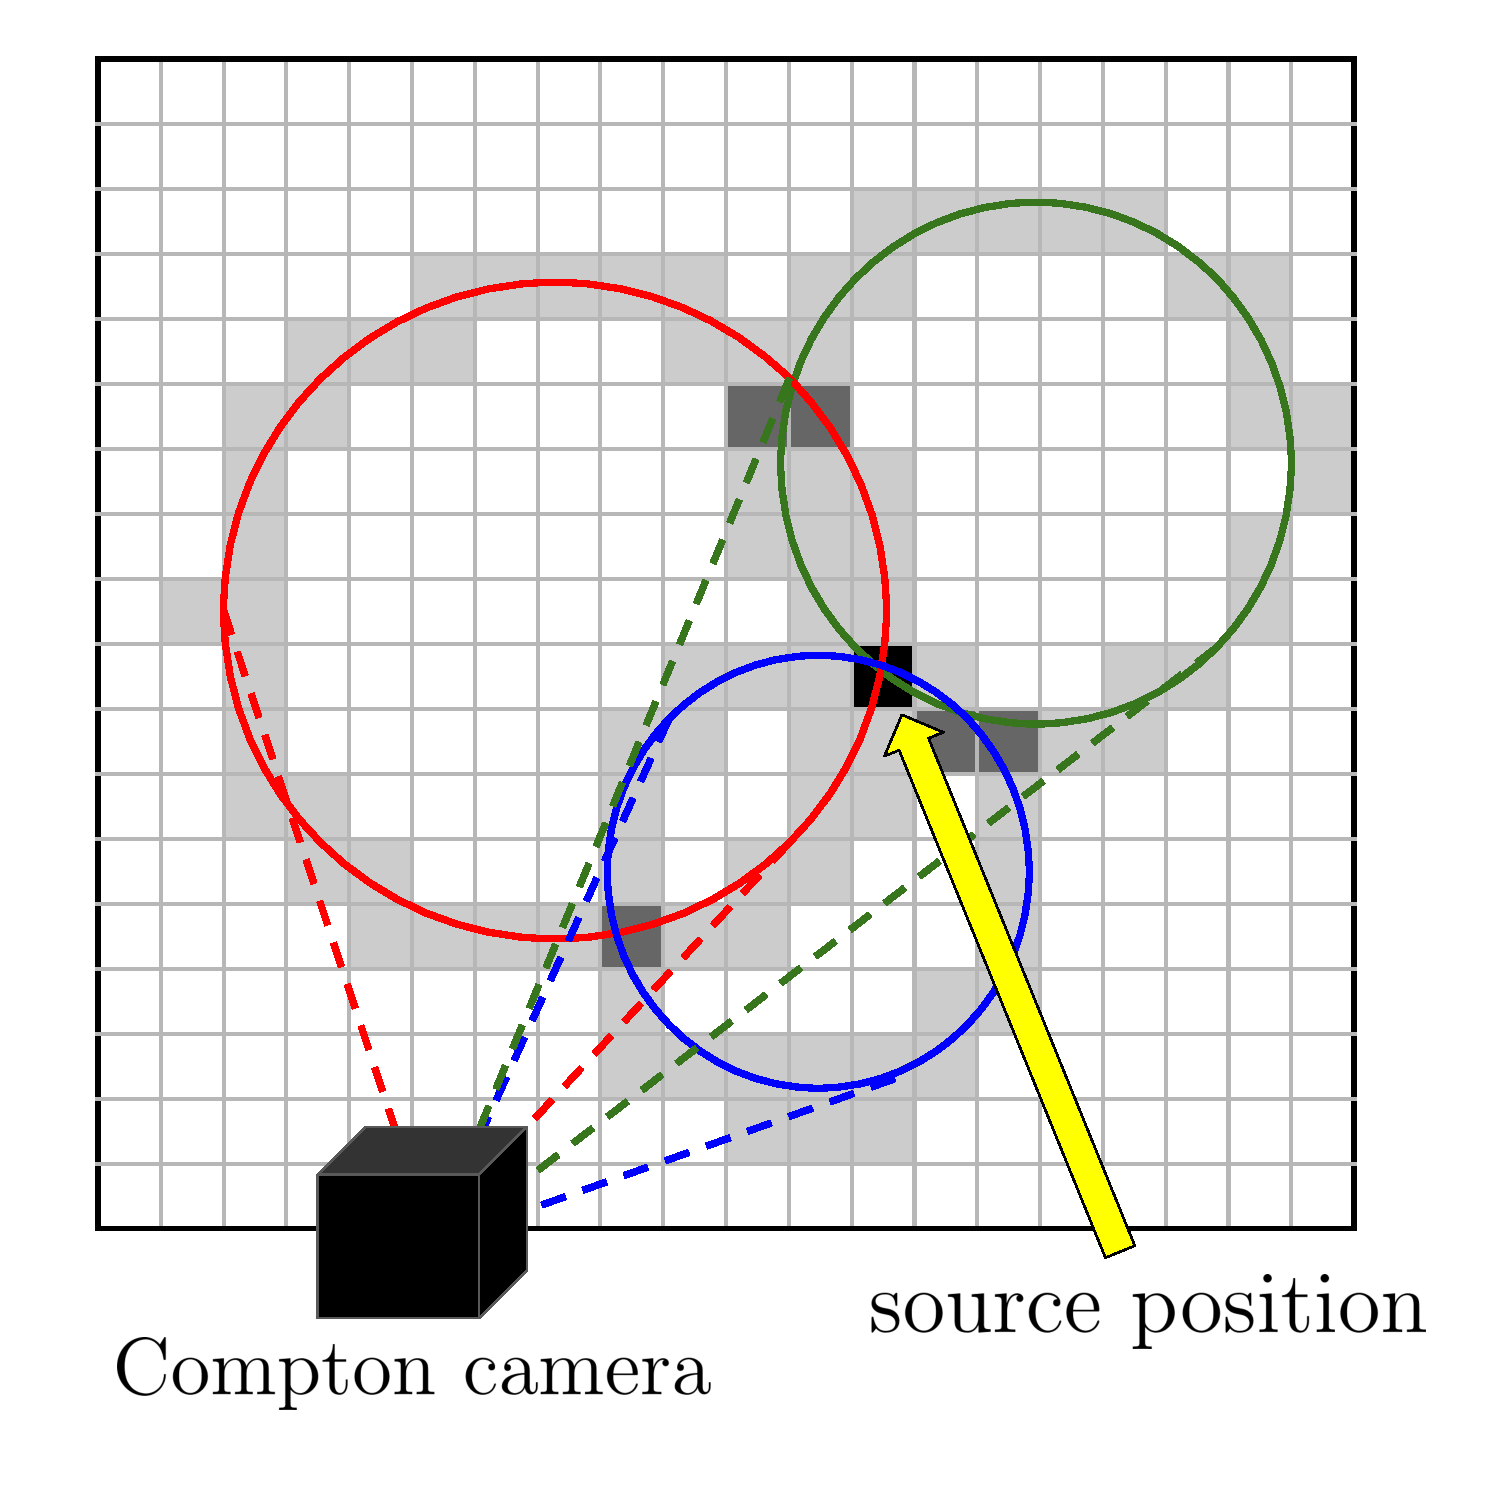
\includegraphics[width=0.5\textwidth]{./fig/photos/back_proppp.eps}
    \caption{Simple back-projection reconstruction method illustrated in 2D. Recorded Compton cones are back-projected to the space of possible source positions. The number of cones intersecting each bin is computed, as illustrated by the white-grey-black cell colours.}
    \label{fig:bppp}
  \end{figure}

\subsection{Iterative reconstruction methods}
The iterative reconstruction methods approximate the positions of sources by iteratively adapting the reconstruction to the measured projections.
Each iteration improves the current estimate based on the recorded measurements (the Compton cones), starting from some initial estimate or prior belief of sources distribution. 
The iterative approach does not provide an exact and unique solution. On the other hand, it is more flexible, can handle noise in the measurements (if it is properly modelled) and is widely used in practice.
The literature describes three main iterative reconstruction methods: \acf{MLEM}, \acf{MAP} and \acf{SOE}.
\ac{MLEM} \cite{MLEM_Shepp_1982}, \cite{MLEM_Lange_Carlson_1984}, \cite{MLEM_Wilderman_2000} is an iterative algorithm that is based on the maximum likelihood approach.
Another approach called \ac{MAP} \cite{MLEM_Lange_Carlson_1984} is based on the Bayesian approach.
It is an extension of \ac{MLEM} that allows to the incorporation of some prior knowledge about the source distribution or features of the data.
\ac{SOE} is a stochastic algorithm that randomly assigns the origins of the measured events to the conical surfaces.
During the course of reconstruction, the origins of events are stochastically moved, and the acceptance of the new event origin is determined by the change in event density.
After several iterations, the reconstructed distribution of origins converges to a quasistationary state \cite{SOE_Andreyev_2009}.

The iterative methods were originally developed for \ac{PET} and \ac{SPECT} imagining.
The \ac{PET}  method is based on positron emission. 
The emitted positron interacts with electrons in the patient's body, and both particles annihilate. 
The annihilation produces energy that comes in the form of two gamma photons that go in opposite directions.
Detection of these two gamma photons (measured by the detector at the same time) allows us to reconstruct a 3D image of the patient's body.
In \ac{SPECT}, only a single gamma ray is produced. 
Medical \ac{SPECT} imagining devices typically acquire measurements from different positions and use collimators to restrict the set of possible directions of incoming gamma radiation.
Measured events in \ac{PET} and \ac{SPECT} are stored in memory in discrete bins (each bin represents the count of reconstructed particles in a defined time interval or a subset of the image space).
The Compton camera events are represented in memory using the list-mode approach.
List-mode approach stores measured Compton cones in a list data structure, where each record contains information about the exact arrival time, position and energy of measured interactions.
Despite all these differences in the nature of the measurements, the iterative methods were also adapted for Compton imaging.

%Collimators restricts the set of possible directions from which the gamma ray may enter the detector (and be detected), therefore they can improve accuracy of the detection.
%Since only one gamma-ray is emmited (unlike in \ac{PET}), high number of measurements is needed for accute reconstruction.
%Medical \ac{SPECT} imagining cameras typically use collimators to get some information about direction of incoming gamma ray.
%Collimators restricts the set of possible directions from which the gamma ray may enter the detector (and be detected), therefore they can improve accuracy of the detection.

\section{Maximum likelihood expectation maximization}
The iterative \ac{MLEM} algorithm is widely used for image reconstruction from the Compton camera data. % \cite{maxim2016}.
The algorithm was originally proposed by \cite{MLEM_Shepp_1982} and later adapted to the Compton camera measurements and list-mode form by \cite{wilderman}.
As the name suggests, the algorithm is based on maximizing the likelihood of measured data.

\subsection{Maximum likelihood estimation}
\ac{MLE} is a classical approach in machine learning.
\ac{MLE} method is used to estimate the parameters of a probability distribution based on observed data. 
The goal of \ac{MLE} is to find the parameter values that make the observed data most probable under the assumed probability distribution.
This is done by calculating the likelihood function, which is the probability of the observed data given a set of parameter values.
The likelihood is defined as 
\begin{equation}
  \mathcal{L}(\boldsymbol{O}| \Phi) = p(\ \mathrm{observing\ measurements} \  \boldsymbol{O} \ \mathrm{given\ parameters\ } \Phi ).
  \label{eq:likelihood}
\end{equation}
We want to maximize this expression with respect to the hidden parameters.
In other words, we want to find such parameters that fit our observations in the best possible way.

\subsection{Original MLEM formulation}
Let us divide the area of possible sources of radiation into $J$ discrete bins (each indexed with $j$, where $j = 1 \dotsc J$).
%Each discrete bin is often represented by its centre position.
Suppose the binned data space of all measured events is $\mathbf{I}$, divided in $I$ discrete bins indexed with $i$, $i = 1 \dotsc I$.
The unobservable data space of all not measured events is denoted $\mathbf{\hat{I}}$.
Let us define the vector of measurements $\mathbf{Y}$ with elements $y_{i}$ ($i \in \{1, \dots I\}$)representing the number of particles detected in the corresponding bin $i$.
Let us define matrix $\mathbf{T}$ ($\mathbf{T} \in \mathbb{R}^{I \times J}$), where each position in the matrix is defined as
\begin{equation}
  t_{ij} =  P(\textrm{detected in } i | \textrm{emitted from } j).
\end{equation}
In other words, $t_{ij}$ represents the probability that we observe observation $i$ given that a radioactive particle that caused the observation $i$ has been emitted from position $j$.
Let us assume that the number of photons emitted from one position $j$ is a discrete random variable that follows a Poisson distribution with the expected value $\lambda_{j}$.
Our goal is to estimate vector $\bm{\lambda}$ with elements $\lambda_{j}$ ($j \in \{1 , \dots, J\}$), each corresponding to the expected intensity of emission from the position $j$.

%(the algorithm was originally developed for \ac{PET} imaging, where $y_{i}$ can be arbitrary number, $y_{i} = 1$ in list-mode representation).
Let us assume (for the purpose of the algorithm's derivation) that the matrix $\mathbf{T}$ is known.
Then a vector $\bm{\mu}$ can be defined, where each element of $\bm{\mu}$ 
\begin{equation}
  \mu_{i} = \sum_{j} t_{ij}\lambda_{j}
  \label{eq:mu}
\end{equation}
denotes the average number of events measured in bin $i$.
The probability of measuring $y_{i}$ particles in the measurement bin $i$ with respect to some given average emission intensity $\bm{\lambda}$ is then expressed as (Poisson distribution):
\begin{equation}
  p(y_{i} |\mu_{i} ) = e^{-\mu_{i}} \frac{\mu_{i}^{y_i}}{y_{i}!}.
\end{equation}
The likelihood of all the measurements (assuming the events to be independent) is
\begin{equation}  
  \mathcal{L}(\mathbf{Y} | \mathbf{\lambda}) = \prod_{i}p(y_{i} |\mu_{i} ) = \prod_{i} e^{-\mu_{i}} \frac{\mu_{i}^{y_i}}{y_{i}!}.
  \label{eq:prod}
\end{equation}
We want to maximize the likelihood by finding the best possible values of $\bm{\lambda}$. 
The maximum likelihood solution is:
\begin{equation}
  \mathbf{\lambda}_{best} = \underset{\mathbf{\lambda}}{\mathrm{argmax}}( \mathrm{log}\ \mathcal{L}(\mathbf{Y} | \mathbf{\lambda})).
\end{equation}
Instead of maximizing the product in equation \ref{eq:prod}, it is common to maximize its logarithm since the logarithm is a monotonically increasing function.
After taking the logarithm of \ref{eq:prod} and substitution $\mu_{i} = \sum_{j} t_{ij}\lambda_{j}$, we have the following:
\begin{equation}  
  \mathrm{log}\ \mathcal{L}(\mathbf{Y} | \mathbf{\lambda}) = \sum_{i}\left ( -\sum_{j} t_{ij}\lambda_{j} + y_{i} \mathrm{log}(\sum_{j} t_{ij}\lambda_{j})  - \mathrm{log}(y_{i}!) \right ).
  \label{eq:likelihood1}
\end{equation}
However, the nonlinear equation \ref{eq:likelihood1} can not be maximized directly.
The solution is to use an iterative \ac{EM} algorithm, as proposed in \cite{MLEM_Lange_Carlson_1984}.
\subsection{Expectation maximization algorithm}
The \ac{EM} algorithm was originally described in \cite{EM}. 
It is an iterative algorithm consisting of two steps performed in each iteration --- E-step and M-step.
The iterations of ac	
The vector of hidden parameters  $\mathbf{\hat{\lambda}}^{[l = 0]}$ we would like to find is initialized to some starting value using back-projection of the Compton cones or with uniform distribution.
The purpose of the E-step is to determine the expectation of the likelihood function given the measurements $\mathbf{Y}$ and the estimation of hidden parameters $\mathbf{\hat{\lambda}}^{[l-1]}$ obtained from the previous iteration. 
Then in the M-step, this expectation is maximized by setting its derivatives (with respect to $\mathbf{\hat{\lambda}}^{[l-1]}$) to $0$.
According to \cite{MLEM_Lange_Carlson_1984}, the final formula for iterative \ac{MLEM} algorithm with binned data is 
\begin{equation}
  \hat{\lambda}_{j}^{[l]} = \frac{\hat{\lambda}_{j}^{[l-1]}}{\sum_{i}t_{ij}} \sum_{i \in I} \frac{t_{ij} y_{i}}{\sum_{k} t_{ik} \hat{\lambda}_{k}^{[l-1]}}.
  \label{eq:mlem_class}
\end{equation}
The term $\sum_{i}t_{ij}$ is called sensitivity of detection $s_{j}$ and presents the probability that particle emitted at position $j$ is detected by the sensor:
\begin{equation}
  s_{j} = P(\textrm{detected by the sensor}\ | \textrm{emitted from } j) =  \sum_{i}t_{ij}.
\end{equation}
\subsection{List-mode Maximum Likelihood Expectation Maximization}
The list-mode extension of \ac{MLEM} for the Compton imaging was proposed in \cite{wilderman}.
Each measurement bin $i$ in list-mode \ac{MLEM} consists of only one detected Compton event.
Therefore the number of detected events $y_{i}$ in data bin $i$ is either $y_{i} = 1$ for the detected event or $y_{1} = 0$ when no event was recorded.
This simplifies the formula \ref{eq:mlem_class} to
\begin{equation}
  \hat{\lambda}_{j}^{[l]} = \frac{\hat{\lambda}_{j}^{[l-1]}}{s_{j}} \sum_{i \in \mathbf{I}}\frac{t_{ij} }{\sum_{k} t_{ik} \hat{\lambda}_{k}^{[l-1]}}.
  \label{eq:lmmlem}
\end{equation}
We denote as \ac{MLEM} the list-mode \ac{MLEM} algorithm for Compton imaging formulated in \ref{eq:lmmlem} in the rest of the thesis for simplicity.
Since only recorded measurements are considered in the list-mode approach, it no longer holds that sensitivity of measurements can be expressed as $s_{j} = \sum_{i}t_{ij}$ (summation over all measurement bins $i$).
The sensitivity of detection is then a sum over all events \{$\mathbf{I} \cup \mathbf{\hat{I}}\}$, not only those that were measured, therefore $s_{j} = \sum_{\mathbf{I} \cup \mathbf{\hat{I}}} t_{ij}$ for Compton imaging.
%The computational complexity of the \ac{MLEM} algorithm is $\mathcal{O}(I J)$
\subsection{MLEM algorithm in practical application}
The equation \ref{eq:lmmlem} presents the formulation of the iterative \ac{MLEM} algorithm maximizing the likelihood of measured data.
The system matrix $\mathbf{T}$ and vector of sensitivity values $\mathbf{S} \in \mathbb{R}^{J}$ with elements $s_{j}$ depend on the particular geometry of the used sensor and need to be derived individually in each application.
The proposed definition of system matrix $\mathbf{T}$ and sensitivity vector $\mathbf{S}$ is described in the following chapter. 

Several other design choices are to be made in practical applications, such as setting the number of iterations of the \ac{MLEM} algorithm.
The number of iterations in \ac{MLEM} represents a balance between contrast recovery (quality of reconstruction) and image noise amplification, as stated in \cite{handheld_mlem_reconstruction}.
There is no general rule on how to set the optimal number of iterations --- it depends on the particular application, level of noise etc.
Therefore the number of iterations is set arbitrarily within this project based on the experiments with recorded real-world data.






%%%%%%%%%%%%%%%%%%%%%





%Another design-choice is the initialization of the vector $\mathbf{\hat{\lambda}}^[l = 0]$.



%Since the data for \ac{CC} are stored using list-mode approach, the $y_{i}$ (number of detected events in data bin $i$) in equation \ref{eq:mlem_class} is either $0$ or $1$.



%\section{Imagining in nuclear medicine}
%The problem of reconstructing 3D positions of sources of ionizing radiation has been studied in depth in the field of medical imagining.
%To give an example: one possible application of such methods is a cancer diagnostics.

%There are numerous methods used in medical imagining. 
%Two main approaches are following: \ac{PET} and \ac{SPECT}.
%\ac{PET} imagining typically use a gamma emitting radioisotope as a tracer.  
%The method is based on positron emission. 
%The emitted positron interacts with electron in the patients body and both particles vanish in a burst of energy. 
%This energy comes in a form of two gamma rays, that goes into a opposite directions.
%Detection of these two gamma rays (measured by the camera at the same time) allows us to reconstruct 3D image of the patient's body.
%In \ac{SPECT}, single gamma ray is produced. 
%The reconstructed image is computed from gamma rays detected by the camera.
%Since only one gamma-ray is emmited (unlike in \ac{PET}), high number of measurements is needed for accute reconstruction.
%Medical \ac{SPECT} imagining cameras typically use collimators to get some information about direction of incoming gamma ray.
%Collimators restricts the set of possible directions from which the gamma ray may enter the detector (and be detected), therefore they can improve accuracy of the detection.

%Another type of sensor (that can be used in \ac{SPECT} imagining) is a Compton camera.
%The biggest benefit of compton camera is that it provides information about the direction of detected incoming gamma ray without the use of collimator.
%The nuclear medicine reconstruction method for compton camera measurements that served as inspiration for for this thesis is called \ac{LM-MLEM}.

%!TEX root = ../main.tex
\chapter{Compton imaging for a group of UAVs\label{chap:methods_estimation}}
The \ac{MLEM} algorithm for Compton imaging described in the previous chapter has been chosen as a suitable method for data fusion of Compton measurements acquired by a group of \ac{UAV}s.
The motivation for the use of \ac{MLEM} method is described in section \ref{sec:prelim}.
Section \ref{sec:setup} presents the adaptation of \ac{MLEM} to the task of online estimation performed by a group of \ac{UAV}s.
The definition of sensitivity and system matrix is described in sections \ref{sec:sensitivity} and \ref{sec:system}.

\section{The algorithm of choice}
\label{sec:prelim}
The algorithms for Compton imaging in nuclear medicine (described in the previous chapter) served as inspiration for the imaging method proposed in this thesis.
The algorithm of choice is \acf{MLEM} (more precisely its list-mode variant for Compton imaging) for following reasons.

Firstly, the maximum likelihood approach allows us to model factors influencing the measurements (such as air attenuation, distance between the source and the sensor of ionizing radiation,  properties of the sensor and random processes leading to the detection)
as well as cope with the stochastic nature of radioactive emission and model both in the probabilistic way.
It is also relatively easy to apply and time-proven method in the field of nuclear medicine, which has been applied in robotic sensing of ionizing radiation.

Secondly, the \ac{MLEM} can take into account not only ``positive'' measurements (the Compton events recorded by the sensor), but also ``negative'' measurements (in meaning of what was NOT measured by the sensor at given position in space).
Although the radioactive emission as well as Compton event detection are stochastic processes, the fact that an \ac{UAV} flew over some position multiple times and did not measure any Compton event is a valuable information, that might help improving the estimate.
The sensitivity of detection (that is computed during the steps of \ac{MLEM} algorithm) might serve as a map of coverage of the monitored area.
In other words, the sensitivity of detection provides information about how well was which part of the area explored by the drones equipped with the Compton cameras.

Lastly, the algorithm can be easily applied in scenario with multiple \ac{UAV}s equipped with Compton cameras.
The \ac{MLEM} method is also computationally tractable under some assumptions 
(such as relatively low number of detected events (which holds for the given scenario and type of sensor) or restriction on the set of possible sources locations)
and can be evaluated online.
The almost real time estimation is important for active search strategy, where the \ac{UAV}s may adapt to the current situation and optimize the search strategy.

\section{Online MLEM Compton imaging for group of \ac{UAV}s}
\label{sec:setup}
\subsection{Discretization and hidden parameters}
As described in the chapter \ref{chap:mlem_theory}, the \ac{MLEM} algorithm belongs to the class of iterative algorithms that work with discretized space of possible source locations.
We assume that the source of ionizing radiation is static and located somewhere on the ground.
We further assume that the \ac{UAV}s are exploring a flat outdoor area without obstacles, therefore all the potential sources of ionizing radiation are located somewhere on the flat 2D ground plane.

The area of interest (where possible sources of ionizing radiation might be located) is divided into $J$ discrete bins with resolution $r$, each of them is approximated by its center position and indexed with $j$, $j \in \{1, \dots , J\}$.
The set of all collected measurements (the Compton cones) is denoted $\mathbf{I}$.
The Compton cones are indexed with $i$, $i \in \{1, \dots, I\}$, where $I$ is the total number of cones recorded.
The vector of hidden parameters $\bm{\lambda}\in \mathbb{R}^{J}$ is defined analogously as in the previous chapter, where each element $\lambda_{j}$ represents the expected value of the Poisson distribution, specifying the expected emission rate at position $j$.
The discretization process is illustrated in figure \ref{fig:discretization}.

%multifigure discretization%%{
\begin{figure}[!h]
  \centering

  \subfloat[area of interest] {
    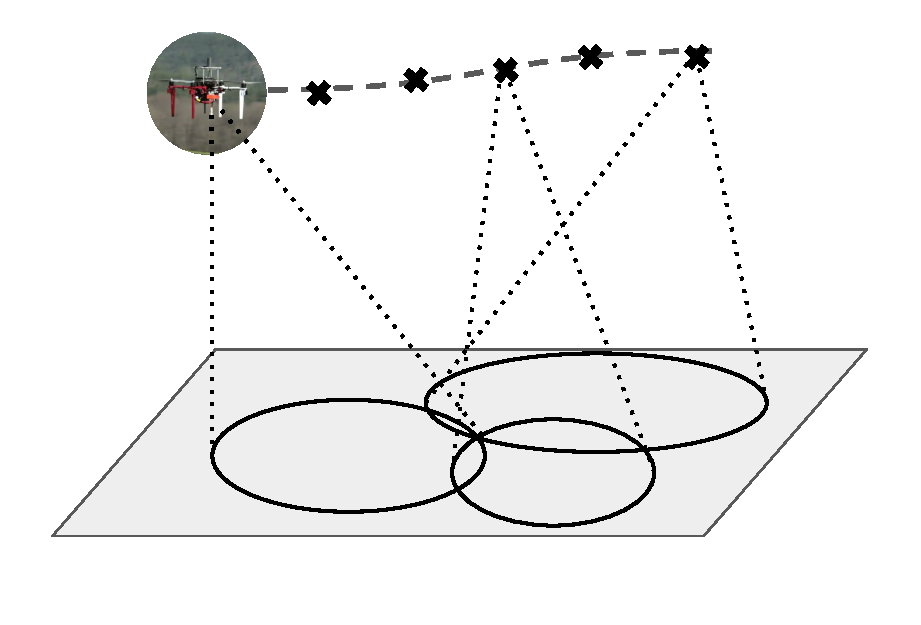
\includegraphics[width=0.32\textwidth]{./fig/photos/dis1.eps}
    \label{fig:dis1}
  }
  \subfloat[area discretized with resolution $r$] {
    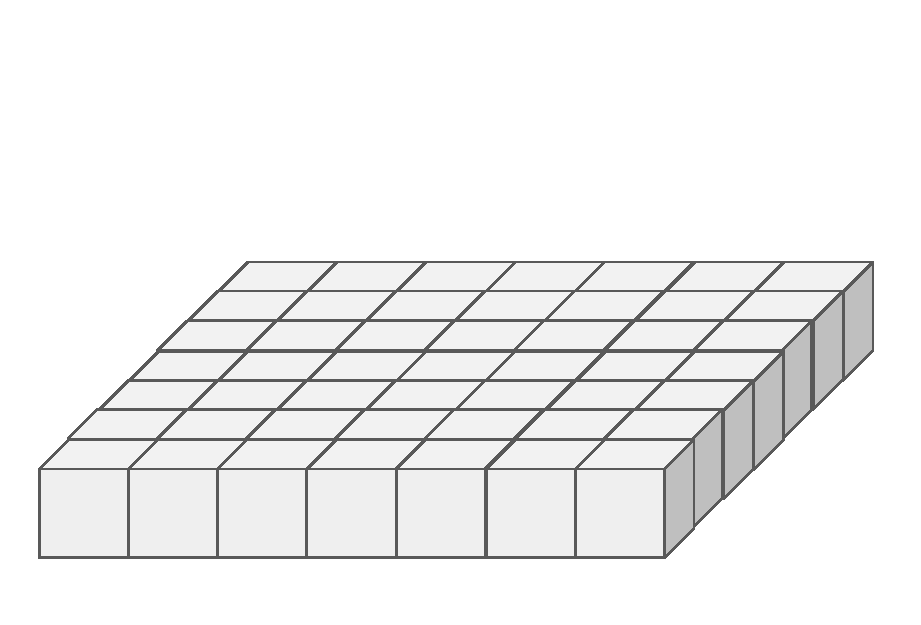
\includegraphics[width=0.32\textwidth]{./fig/photos/dis2.eps}
    \label{fig:dis2}
  }
  \subfloat[hidden parameters $\bm{\lambda}$] {
    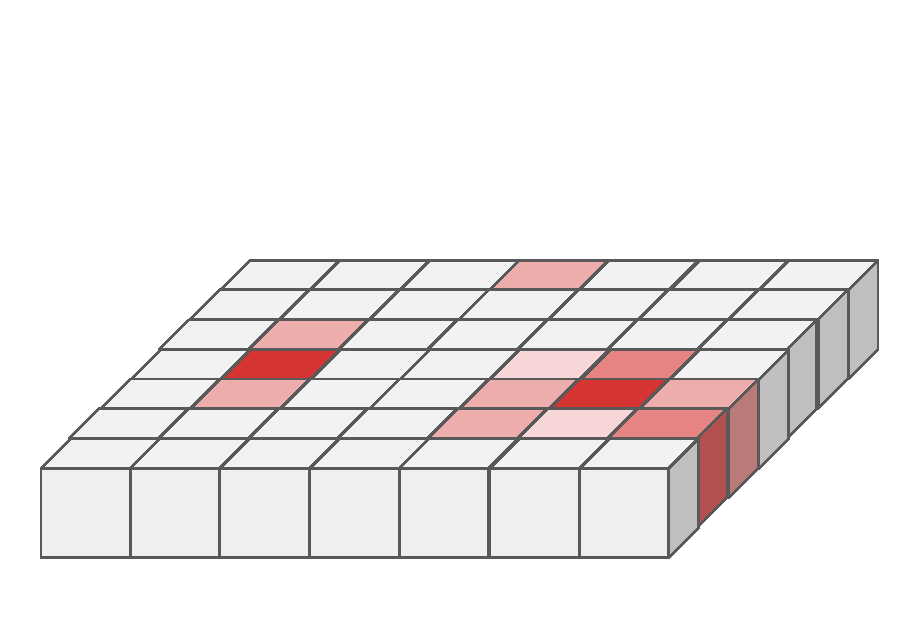
\includegraphics[width=0.32\textwidth]{./fig/photos/dis3.eps}
    \label{fig:dis3}
  }
  \caption{An illustration of the discretization of the space of possible source positions. The open area without obstacles (\ref{fig:dis1}) is discretized into $J$ discrete bins (\ref{fig:dis2}), each represented by its center position and associated with hidden parameter $\lambda_{j}$ (\ref{fig:dis3}).}
  \label{fig:discretization}
\end{figure}% %%}

\subsection{Online maximum likelihood estimation}% %%{
The estimation process proceeds interatively using the list-mode \ac{MLEM} algorithm:
\begin{equation}
  \lambda_{j}^{[l]} = \frac{\lambda_{j}^{[l-1]}}{s_{j}} \sum_{i \in I} \frac{t_{ij}}{\sum_{k} t_{ik} \lambda_{k}^{[l-1]}},
  \label{eq:MLEM}
\end{equation}
where $l$ is the current iteration of the algorithm, $\lambda_{j}$ is the hidden parameter for each position $j$ we would like to estimate, $t_{ij}$ is the element of system matrix $\mathbf{T}\in \mathbb{R}^{I \times J}$ and $s_{j}$ is the sensitivity of detection for the map position $j$.

As stated before, the \ac{MLEM} algorithm is typically used as an offline method that proceeds all the measurements at once after the end of the experiment.
Medical applications with highly sensitive detectors together with short distance between the source and the detector produce large number of measurements (tens of thousands and more) and the algorithm typically reconstructs the 3D space with high resolution.
The high number of Compton events results in the fact that the $\mathbf{T}\in \mathbb{R}^{I \times J}$ cannot be stored in the memory during the run of the algorithm and its individual elements $t_{ij}$ are recomputed in every step of the algorithm, which significantly prolongs the computing time.
If the instance of the problem (size of the sampled space $J$ and number of measurements $I$) is reasonably small, the system matrix $\mathbf{T}$ can be computed only once for each measurement and stored in the memory for future computations, which speeds up the run of the algorithm.
Furthermore, the iterations of the \ac{MLEM} algorithm can reformulated as matrix multiplication can be parallelized using \ac{GPU}.

The figure \ref{fig:online_mlem} depicts the workflow of \ac{MLEM} estimation during the experiment.
Each drone samples its current position with predefined frequency ($\SI{5}{\hertz}$).
Based on the newly sampled positions, the sensitivity of detection vector $\mathbf{s}\in \mathbb{R}^{J}$ is updated online during the experiment.
Once a new cone is detected, a new vector $\mathbf{t}_{i_{new}} = [t_{i0}, \dots,t_{ij}, \dots, t_{iJ}]$ is appended to the system matrix.
The iterative \ac{MLEM} algorithm is then repeatedly computed based o currently available sensitivity vector $\mathbf{s}$ and system matrix $\mathbf{T}$.
%Experiments showed that proposed approach is computationally tractable for scenarios with area of size $300 \times 300\ \si{\meter}$ and number 


The sensitivity vector $\mathbf{s}$ can be iteratively updated during the experiment and with constant memory requirements, since the individual elements $s_{j}$ can be update in place.

The sensitivity vector $S$ is iteratively updated using recorded drone positions, that are sampled from drone trajectories (with frequency $\SI{5}\hertz$).
The details of sensitivity computation is provided in section \ref{sec:sensitivity}.
The system matrix $\mathbf{T}$ is updated (a new row is added) every time a new Compton cone is detected.
The estimation of system matrix $\mathbf{T}$ is described in section \ref{sec:system}.

The iterative \ac{LM-MLEM} algorithm described in equation \ref{eq:MLEM} is processed regularly.
The vector of hidden parameters $\mathbf{\Lambda}$ is initialized with cones back-projection.
The \ac{LM-MLEM} estimate is recomputed every $2$ seconds.



% %%}


%figure melm online%%{
\begin{figure}[htb]
  \centering
    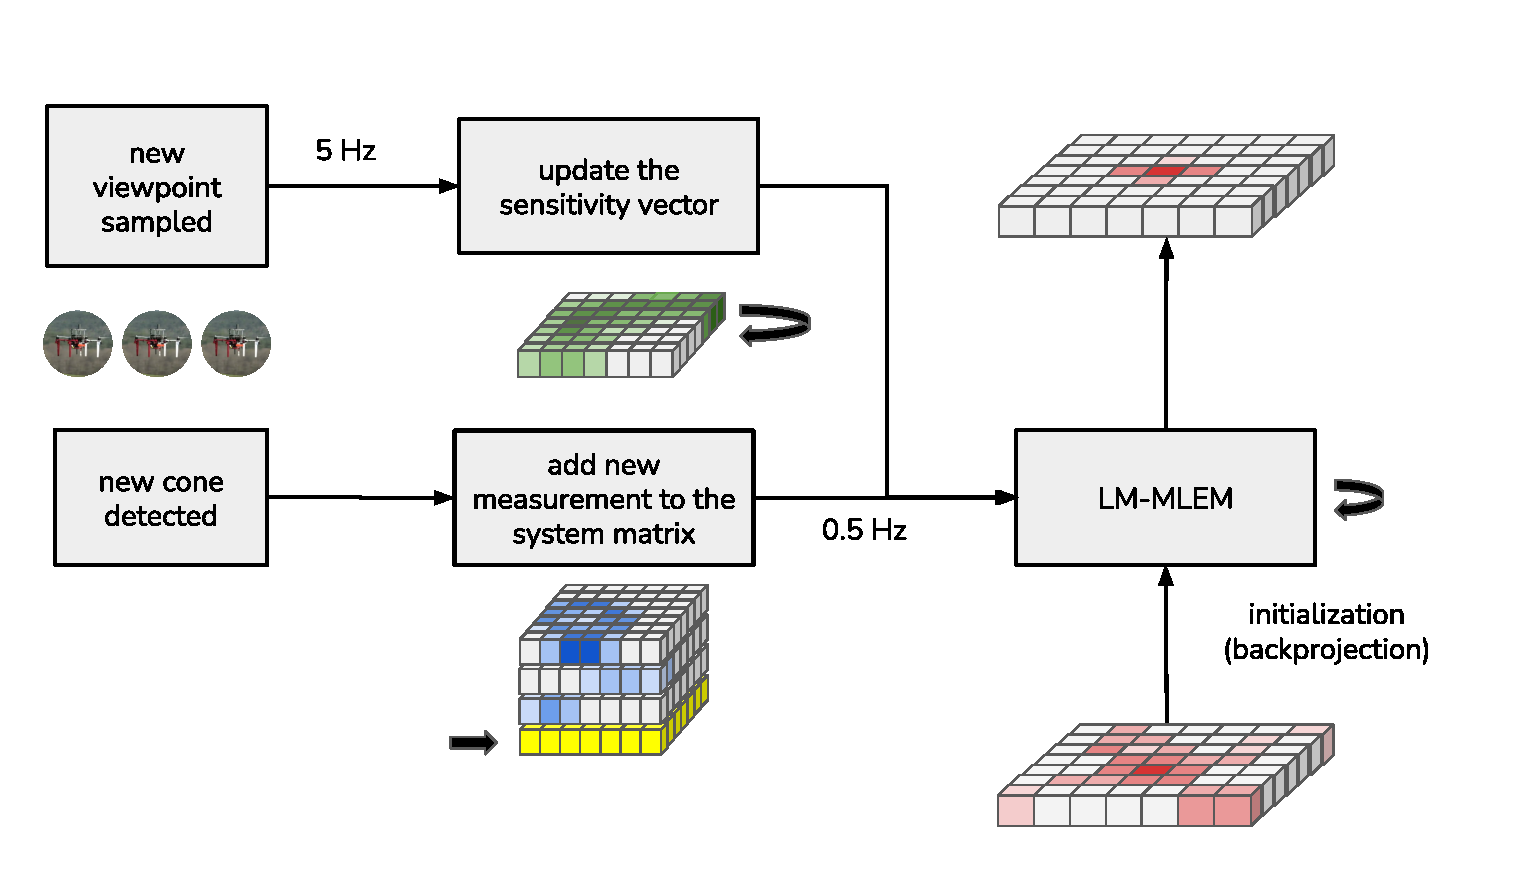
\includegraphics[width=0.99\textwidth]{./fig/photos/online_estimation.eps}
  \caption{Workflow of online \ac{MLEM} estimation.}
    \label{fig:online_mlem}
\end{figure}% %%}

\section{Sensitivity of detection}% %%{
\label{sec:sensitivity}
The probability of a photon emitted from a given position $j$ to be detected by the compton camera is called sensitivity of detection.
It can be expressed using conditional probability as 
\begin{equation}
  s_{j} =  P(\textrm{detected by the sensor}\ | \textrm{emitted from } j).
\end{equation}

A series of random occurrences should happen for a photon to be detected by the compton camera.
First of all, the photon must be emitted from position $j$ towards the sensor surface (emitted under the solid angle subtended by the visible camera surface at the position of the source), not being absorbed by the air along the way.
Then the photon should interact with the matter of the sensor in form of compton scattering.
The angle under which it scatters is described by the Klein-Nisnina cross section.
The scattered photon then must be absorbed by the camera in form of a photoelectric effect.
This model is simplified, because other random occurrences might happen - for example the photon might undergo \ac{CS} twice in a row, the sensor might not detect the interations properly, etc.
However, we will stick to the proposed simplified model with particles undergoing \ac{CS} and then \ac{PE} interactions consecutively.

The literature describes several analytical models for computing sensitivity of the detection. 
For example \cite{wilderman2001} proposed sensitivity model for multi-layer compton cameras in the close distance to the source.
\cite{maxim2016} proposed simplified model for comptom-cameras with negligible size compared to the distance from the source.
However, these models are not suitable for the problem tackled in this thesis.
The multi-layer compton camera has different properties then single-layer sensor \ac{pix}.
Multi-layer compton cameras are typically measuring only particles coming from certain directions (from the front side of the camera, perpendicular to its layers).
On the other hand, the \ac{pix} sensor used in this project can potentially measure particles coming from all directions.
The sensitivity of the sensor w.r.t. different directions of the incoming particle is unknown and present a scientific question, that needs to be answered to make the \ac{LM-MLEM} working. 

Another option presented in literature is evaluation of sensitivity using the Monte-carlo simulation.
This approach has multiple advantages: it is not necessary to describe all random occurrences inside the detector by a single expression (which might take non-negligible computation time when evaluating big number of map positions during the experiment).
Monte-carlo simulation can be precomputed in advance and the data can be stored in some data structure that allows fast access to the data, shortening the computation time.

In our case, the position of the detector is not static. 
The \ac{UAV}s carrying the compton camera are dynamically moving through the environment, with varying speed, position and orientation.
Therefore, the positions of the \ac{UAV}s are sampled in time from \ac{UAV}s trajectories and denoted as $v$, where $v \in (0, \dots , V)$ and $V$ is the total number of viewpoints generated by all \ac{UAV}s during the experiment.
The sensitivity of detection is evaluated for each $jv$ pair. % %%}
%figure sensitivity%%{
\begin{figure}[!h]
  \centering
    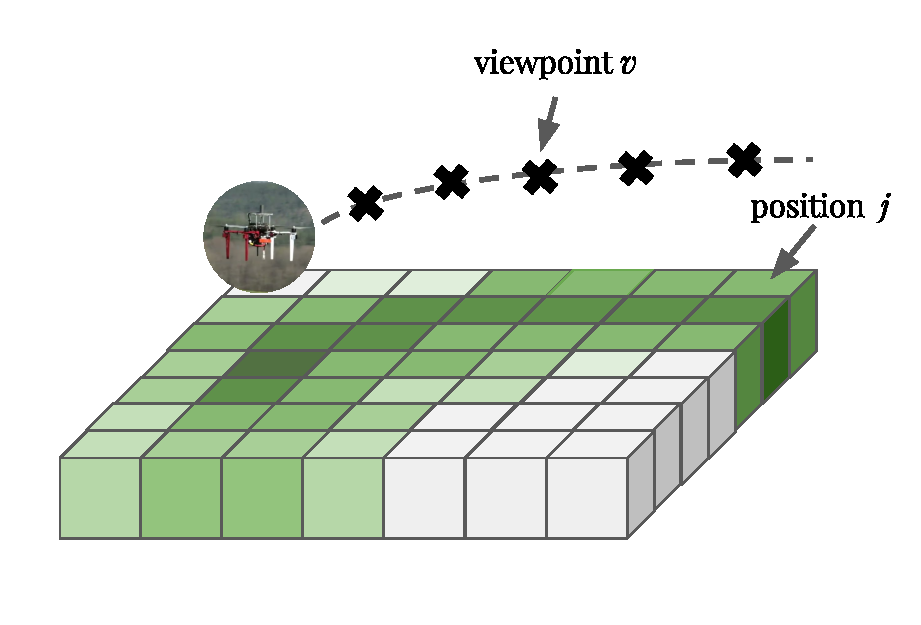
\includegraphics[width=0.6\textwidth]{./fig/photos/sen.eps}
    \label{fig:sen_illustration}
  \caption{An illustration of sensitivity computation. Sensitivity describes probability that particle emitted at given position is measured by the compton cameras onboard the \ac{UAV}s. In other words, it describes how well explored is given map position during the experiment. The trajectory of the \ac{UAV} is sampled into viewpoints denoted as $v$.}
\end{figure}% %%}

\subsection{Probabilistic description}% %%{
The series of random occurrences for a photon emitted at position $j$ leading to the detection by the compton camera at camera position $v$ can be described as follows:
\begin{equation}
  s_{jv} =  (p_{solid\ angle})(1-p_{air})(p_{compton})(p_{absorption}),
  \label{eq:sen_prob}
\end{equation}
where $p_{solid\ angle}$ is the probability that photon is emitted towards the solid angle of the surface of the detector visible from source position, 
$p_{air}$ is the probability that photon is absorbed by the air along the way from emission towards the sensor, 
$p_{compton}$ is probability that Compton scattering occurs and $p_{absorption}$ denotes that scattered photon is absorbed by the detector and measured.

It is difficult to describe  equation \ref{eq:sen_prob} for \ac{pix} Compton camera in analytical form since the probability $p_{compton}$ and $p_{absorption}$ depends on the length of corresponding intersection of the photon's trajectory with the matter of the detector.  
However, it is possible to simulate high number of particles and approximate the terms $(p_{solid\ angle})$, $(p_{compton})$ and $(p_{absorption})$ using a Monte-carlo simulation.% %%}

\subsection{Monte Carlo simulation}% %%{
The idea of Monte Carlo simulation is simple:
instead of deriving analytical expression,
which might be complicated given the nature of the \ac{pix} detector (where all interactions are happening in a single block of matter and probabilities of \ac{CS} or \ac{PE} depend on the length of the ray segment inside the sensor) and time-consuming for online computations during the experiment,
we will place simulated sources at certain position and compute how many particles produced Compton cones in the simulated sensor.
The realistic Compton camera simulator described \cite{baca2019timepix} was used as a template and adapted for this particular application.

%Figure \ref{fig:polar} shows the polar coordinate system, where angles $\theta$ and $\phi$ determines the relative position of the source with respect to the compton camera.
Position of each simulated source is parametrized by its polar coordinates (angles $\theta$ , $\phi$ and distance $d$), as shown in figure \ref{fig:polar}.
Each simulated source emits $N$ particles (in all directions).
Since the \ac{CdTe} sensor's block is a symmetrical object, only $\frac{1}{8}$ of the elementary sphere around the sensor needs to be simulated.
Figure \ref{fig:sources_loc} shows the positions of simulated sources and figure \ref{fig:sampling} presents their positions in the angle space.
We compute the probability of producing a Compton cone for particle emitted by a source at relative position given by polar coordinates ($\theta, \phi, d$) as
\begin{equation}
  p(\mathrm{cone\ detection})_{(\theta, \phi, d)} = \frac{C_{(\theta, \phi, d)}}{N},
\end{equation} 
where $C_{(\theta, \phi, d)}$ is the number of particles that undergone \ac{CS} and \ac{PE} consecutively inside the Compton camera and passed the outlier detection (therefore can be detected).
The outlier detection consists of minimum pixel distance of the two recorded interactions on the Timepix chip and energy bounds for recorded electron with energy $E_{1}$ and photon $E_{2}$. 
$N$ is the number of all particles emitted at source position $(\theta, \phi, d)$. 
Number of emitted particles is set to $N = 10^{10}$, the distance $d$ is set to $d = \SI{1}\meter$.
The simulation process is described in algorithm \ref{alg:monte}. 
The results of the simulation are stored in a lookup table:
\begin{equation}
  \mathrm{lookup\_table}(\theta_{k}, \phi_{k}) = p(\mathrm{cone\ detection})_{(\theta_{k}, \phi_{k}, d = \SI{1}\meter)}. 
\end{equation}
It is a data structure that allows fast readout of the stored data.
For arbitrary query ($\theta, \phi$) it finds the closest key pair ($\theta_{k}, \phi_{k}$) in the angle space and returns its value.% %%}

%multifigure montecarlo
\begin{figure}[!h]% %%{
  \centering

  \subfloat[\centering Polar coordinates] {
    \centering
    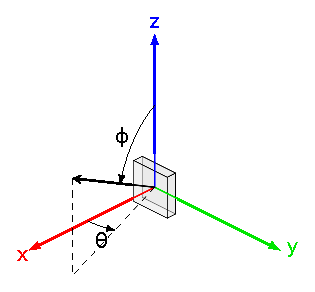
\includegraphics[width=0.3\textwidth]{./fig/photos/axes.eps}
    \label{fig:polar}
  }
  \subfloat[\centering Locations of the simulated sources] {
    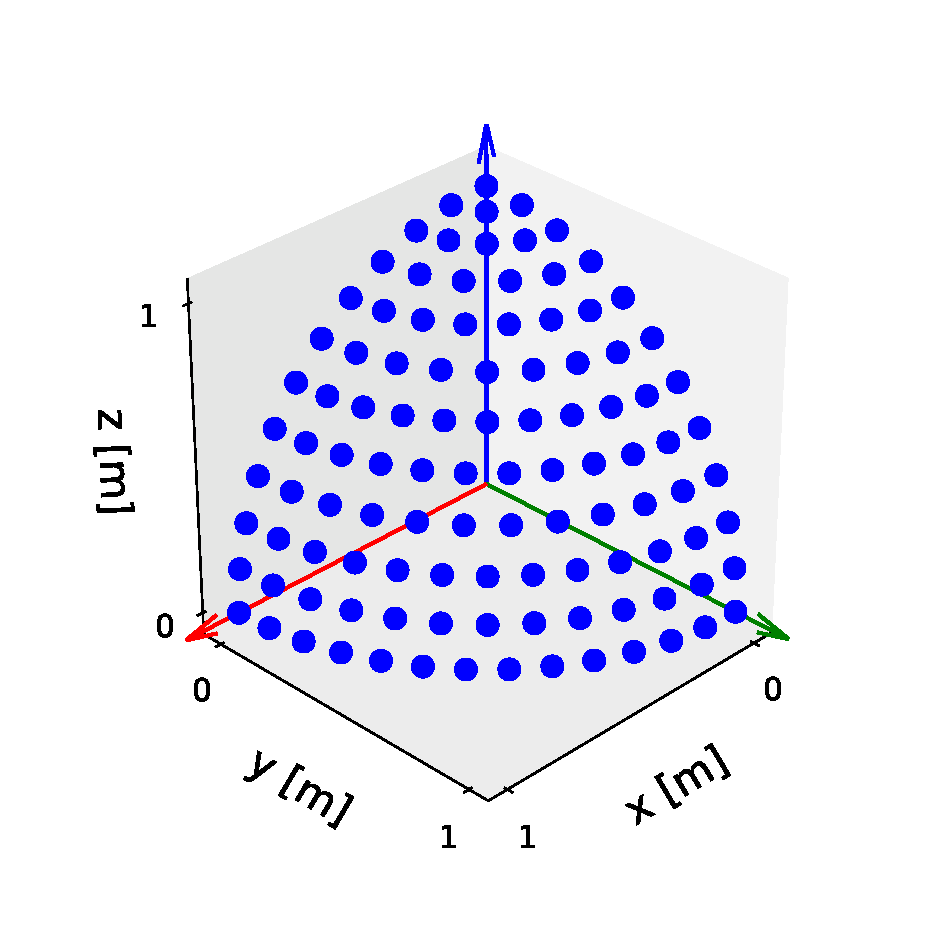
\includegraphics[width=0.33\textwidth]{./fig/photos/mc_sources.eps}
    \label{fig:sources_loc}
  }
  \subfloat[\centering Sampling of the $\frac{1}{8}$ of the unit sphere in the angle space] {
    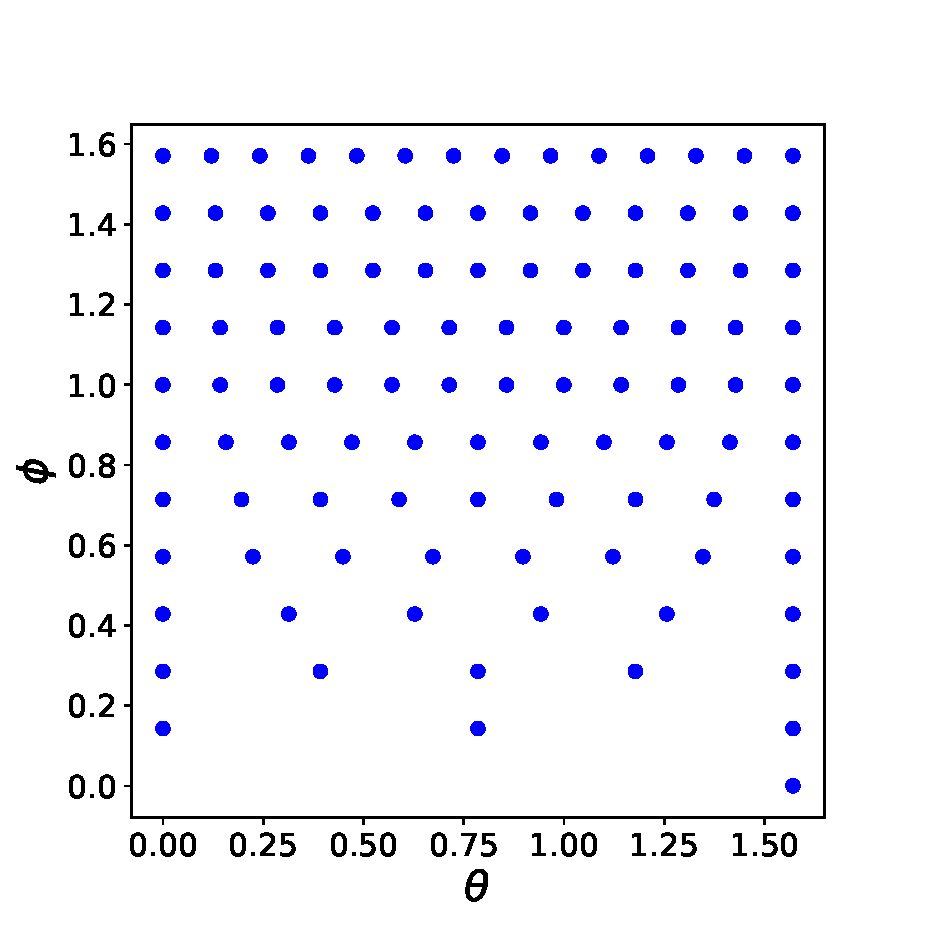
\includegraphics[width=0.33\textwidth]{./fig/photos/mc_angle_space.eps}
    \label{fig:sampling}
  }
  \caption{}
  \label{fig:mc_multi}
\end{figure}% %%}

%%%%%%%%%%% ALGORITHM %%%%%%%%%%%%%%%%%% %%{
%%%%%%%%%%%%%%%%%%%%%%%%%%%%%%%%%%%%%%%%%%%
\begin{algorithm}[h!]
\caption{Monte-carlo simulation}\label{alg:cap}
\begin{algorithmic}
\Function {create\_lookup\_table}{$N$}
  \For {$\theta \in (0, \dots ,\frac{\pi}{2})$}
    \For {$\phi \in (0, \dots , \frac{\pi}{2})$}
      \State $\mathrm{lookup\_table}(\theta, \phi) \gets \Call{compute\_probability}{\theta, \phi, N}$
    \EndFor
  \EndFor
\EndFunction
\Statex
\Function {compute\_probability}{$\theta, \phi, N$}
\State $C \gets 0$
\State $A \gets N\frac{\Omega_{\theta, \phi}}{4 \pi}$ \Comment{how many of $N$ particles hits the sensor}
\State $a \gets 0$
\While {$a<A$} 
  \If {\Call{is\_cone\_measured}{$\theta, \phi$}} \Comment{Compton cone measured}
  \State $C \gets C + 1 $ 
  \EndIf
  \State $a \gets a + 1$
\EndWhile
  \State \Return $C/N$ 
  \EndFunction
\Statex
  \Function{is\_cone\_measured}{$\theta,\phi$}
  \State $ray \gets \Call{sample\_sensor\_surface}{\theta,\phi}$ \Comment{ray inside the sensor after hitting its surface}
  \If{\Call{is\_Compton\_scattering}{$ray, E_{0}$}} \Comment{sample if \ac{CS} occured}
  \State $new\_ray, E_{1}, X_{1} \gets \Call{compton\_scattering}{ray, E_{0}}$ %\Comment{Sample }
  \Else{}
    \State \Return False \Comment{No Compton scattering occurred}
  \EndIf
  \If{\Call{is\_photoelectric\_effect}{$new\_ray, E_{1}$}} \Comment{Sample if \ac{PE} occurred} 
    \State $E_{2}, X_{2} \gets $\Call{photoelectric\_effect}{$new\_ray, E_{1}$}
  \Else{}
    \State \Return False
  \EndIf
  \If{\Call{passed\_outlier\_detection}{$E_{1}, E_{2}, X_{1}, X_{2}$}}  \Comment{pixel dist. and energy bounds}
    \State \Return True   
    \Else{}
    \State \Return False
  \EndIf
\EndFunction
\end{algorithmic}
  \label{alg:monte}
  \caption{Monte-carlo simulation}
\end{algorithm}
%%%%%%%%%%%%%%%%%%%%%%%%%%%%%%%%%%%%%%%%%%%% %%}

\subsection{Sensitivity vector definition}% %%{
The sensitivity of detection by the sensor placed at sampled position $v$ for map position $j$ is computed as:
\begin{equation}
  s_{jv} = \underset{(1-p_{air})}{\underbrace{e^{-((\mu/\rho) d_{jv})} }} \underset{(p_{solid\ angle})\\(p_{compton})\\(p_{absorption})} {\underbrace{\frac{\mathrm{lookup\_table}(\phi_{jv}, \theta_{jv})}{d^{2}_{jv}}}},  
  \label{eq:sjv}
\end{equation}
where $d_{jv}$ is the euclidean distance between map position $j$ and sensor position $v$, ($\mu/\rho$) is the total attenuation coefficient for air (based on \cite{nist}), ($\phi_{jv}, \theta_{jv}$) are polar coordinates determining the relative position of $v$ and the sensor. 
The term $\frac{1}{d^{2}_{jv}}$ in \ref{eq:sjv} ensures that the $p_{solid\ angle}$ (already contained in the $\mathrm{lookup\_table}$ for $d = \SI{1}\meter$) approximately holds even for distances other than $d = \SI{1}\meter$.

\subsection{Iterative formula}
The equation \ref{eq:sjv} presents the sensitivity computation for one viewpoint $v$. 
It is required to compute the sensitivity of detection online during the experiment for all the viewpoints from all \ac{UAV}s sampled so far. 
Therefore it is iteratively updated with the new sampled viewpoints (\ac{UAV} positions).
Let denote $\mathbf{S}^{[n]}$ the sensitivity matrix at update step $n$.
The initial value of $\mathbf{S}^{[0]}$ is set to $0$ ($s_{j}^{[0]} = 0 ,\forall s_{j}^{[0]} \in \mathbf{S}^{[0]}$).
Lets denote $V^{[n:n+1]}$ the set of viewpoints that were newly sampled after update step $n$ and needs to be processed. 

The sensitivity matrix $\mathbf{S}^{[n+1]}$ with elements $s_{j}^{[n+1]}$ is computed as follows:
\begin{equation}
  s_{j}^{[n+1]} = s_{j}^{[n]} + \sum_{v \in V^{[n:n+1]}} s_{jv} \Delta_{v}, 
  \label{eq:sen_iter}
\end{equation}
where the sum $\sum_{v \in V^{[n:n+1]}}$ iterates over all newly processed viewpoints, 
the term $\Delta_{v} = t_{v} - t_{v-1}$ expresses the time difference between current viewpoint $v$ sampled at time $t_{v}$ and its predecessor (previous viewpoint generated from the trajectory of the same \ac{UAV}) sampled at time $t_{v-1}$. 

This formulation of sensitivity has multiple advantages.
Firstly, the memory requirements for storing the matrix $\mathbf{S}$ remain the same during the whole experiment, the values $s_{j}$ are updated in place.
Secondly, the sensitivity is updated online as new sampled trajectories of the \ac{UAV} arrive, therefore the computation time scale well with increasing duration of the experiment.
Lastly, it takes into account the time difference between sampled viewpoints $\Delta_{v}$.% %%}

%%%%%%%%%%%%%%%%%%%%%%%%%%
%%%%%%%%%%%%%%%%%%%%%%%%%%
%%%%%%%%%%%%%%%%%%%%%%%%%%
\section{System matrix}
\label{sec:system}
The system matrix $\mathbf{T} \in \mathbb{R}^{I \times J}$ is defined as
\begin{equation}
t_{ij} =  P(\textrm{detected in } i | \textrm{emitted from } j).
\end{equation}
In other words, it says how likely the photon causing measurement $i$ came from the map position $j$.
The illustration of the system matrix is depicted in figure \ref{fig:sys_ilustration}, where the blue color represents $t_{ij}$ values of the individual cells. 
\begin{figure}[!h]
  \centering
    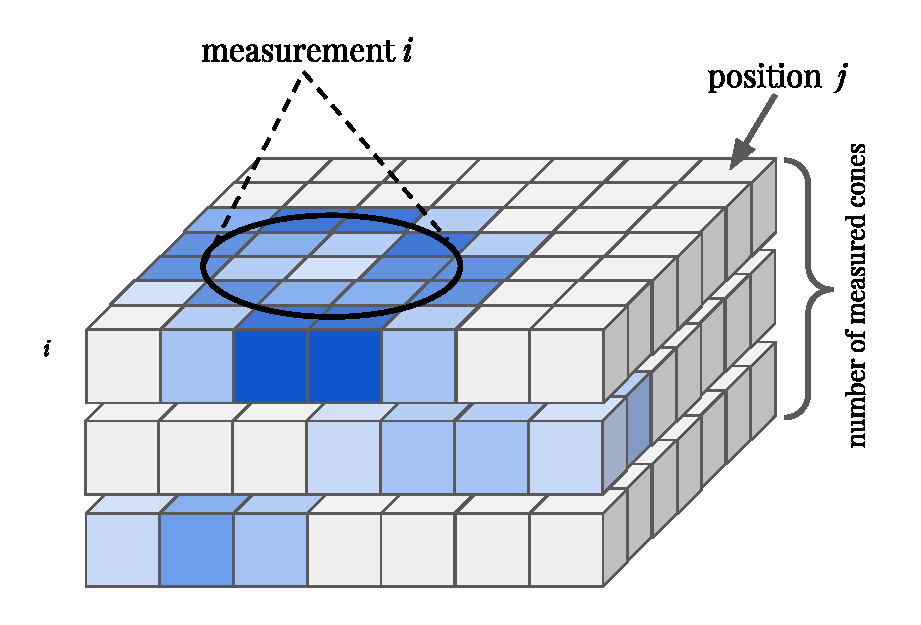
\includegraphics[width=0.48\textwidth]{./fig/photos/sys.eps}
  \caption{System matrix $\mathbf{T}$. The blue color represent the value of $t_{ij}$ in each cell.}
    \label{fig:sys_ilustration}
\end{figure}

%The main question remains the same as for the sensitivity computation: how to evaluate the system matrix for given scenario and \ac{pix} sensor?

The measurement $i$ is composed of multiple components:
\begin{equation}
  i_{full} = (\beta_{i}, v_{i}, a_{i}, X_{1}, E_{1}, X_{2}, E_{2}),
\end{equation}
where:
\begin{itemize}
  \item $\beta_{i}$ is the reconstructed Compton angle,
  \item $v_{i}$ is the 3D pose (position and orientation) of the sensor in world coordinates at the time when the event was recorded,
  \item $\mathbf{a}_{i}$ is the axis vector of the reconstructed Compton cone,
  \item $X_{1}$ is the position of first interaction (Compton scattering) inside the detector,
  \item $E_{1}$ is the measured energy of the electron that was created as side product of the Compton scattering,
  \item $X_{2}$ is the position of the second interaction (absorption) inside the detector,
  \item $E_{2}$ is the measured energy of the absorbed electron.
\end{itemize}
%The first interaction (electron produced as a side product of \ac{CS}) at position ${X_{1}}$ with measured energy $E_{1}$) 
%and the second interaction (absorbed electron at position $X_{2}$ inside the sensor with measured energy $E_{2}$).
%The Compton cone $i$ with scattering angle $\beta_{i}$ is then reconstructed from these measurements using equation \ref{eq:theta}.
%The position of the sensor at the time when the Compton effect was measured is denoted $v_{i}$ (and is composed of position and orientation in the world coordinates).

\subsection{Probabilistic description}
A series of random occurrences should happen for a photon emitted at position $j$ with initial energy $E_{0}$ to be detected by the Compton camera as measurement $i$.
it can be described with probabilities as:
\begin{itemize}
  \item $p_{solid\ angle}(j, v_{i}) $ - probability that the photon is emitted at position $j$ under the right solid angle towards the visible surface of the detector at position $v_{i}$,
  \item $(1-p_{air}(d_{jv_{i}}))$ - probability that the photon reach the detector surface (not being absorbed along the way, where $d_{jv_{i}}$ is the distance from $j$ to detector pose $v_{i}$),
  \item $\bar{p}_{compton}(j, X_{1}, E_{0}, \beta_{i})$ - probability that it interacts with the matter of the detector at position $X_{1}$ and undergo Compton scattering under angle $\beta_{i}$, while loosing energy $E_{1}$ to the electron that is immediately measured by the detector,
  \item $\bar{p}_{absorption}(X_{1}, X_{2}, E_{0}, E_{1})$ - probability that the scattered photon interacts with the matter of the detector at position $X_{2}$, is absorbed and energy $E_{2}$ is measured by the detector during the absorption.
\end{itemize}
Same as in sensitivity section, the presented model is simplified and several assumptions are made. 
It is assumed that the first interaction is a Compton scattering and the second interaction is photoelectric effect (absorption) (which might not be always true, since other interactions might occur), it is assumed that $E_{0} = E_{1} + E_{2}$, etc.
Unlike in sensitivity computation (where $s_{j}$ describes probability that photon emitted from $j$ is detected anywhere by the detectors), the elements of system matrix $t_{ij}$ describes probability that a photon emitted from $j$ was recorded in measurement $i$, therefore $p_{compton}\neq \bar{p}_{compton}$ and  $p_{absorption}\neq \bar{p}_{absorption}$.

\subsection{Inspiration in literature}
The nuclear medicine literature provides multiple models for the system matrix, such as \cite{wilderman}. 
However, the model is designed for two-layer \ac{CC} and for scenarios where the detector size is relatively large compared to the distance to the source and therefore the geometry of the \ac{CC} must be considered.
Work presented in \cite{maxim2016} described simplified model for \ac{CC} which size is negligible compared to the distance to the source of radiation (for two-layer \ac{CC}).
The energy measurement uncertainties are approximated using gaussian distribution.
Both of these models do not take into account the effect of environmental attenuation.
Despite all of these differences, it served as an inspiration for the proposed approach.

\subsection{Simplifications}
Efficient evaluation of $\bar{p}_{compton}$ and $\bar{p}_{absorption}$ is challenging since it depends on the length of the incoming and scattered ray inside the detector.
In the given scenario, the size of the \ac{pix} detector is negligible ($14 \times 14 \times 2 \ \mathrm{mm}$) compared to the distance between the detector mounted on the \ac{UAV} (flying at least $\SI{3}\meter$ above the ground) and source of radiation.
Because of that, modelling $p_{solid\ angle}$ (probability that the particle reaches the detector) and $p_{air}$ (air attenuation) is relatively more important than the accurate modelling of probabilities of events inside the detector.

The following simplification is made:
The measurement $i$ is represented as
\begin{equation}
  i = (\beta_{i}, v_{i}, a_{i})
\end{equation}
and the measured energies and exact positions of interactions inside the detector are ignored,
the \ac{CC} detector is approximated as a single point with position and orientation $v_{i}$.
However, the probability of detecting Compton effect produced by particle incoming from some direction is not uniform for all directions (given the non-uniform shape of the sensor).
The lookup table from previous section (representing the chance that particle incoming from specific direction cause any detectable Compton effect, not just the one measured in $i$) is used to approximate the direction sensitivity of the detector.
\begin{figure}[!h]
  \centering
    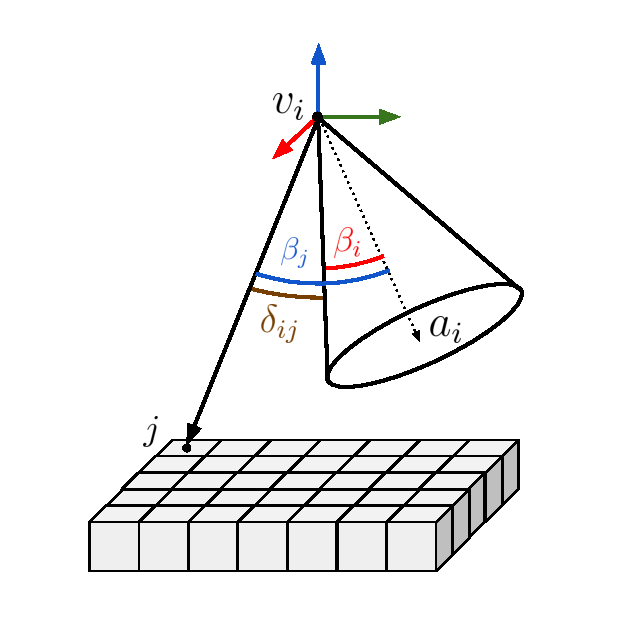
\includegraphics[width=0.4\textwidth]{./fig/photos/system_comp.eps}
    \caption{An illustration of the measurement $i$, which is composed of cone origin $v_{i}$, axis vector $a_{i}$ and Compton angle $\beta_{i}$.}
    \label{fig:system_comp}
\end{figure}

\subsection{System matrix definition}
The elements $t_{ij}$ of system matrix $\mathbf{T}$ are computed as:
\begin{equation}
  t_{ij} = \underset{(1-p_{air})}{\underbrace{e^{-((\mu/\rho) d_{jv_{i}})}}}\ 
  \underset{\bar{p}_{compton}} {  \underbrace{K(\beta_{i}, E_{0})\ h(\delta_{ij}|\sigma, \alpha_{ij})}} \
  \underset{(p_{solid\ angle})\\(p_{compton})\\(p_{absorption})} {\underbrace{\frac{\mathrm{lookup\_table}(\phi_{jv}, \theta_{jv})}{d_{jv_{i}}^{2}}}}
  ,%s_{jv} = \underset{(1-p_{air})}{\underbrace{e^{-((\mu/\rho) d_{jv})} }} \underset{(p_{solid\ angle})\\(p_{compton})\\(p_{absorption})} {\underbrace{\frac{\mathrm{lookup\_table}(\phi_{jv}, \theta_{jv})}{d^{2}_{jv}}}},  
  \label{eq:system_matrix_full}
\end{equation}

where:
\begin{itemize}
 \item $d_{jv_{i}}$ is the euclidean distance between the map position $j$ and sensor position $v_{i}$, 
\item ($\mu/\rho$) is the total attenuation coefficient for air (based on \cite{nist}),
\item $K(\beta_{i}, E_{0})$ is the Klein-Nishina formula representing probability of Compton scattering under estimated angle $\beta_{i}$ for incoming particle with energy $E_{0}$,
\item $h(\delta_{ij}|\sigma_{j})$ is a gaussian kernel (the "blurring factor") representing the uncertainty in angle measurement,
\item $\delta_{ij}$ is angle difference $|\beta_{i}-\beta_{j}|$, where $\beta_{j}$ is the angle between cone axis vector $a_{i}$ and vector $|j-v_{i}|$, 
\item $\sigma$ is standard deviation and $\alpha$ is the minimal angle difference due to discretization noise,
\item $\mathrm{lookup\_table}(\phi_{jv}, \theta_{jv})$ is the lookup table defined in section \ref{sec:sensitivity}.
\end{itemize}

The angular difference $\delta_{ij}$ in equation \ref{eq:system_matrix_full} comprise the measured Compton cone.
If the reconstructed Compton cone (with origin $v_{i}$, axis vector $a_{i}$ and Compton angle $\beta_{i}$) would perfectly intersects the map position $j$, then the angular difference would be $\delta_{ij} = 0$, as illustrated in figure \ref{fig:system_comp}.
However, this holds only for perfect world without noise.

\subsubsection{Measurement noise}
The real world measurements are affected by measurement noise, hence the reconstructed cone might not intersect the real position of emission.
The measurement noise might be present in the measured energies $E_{1}$ and $E_{2}$ (that are affecting the Compton angle $\beta_{i}$ , see equation \ref{eq:compton_beta_formula}) 
as well as in the positions of interactions inside the detector ($X_{1}$ and $X_{2}$) 
that are affecting the cone axis $a_{i}$.
The influence of noise in energy measurement (Compton angle $\beta$) is modelled using Gaussian function with ``standard deviation'' $\sigma$:
\begin{equation}
  h(\delta_{ij}|\sigma) = e^{-\frac{1}{2}(\frac{\delta_{ij}}{\sigma})^{2}}.
  \label{eq:gau}
\end{equation}
If the angle difference is to big ( $\delta_{ij}<3\sigma$), then $h(\delta_{ij}|\sigma) = 0$.
The important question is how to set the parameter $\sigma$, that is influencing the width of the function \ref{eq:gau}.
The datasheet\footnote{Available at: https://advacam.com/camera/minipix-tpx3}
states that the energy resolution of used \ac{pix} sensor is $4.5 - 9.9\ \mathrm{kEV}$. 
Dependence of angular uncertainties on the energy resolution of two layer Compton cameras was studied in \cite{ordonez}.
The measurement of the energies is not the only source of noise in the detection pipeline.
The $h(\delta_{ij}|\sigma)$ function should disperse the conical back-projections in order to tackle other inaccuracies, such as noise in the sensor's position or wrongly estimated axis of the Compton cone. 
The exact estimation of angular uncertainty (and other sources of noise) is beyond the scope of this thesis.
i%Other sources of noise (such as positions of interaction inside the detector $X_{1}$, $X_{2}$, especially depth of interaction in the sensor block) are difficult to model as well.
For "proof of concept" demonstration, the value $\sigma$ was set empirically based on recorded data from experiments with real \ac{pix} sensors.

\subsubsection{Discretization error}
Another possible source of noise is the discretization of the area of interest, which is divided into $J$ discrete bins (each represented by its center position) with step size $l$.
Even perfectly measured and reconstructed Compton cone might not intersect the real position of emission (meaning $\delta_{ij}$ would be non-zero) due to the discretization of $J$.
Lets define maximal error for measurement $i$ and position $j$ caused by discretization as
\begin{equation}
  \alpha_{ij} = \mathrm{arctan}(\frac{x}{d_{jv_{i}}}),
  \label{eq:alpha}
\end{equation}

where $d_{jv_{i}}$ is the distance between cone origin at position $v_{i}$ and map position $j$ and $x$ is the maximal allowed distance between projected cone and discrete position $j$, $x = l$.
The situation is illustrated in figure \ref{fig:discret}.

\begin{figure}
  \centering
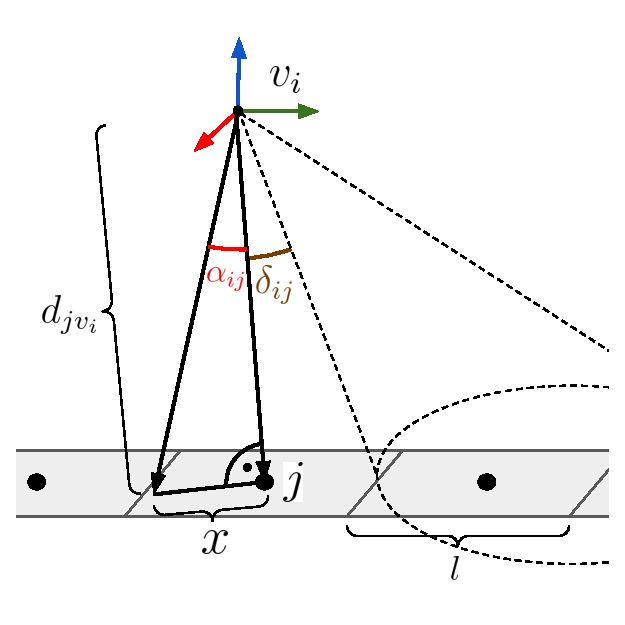
\includegraphics[width=0.4\textwidth]{./fig/photos/discret.eps}
  \caption{Illustration of discretization error. The maximal angle difference caused by discretization error $\alpha_{ij}$ is computed for each map position $j$.}
  \label{fig:discret}
\end{figure}

Taking into account the discretization as well as measurement noise, the term $h(\delta_{ij}|\sigma, \alpha_{ij})$ in equation \ref{eq:system_matrix_full} which is projecting the cone to the map positions is defined as
\begin{equation}
h(\delta_{ij}|\sigma) =
\begin{cases}
1 & \text{if $\delta_{ij}\leq \alpha_{ij}$}\\ 
e^{- \frac{1}{2}(\frac{\delta_{ij}}{\sigma})^{2}} & \text{if $\delta_{ij} > \alpha_{ij}$ and  $\delta_{ij} \leq 3\sigma_{j}$} \\
0 & \text{otherwise}
\end{cases}, 
\end{equation}
where $\alpha_{ij}$ is the maximal angle difference caused by discretization error defined in equation \ref{eq:alpha}.





\mycomment{% %%{
    \section{Preliminaries}
    %Localization of multiple sources of ionizing radiation using a group of \ac{UAV}s equipped with Compton cameras \ac{pix} is a challenging task for several reasons.
    The nature of radioactive emission (as well as the detection and reconstruction process) make the localization of sources of ionizing radiation a challenging task.
    The following main problems were encountered during the work on this thesis:
    \subsection{Observed challenges in localization of multiple radioactive sources}
    \subsubsection{Measurement - position dependency}
    As described previously, the sensing range of ionizing radiation detectors is limited due to the fact that the intensity of radiation decreases with distance (following the inverse square law).
    The initial experiments with pre-recorded data from real experiments as well as method proposed in \cite{baca2021gamma} showed that it results into position-measurement dependency, where the quality of measurements heavily depends on the traversed trajectories of the \ac{UAV}s.

    Imagine following scenario:
    there are two sources of ionizing radiation $A$ and $B$.
    Both have the same emission activity (average number of particles emitted per second).
    The is an \ac{UAV} equipped with Compton camera, that is traversing the area.
    It can either traverse the whole area following some predefined pattern (hence cover the space uniformly), which might be slow and inefficient.
    The second option is to traverse the space using arbitrary trajectories, which might lead to faster execution time.
    However, since the coverage of the area is not uniform, the drone could fly above the source $A$ more times than above the source $B$.
    It means that it measured more $\gamma$ particles above source $A$, although both sources have the same emission activity.

    This observed phenomena is generally not desired.
    It would be nice to not only localize the sources, but also estimate their (absolute, or at least relative) emission activity.
    In ideal world, the estimation method should be able to mitigate this effect.
    The quality of estimate of sources distribution should be as independent on the \ac{UAV} trajectories as possible (given the recorded events).

    \subsubsection{Nature of Compton measurements}
    The detection and reconstruction process for Compton camera allows us to deduce set of possible sources of such particle.
    The set is a surface of the Compton cone.
    It poses a challenge when multiple sources of radiation are present:
    it is impossible to deduce from which source the particle was emitted, since the source could be anywhere on the conical surface.
    Therefore it is not known if the $\gamma$ photon originated from already localized source, or it was emitted elsewhere from some yet unobserved source.
}% %%}


\mycomment{% %%{
  \chapter{Mlem Theory medicine}
  \section{Inspiration in medicine}
  The problem of reconstructing 3D positions of sources of ionizing radiation has been studied in depth in the field of medical imagining.
  To give an example: one possible application of such methods is a cancer diagnostics.
  A small amount of radioactive substance (called tracer) is injected into the patient's vein.
  The tracer is absorbed by different parts of the body in varying amounts, which can show areas with abnormal metabolic activity, which is usually the case for cancer cells.
  The detection of emitted particles and 3D reconstruction of their sources will allow the doctors to find the location of the tumor in the patient's body.

  There are numerous methods used in medical imagining. 
  Two main approaches are following: \ac{PET} and \ac{SPECT}.
  \ac{PET} imagining typically use a gamma emitting radioisotope as a tracer.  
  The method is based on positron emission. 
  The emitted positron interacts with electron in the patients body and both particles vanish in a burst of energy. 
  This energy comes in a form of two gamma rays, that goes into a opposite directions.
  Detection of these two gamma rays (measured by the camera at the same time) allows us to reconstruct 3D image of the patient's body.
  In \ac{SPECT}, single gamma ray is produced. 
  The reconstructed image is computed from gamma rays detected by the camera.
  Since only one gamma-ray is emmited (unlike in \ac{PET}), high number of measurements is needed for accute reconstruction.
  Medical \ac{SPECT} imagining cameras typically use collimators to get some information about direction of incoming gamma ray.
  Collimators restricts the set of possible directions from which the gamma ray may enter the detector (and be detected), therefore they can improve accuracy of the detection.

  Another type of sensor (that can be used in \ac{SPECT} imagining) is a Compton camera.
  The biggest benefit of compton camera is that it provides information about the direction of detected incoming gamma ray without the use of collimator.
  The nuclear medicine reconstruction method for compton camera measurements that served as inspiration for for this thesis is called \ac{LM-MLEM}.

  \section{Maximum likelihood expectation maximization}



  \cite{1982_shepp_vardi_MLEM} \cite{EM} \cite{wilderman}

  \subsection{Maximum likelihood estimation}
  \ac{MLE} is a classical approach in machine learning.
  It is used to estimate the parameters of a probability distribution based on observed data. 
  The goal of \ac{MLE} is to find the parameter values that make the observed data most probable under the assumed probability distribution.
  This is done by calculating the likelihood function, which is the probability of the observed data given a set of parameter values.
  Likelihood can be defined as 
  \begin{equation}
    likelihood = p(\ \mathrm{observations } \  \boldsymbol{O} | \ \mathrm{hidden \ parameters\ } \Phi ).
    \label{eq:likelihood}
  \end{equation}
  We want to maximize this expression with respect to the hidden parameters.
  In other words, we want to find such parameters so that they fit our observations in the best possible way.

  \section{Algorithm formulation}
  Let's divide the area of possible sources of radiation into $J$ discrete bins (indexed with $j$, where $j = 1 \dotsc J$).
  Each discrete bin is represented by its center position.
  Suppose we have measurements divided into $I$ discrete bins indexed with $i$, $i = 1 \dotsc I$.
  The vector $\mathbf{Y}$ with elements $y_{i}, i \in (1, \dots I)$ denotes the number of particles detected in the corresponding bin $i$.
  Let's define matrix $\mathbf{T}$ ($\mathbf{T} \in \mathbb{R}^{I \times J}$), where each position in the matrix is defined as

  \begin{equation}
    t_{ij} =  P(\textrm{detected in } i | \textrm{emitted from } j).
  \end{equation}

  In other words, $t_{ij}$ represents a probability that we observe observation $i$ given the fact that the radioactive particle was emitted from position $j$.

  Let's assume that the number of photons emitted from one position $j$ is a discrete random variable that follows a Poisson distribution with expected value $\lambda_{j}$.
  Our goal is to estimate $\mathbf{\Lambda}$, which has elements $\lambda_{j}$, each corresponding to the expected number of photons emitted from the position $j$.

  The likelihood of measuring $y_{i}$ particles in the measurement bin $i$ w.r.t. $\mathbf{\Lambda}$ can be expressed as (Poisson distribution):
  \begin{equation}
    p(y_{i} |\mu_{i} ) = e^{-\mu_{i}} \frac{\mu_{i}^{y_i}}{y_{i}!},
  \end{equation}
  where $\mu_{i} = \sum_{j} t_{ij}\lambda_{j}$ denotes the average number of events measured in bin $i$.

  The likelihood of all the measurements is
  \begin{equation}  
    p(\mathbf{Y} | \mathbf{T\Lambda} ) = \prod_{i} e^{-\mu_{i}} \frac{\mu_{i}^{y_i}}{y_{i}!}.
  \end{equation}

  After taking its logarithm, we have the following:

  \begin{equation}  
    \mathrm{log}\ p(\mathbf{Y} | \mathbf{T\Lambda} ) = \sum_{i}\left ( -\sum_{j} t_{ij}\lambda_{j} + y_{i} \mathrm{log}(\sum_{j} t_{ij}\lambda_{j})  - \mathrm{log}(y_{i}!) \right ).
    \label{eq:likelihood1}
  \end{equation}
  However, equation \ref{eq:likelihood1} doesn't give an answer to our question - how to determine $\mathbf{\Lambda}$. The solution is to use an iterative \ac{EM} algorithm.

  The \ac{EM} algorithm was originally proposed by \cite{EM}. 

  \section{differences}
  Such medical application typically requires high resolution of the reconstructed image.
  The distances between the source and detector are small (tens of centimeters), number of measured events is high (tens of thousands and more).
  The reconstruction process is typically performed offline (all measurements are collected first and then the algorithms process the data), since there is no need for online estimation and the processing of measured data might take non-negligible time.
  The domain of multirobotic radiation mapping has multiple differences compared to the medical field.
  The distance between source and detector is much higher (tens of meters).
  The \ac{UAV}s have limited payload (hence the detector carried on board must be light and compact).
  It results in the fact that the number of measurements is much lower (hundreds-thousands detected compton events).
  Moreover, we would like to reconstruct the sources of ionizing radiation in real time.
  Despite all of these differences, the aim of this work is to adapt such algorithms to our problem.
}% %%}

\mycomment{% %%{
    \section{Requirements}
    \subsection{Multiple sources}
    Main motivation for this thesis is to develop method that would be capable of localizing multiple compact sources of ionizing radiation.
    The positions, number or emission activity emission activity of the sources is unknown.

    negative measurements

    multiple sources

    iterative method


    \section{The algorithm of choice}
    The choice of reconstruction method for the given task (estimation of sources locations from \ac{CC} measurements acquired by a group of \ac{UAV} equipped with \ac{pix} detector) was made under following assumptions.
    The iterative methods are more flexible and can handle noise in the measurements.
    The distance between the source and \ac{CC} onboard the \ac{UAV}s is high and the number of measured events (represented using list-mode approach) is relatively low.
    There is no prior knowledge about the distribution of radioactive sources.
    The \ac{CC} data are represented using list-mode approach.
    \section{The algorithm of choice}
    The choice of reconstruction method for the given task (estimation of sources locations from \ac{CC} measurements acquired by a group of \ac{UAV} equipped with \ac{pix} detector) was made under following assumptions.
    The iterative methods are more flexible and can handle noise in the measurements.
    The distance between the source and \ac{CC} onboard the \ac{UAV}s is high and the number of measured events (represented using list-mode approach) is relatively low.
    There is no prior knowledge about the distribution of radioactive sources.
    The \ac{CC} data are represented using list-mode approach.

    The \ac{MLEM} algorithm described previously serves as an inspiration for the mapping method described in this chapter.
    Despite all the differences between the medical and multirobotic domain, the \ac{MLEM} algorithm was chosen for several reasons.
    First of all, the nature of the measurements (compton cones) is the same as in the medical algorithms.
    Secondly, the classical method of maximization of likelihood of measured data seems to be good choice for the given problem.
    It can take into account factors influencing the measurements (such as air attenuation, properties of the detector and radioactive emission) in the probabilistic way.
    Lastly, the estimation of sensitivity of detection (how likely the particles from given position were measured) can be beneficial, 
    because it can provide information of how much the \ac{UAV}s already explored the area of interest and where to fly to possibly detect undetected sources.
}% %%}

%!TEX root = ../main.tex

\chapter{Multirobot search strategy}

\alertsuccess{Somehow ok}
This chapter presents a multirobot search strategy for a group of \ac{UAV}s equipped with Compton camera for online estimation of sources of ionizing radiation, which is based on the \ac{MLEM} method described in the previous chapter.
First part describes the objectives and requirements for such method.
The whole system is described in the next section, as well as individual components of the system.
\section{Objectives}
%The \ac{MLEM} method proposed in the previous chapter provides the maximum likelihood estimate of the measured data.
%When the number of detected Compton events is low, the maximum likelihood estimation method might suffer of inaccurate 

\subsection{Measure as much data as possible}
As stated before, the emission of $\gamma$ particles as well as the detection of Compton events are stochastic processes.
The intensity of radioactive emission follows the inverse square law, which means that it decreases as the distance from the source increases.
Due to the small size of the detector, large distances between \ac{UAV}s and sources of ionizing radiation, and the fact that only $2\%$ of $\gamma$ particles reaching the detector are detected by the Compton camera (on average), the number of detected events is limited.
The accuracy of the \ac{MLE} method depends on the number of detected Compton events.
If the number of detected cones is low, the \ac{MLE} method might converge to false detections since the particle could originate from any position on the surface of the Compton cone.
To accurately localize the sources of ionizing radiation, the \ac{UAV}s should collect as many measurements as possible.
This requires the \ac{UAV}s to fly as close as possible to the currently most likely source estimates to either confirm or disprove the presence of the radioactive source at the given position.
It is also desired that the drones stay in motion (instead of hovering above the points of interest), since measurements from different angles are beneficial for sources localization.

\mycomment{% %%{
  As stated before, the emission as well as the detection of Compton events are stochastic processes.
  The intensity of radioactive emission decreases with inverse square law as the distance from source grows.
  Because of the small size of the detector, large distances between \ac{UAV}s and sources oinizing radiation and the fact that only $2 \%$ of $\gamma$ particles that reach the detector are detected by the Compton camera, the number of detected events is limited.
  The accuracy of \ac{MLE} method from definition depends on the number of detected Compton events.
  When the number of detected cones is low, the \ac{MLE} method might converge to false detections (since the particle could originated from any position on the surface of Comtpon cone).
  To measure more data, the \ac{UAV}s should collect as many measurements as possible.
  It requires the \ac{UAV}s to fly as close as possible to the currently most likely source estimates to either confirm or disprove the presence of the radioactive source at the given position.
}% %%}

\subsection{Search for unobserved sources of ionizing radiation}
The sensitivity vector $\mathbf{S}$ described in the previous chapter provides information about coverage of each discrete point $j$ in the area of interest.
The autonomous \ac{UAV}s should control their motion in the way that the whole area is covered.
In another words, the minimum value of sensitivity $\mathrm{min}(s_{j})$ among all positions in the search space should be as high as possible to increase the chance of observing sources that were not yet detected.

\subsection{Active search strategy}
There are two general strategies how an area of interest can be explored by a group of autonomous \ac{UAV}s in order to measure data and estimate sources of ionizing radiation - offline and online.
In offline search, the \ac{UAV}s typically follow predefined paths and collect measurements, that are processed all at once after the flight. 
In online search, the estimation process is performed online and the \ac{UAV}s may react accordingly to the current output of the radiation mapping method.
Incorporating the output of the mapping method into the feedback control loop 
might lead to better estimate (since more measurements might be acquired) and fasten the search time.
In general, an active search strategy allows the group of \ac{UAV}s to use its full potential, therefore it is desired for the given task.

\mycomment{% %%{
\subsection{Motivation for mlem}
Neco o tom yze i negativni mereni jsou dulezity
  The emission of $\gamma$ particles as well as the detection of Compton events are stochastic processes.
  Only a small fraction of emitted $\gamma$ particles are detected by the small \ac{pix} sensor located several meters from the radioactive source.
  Moreover, the intensity of radioactive emission decreases with the inverse square law as the distance from the source grows.
  Taking into account also ther properties of the ionizing radiation and the detection process, the acquired measurements are highly dependent on the trajectories of the \ac{UAV}s performing the search mission.
  The \ac{UAV}s might be controlled in two ways: they can either a) follow some trajectory that cover the whole area of interest uniformly or b) the trajectory of the \ac{UAV} is arbitrary and the coverage of the space is not uniform.
  However, it doesn't use the whole potential of small and agile \ac{UAV}s carrying the Compton camera.
  In b) approach, it is required 
}% %%}

\mycomment{% %%{
  \subsection{Centralized vs. decentralized}
  The multirobot systems can be classified into two groups: centralized and decentralized.
  In a centralized approach, a central control unit is responsible for coordinating the actions of all the robots in the network. 
  This centralized system can provide global information to each robot, enabling them to make more informed decisions based on the overall state of the system.
  On the other hand, it is vulnerable to single points of failure and it requires reliable communication between each agent and the central unit.
  In decentralized system, each robot operates independently, making decisions based on local information and communication with other robots in the network. 
  This approach can provide increased fault tolerance and can be more adaptable to changing conditions. 
  However, the lack of a central control unit can make it challenging to ensure that all robots are efficiently working towards a common goal.
}% %%}

\section{System design description}
\subsection{Task specification}
The proposed search strategy is based on the objectives described above - the group of \ac{UAV}s should autonomously explore the area of interest with no previous knowledge about number, activity or position of sources of ionizing radiation and localize such sources as fast as possible.
The operation of the \ac{UAV}s is divided into two main tasks:
\begin{itemize}
  \item \textbf{exploration} - the drones should explore the area of interest and increase the chance that none of the sources of $\gamma$ particles would be unobserved,
  \item \textbf{exploitation} - the drones should exploit positions where \ac{MLEM} mapping method estimated some emission activity to either confirm the hypothesis and collect more measurements or disprove it (=increase accuracy of the estimation).
\end{itemize}

%\subsection{Assumptions}
%It is assumed that 
%a) a communication via wireless network is provided, 
%b) the mission is performed in outdoor environment with no obstacles, 
%c) the sources of ionizing radiation are located somewhere on the ground, that is for simplicity assumed to be a flat plane.

\subsection{Multirobot architecture}
The multirobot systems can be classified into two groups: centralized and decentralized.
In a centralized approach, a central control unit is responsible for coordinating the actions of all the robots in the network. 
This centralized system can provide global information to each robot, enabling them to make more informed decisions based on the overall state of the system.
%On the other hand, it is vulnerable to single points of failure and it requires reliable communication between each agent and the central unit.
In decentralized system, each robot operates independently, making decisions based on local information and communication with other robots in the network. 

\begin{figure}[!htb]
    \centering
    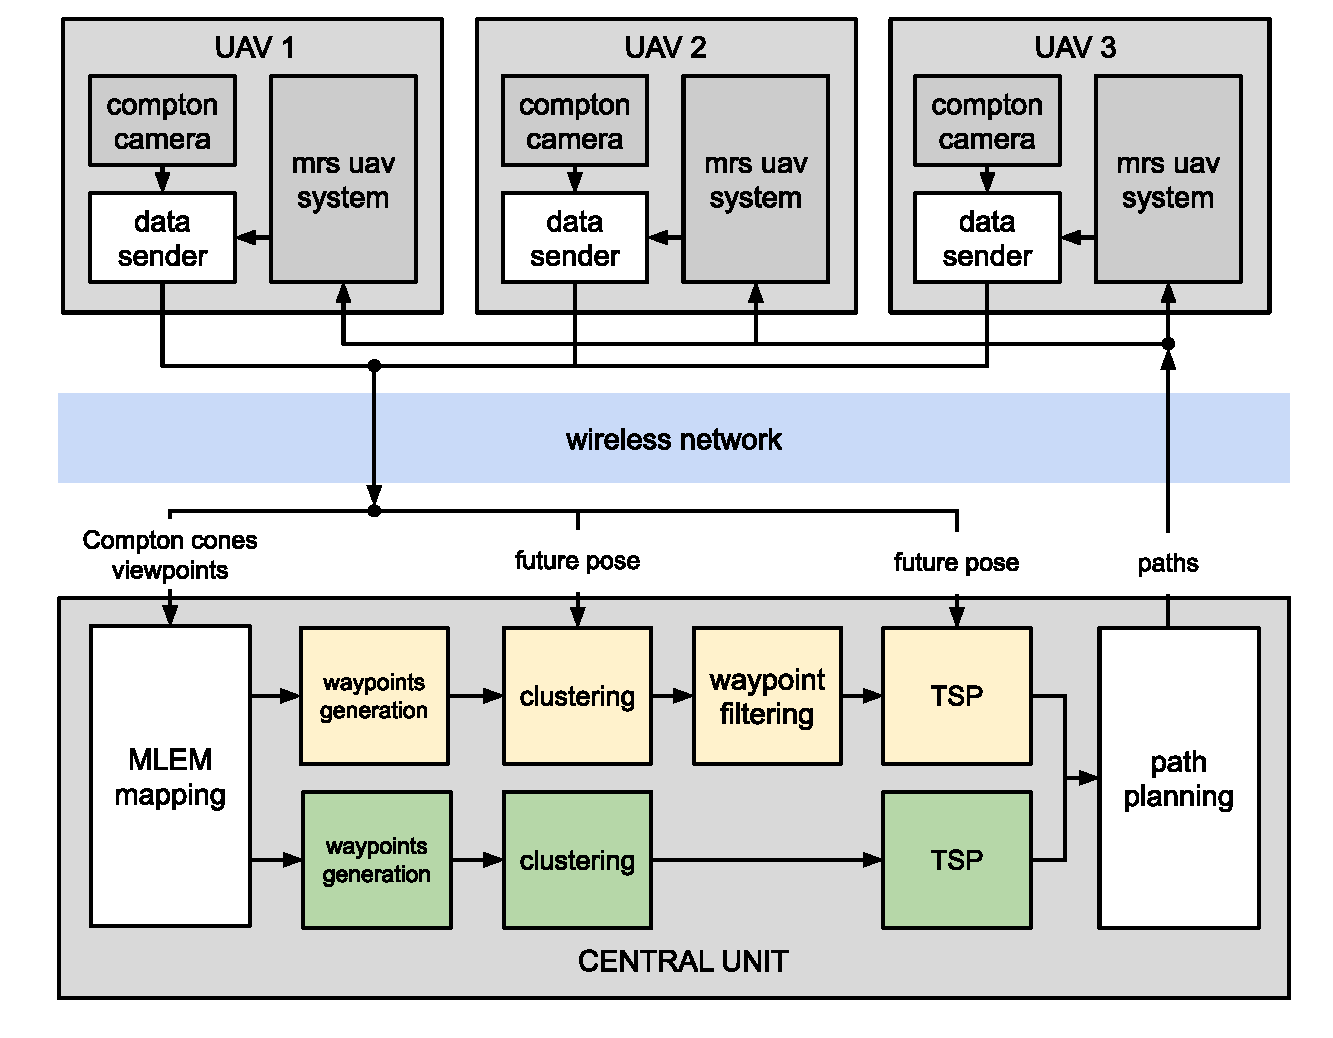
\includegraphics[width=0.99\textwidth]{./fig/photos/system_new.eps}
    \caption{\centering The system architecture diagram. The search and planning method is composed of \ac{MLEM} radiation mapping node, waypoint generation, clustering, waypoint filtering, optimal sequence deduction using TSP and path planning. The exploration (green) and exploitation (yellow) waypoints are processed separately.}
    \label{fig:sysarch}
\end{figure}

The centralized multirobot architecture is used in this project.
The visualization of the system can be seen in figure \ref{fig:pipeline}.
The \ac{UAV}s are communicating via wireless \ac{Wifi} network.
The amount of information shareable via such network is limited.
Therefore all the \ac{MLEM} computations and running on a ground station and the \ac{UAV}s and ground station share the minimal amount of information possible.
All the \ac{UAV}s send its current position and future position in $\SI{2}\second$ as a custom \ac{ROS} message (with frequency $\SI{2}\hertz$), 
together with all newly measured Compton cones.
The ground station processes the measurements and command the \ac{UAV}s by sending non-colliding path for each of them via the wireless network.
The centralized approach have several advantages in this scenario:
The \ac{MLEM} estimate is computed at once, not requiring to share or merge the map with other \ac{UAV}s via the wireless network or run the estimation onboard each drone separately.
The centralized task allocation and path planning is much more straightforward compared to the decentralized approach, where the agents would need to negotiate between each other..
This design choice of course have some disadvantages as well.
The centralized system is vulnerable to single point of failure and the communication between the ground station and all \ac{UAV}s must provided. 

\subsection{Custom data message}
A custom \ac{ROS} message was developed to transfer necessary data from \ac{UAV} to the ground station.
The message consists of the \ac{ROS} header containing the coordinate frame (all drones share the same coordinate system given their gps origin),
timestamp specifying the time when it was created,
pose of the drone and its Compton camera 
and predicted point representing the future position of the \ac{UAV} in time horizon of $2$ seconds (which is generated by the \verb|mpc tracker| that is part of the mrs uav system \cite{mrs_system}).
The structure of the message is shown here:

\begin{lstlisting}[caption={DroneDataMsg.msg (caption)}, title={Custom message for data sharing between \ac{UAV} and central unit.}, label={code1}]
Header header
geometry_msgs/Pose pose
geometry_msgs/Pose sensor_pose
geometry_msgs/PointStamped predicted_point
std_msgs/String status
\end{lstlisting}


\section{Search and planning strategy description}
The central node responsible for search and planning strategy is composed of multiple parts.
The main steps are depicted in figure \ref{fig:sysarch}.

% FIGURES STEPS of PIPELINE
\begin{figure}[!htb]% %%{

  \subfloat[\centering \textbf{waypoint generation} - detected local maxima of \ac{MLEM} estimate] {
    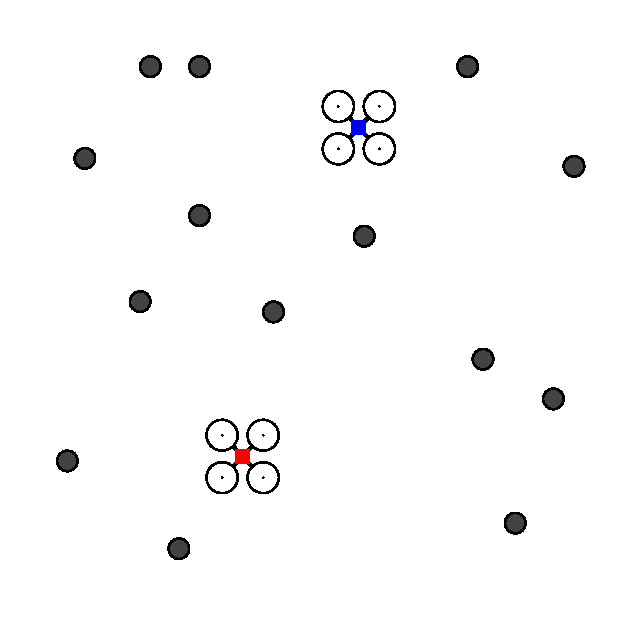
\includegraphics[width=0.3\textwidth]{./fig/photos/pip1.eps}

    \label{fig:pip1}
  }
  \subfloat[\centering \textbf{waypoint generation} - weighing and filtering] {
    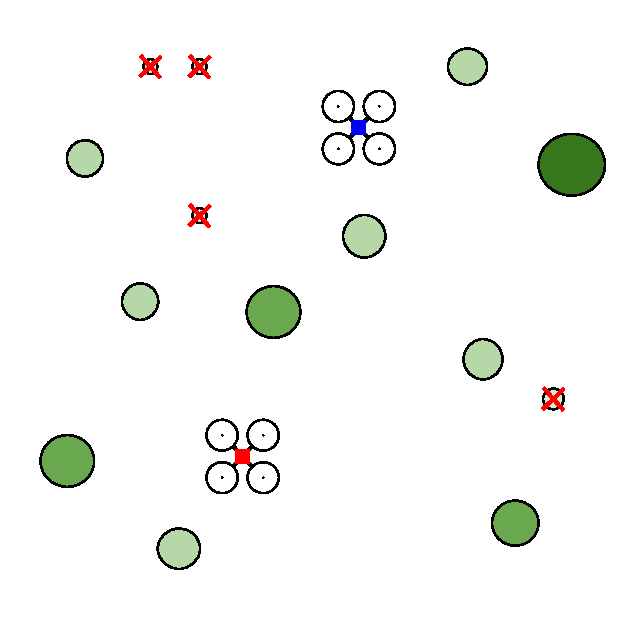
\includegraphics[width=0.3\textwidth]{./fig/photos/pip2.eps}
    \label{fig:pip2}
  }
  \subfloat[\centering \textbf{clustering} - assigning waypoints to \ac{UAV}s] {
    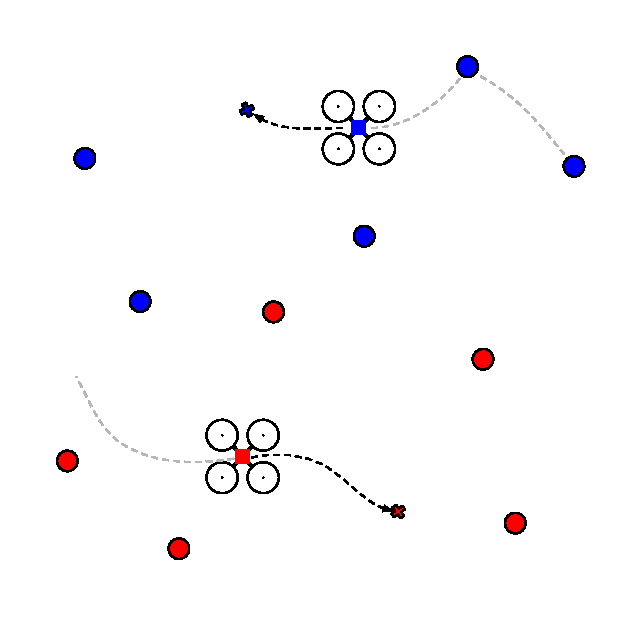
\includegraphics[width=0.3\textwidth]{./fig/photos/pip3.eps}
    \label{fig:pip3}
  }
  \newline
  \subfloat[\centering \textbf{waypoint filtering} - removal of recently visited waypoints based on short-term sensitivity] {
    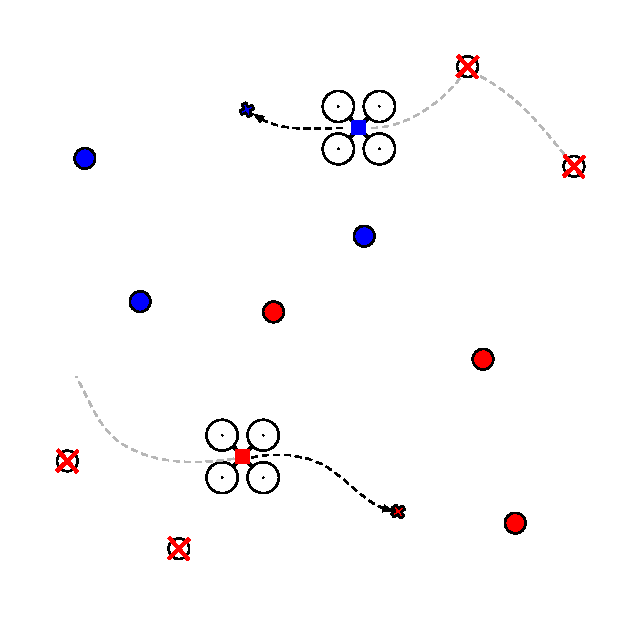
\includegraphics[width=0.3\textwidth]{./fig/photos/pip4.eps}
    \label{fig:pip4}
  }
  \subfloat[\centering \textbf{TSP} - optimal sequence determination] {
    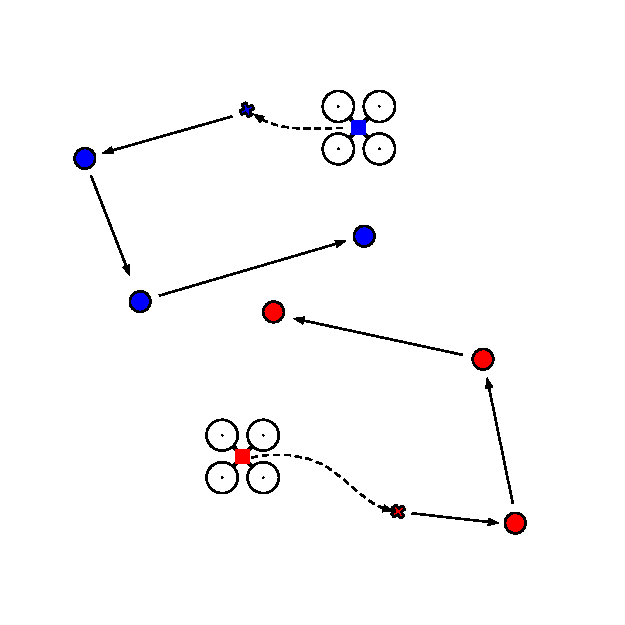
\includegraphics[width=0.3\textwidth]{./fig/photos/pip5.eps}
    \label{fig:pip5}
  }
  \subfloat[\centering \textbf{path planning} - find non-colliding paths connecting the waypoints] {
    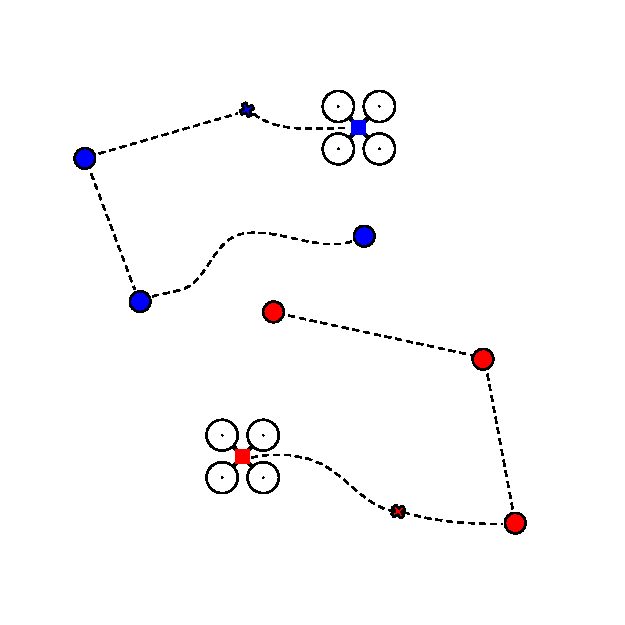
\includegraphics[width=0.3\textwidth]{./fig/photos/pip6.eps}
    \label{fig:pip6}
  }
  \caption{Individual steps of the system architecture.}
  \label{fig:pipeline}
\end{figure}% %%}

In the beginning, the exploitation waypoints are generated from the current \ac{MLEM} estimate (figure \ref{fig:pip1}).
Each waypoint is assigned a weight and only subset of waypoints with highest weights are processed to the next step (figure \ref{fig:pip2}).
The waypoints are assigned to the \ac{UAV}s using clustering method (figure \ref{fig:pip3}).
The recently visited exploitation waypoints are removed in the next step (figure \ref{fig:pip4}).
All points are connected into an optimal sequence (starting at the future position of the drone) using TSP (figure \ref{fig:pip5}).
Finally, non-colliding paths are planned for all \ac{UAV}s (figure \ref{fig:pip6}).
The more detailed description of each individual step follows in the next sections.


\mycomment{% %%{
  \section{multirobot approach}
  The previous chapter presented the method for localizing sources of ionizing radiation.
  %Given the collected measurements, it can compute the maximum likelihood estimate of the sources locations.
  Moreover, the sensitivity computed in the \ac{MLEM} method provides information about how much has been the area explored by the compton cameras onboard the \ac{UAV}s.

  This motivates the search strategy described in this section:
  The movement of the \ac{UAV}s should be controlled in a way that they simultaneously perform the following tasks:
  \begin{itemize}
    \item \textbf{exploration} - explore the least explored maps in the area of interest and increase the chance that so far unobserved sources of radiation will be detected
    \item \textbf{exploitation} - fly where the radioactive sources are likely present (based on the current maximum likelihood estimate) to improve the accuracy of the estimate. 
  \end{itemize}

%The maximum likelihood approach requires collecting as many measurements as possible to make the estimate more accurate.
%At the same time, the drones should explore the unexplored area to increase chance that the estimation method won't miss any source of ionizing radiation.
%The task for the mutirobotic system can be summarized as follows:
%\begin{itemize}
%  \item \textbf{exploration} - explore the least explored maps in the area of interest
%  \item \textbf{exploitation} - acquire more measurements from areas, where the source of ionizing radiation is likely present
%\end{itemize}
}% %%}





%%%%%%%%%%%%%%%%%%%%%%%%%%%%%%%%%
%%%%% WAYPOINTS GENERATION %%%%%%
%%%%%%%%%%%%%%%%%%%%%%%%%%%%%%%%%


\section{Waypoints generation}% %%{
\subsection{Exploitation}
\subsubsection{Local maxima filter}
The current estimate of ionizing radiation sources positions serves as an input for the waypoint generation method.
The map estimated by the \ac{MLEM} method is processed and local maxima of the map are detected.
Local maximum is a cell in the discretized map that has the highest value among all cells in its neighborhood. 
The size of the sliding window determining the neighborhood of each cell is a parameter that can be set.
The local maxima filter is illustrated in figure \ref{fig:filter}.

%figure filter%%{
\begin{figure}[!htb]
  \centering
  \subfloat[\centering input of the filter] {
    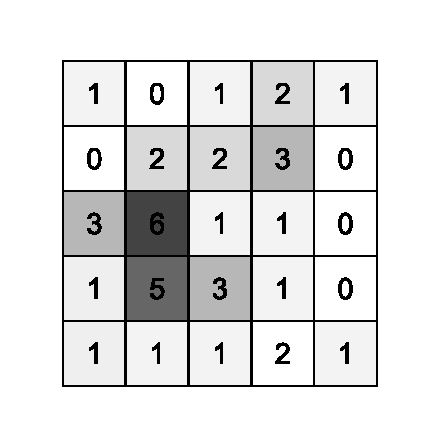
\includegraphics[width=0.2\textwidth]{./fig/photos/filter1.eps}

    \label{fig:fil1}
  }
  \subfloat[\centering filter window size 3] {
    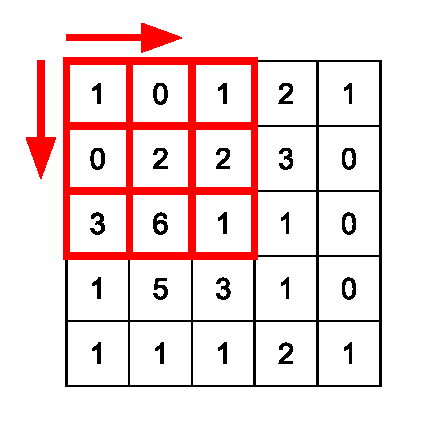
\includegraphics[width=0.2\textwidth]{./fig/photos/filter3.eps}
    \label{fig:fil2}
  }
  \subfloat[\centering detected local maxima] {
    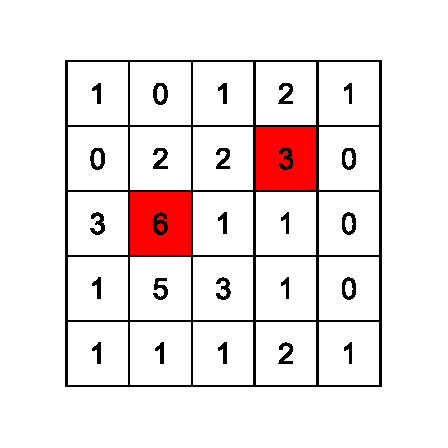
\includegraphics[width=0.2\textwidth]{./fig/photos/filter2.eps}
    \label{fig:fil3}
  }
  \caption{Local maxima filter demonstration}
  \label{fig:filter}
\end{figure}% %%}

\subsubsection{Waypoint weighting and filtration}
The waypoints associated with local maxima are weighted using following formula:
\begin{equation}
  w_{j_{weight}} = \frac{\lambda_{j}}{    s_{j_{normalized}} },
\end{equation}
where $s_{j_{normalized}} = \frac{ s_{j} }{ \underset{j}{\mathrm{max}}(s_{j})}$ is a sensitivity value normalized to range $[0, 1]$.
The purpose of the weighting step is following: it should prioritize the waypoints (local maxima) that are less explored (the sensitivity value is small compared to other waypoints).
The list of possible waypoints is then sorted from the highest $w_{j_{weight}}$ to the lowest.
Top $n$ waypoints based on the $w_{j_{weight}}$ are propagated further in the algorithm, the rest is ignored (parameter $n$ is set to $n = 10d$, where $d$ is number of drones used for exploitation).
The aim of filtering step is to remove the local maxima that were caused by noise in the \ac{MLEM} estimation.% %%}

\subsection{Exploration}
The task is to explore the map positions that have low sensitivity values (the probability that particle emitted from such position to be detected is low).
The process of generating waypoints for exploration is illustrated in figure \ref{fig:downsampling}.
The sensitivity vector $\mathbf{S}$ is downsampled by a mean filter with the stride equal to the filter window size.
The positions in the downsampled map are then sorted based on the mean sensitivity value.
Arbitrary percentage $p$ of the map poses with lowest sensitivity values is taken and exploration waypoints are generated in the centers of such downsampled map positions, as shown in figure \ref{fig:down3} for $p = 25\%$.

%figure downsampling%%{
\begin{figure}[!htb]
  \centering
  \subfloat[\centering input vector $\mathbf{S}$ in 2D] {
    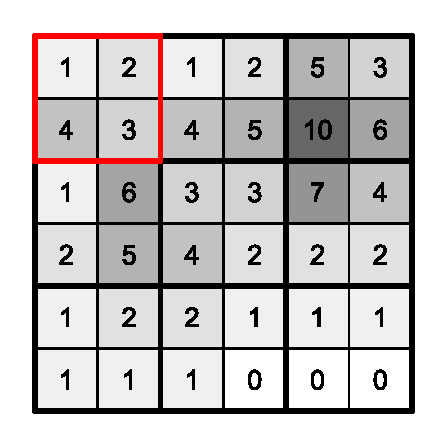
\includegraphics[width=0.25\textwidth]{./fig/photos/downsampling1.eps}

    \label{fig:down1}
  }
  \subfloat[\centering downsampled map (for window size and stride both equal 2)] {
    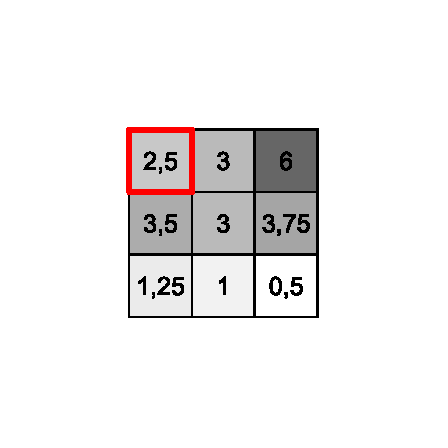
\includegraphics[width=0.25\textwidth]{./fig/photos/downsampling2.eps}
    \label{fig:down2}
  }
  \subfloat[\centering generated waypoints in the downsampled map for $p = 25\%$] {
    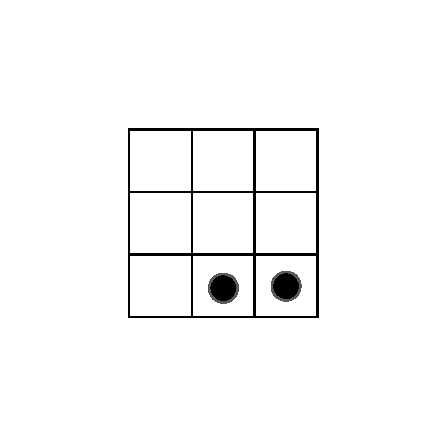
\includegraphics[width=0.25\textwidth]{./fig/photos/downsampling3.eps}
    \label{fig:down3}
  }
  \caption{Downsampling and waypoint generation process for exploration}
  \label{fig:downsampling}
\end{figure}% %%}


%%%%%%%%%%%%%%%%%%%%%%%
%%%%% CLUSTERING %%%%%%
%%%%%%%%%%%%%%%%%%%%%%%
\section{Clustering}% %%{
Clustering belongs to the group of unsupervised machine learning methods.
The goal of clustering is to partition the data into distinct groups (clusters), where data points within the same cluster are more similar to each other than to those in other clusters.
The euclidean distance is the measure of similarity used in this scenario.
The clustering algorithm of choice for the given task is \textbf{KMeans}, originally described in \cite{kmeans}.
The generated and filtered waypoints need to be assigned to the individual \ac{UAV}s. 
First step for that is clustering into groups, one group for each \ac{UAV} contributing to exploitation.

\subsection{KMeans algorithm}
The basic euclidean version of KMeans is defined as follows:
Let's denote data points to be clustered as $\{\mathbf{w}_{1}, \mathbf{w}_{2}, \dots , \mathbf{w}_{n}\}$.
The task is to assign each of the data points into one of the $k$ clusters, $\{C_{1}, C_{2}, \dots, C_{k}\}$.
Each cluster is represented by its centroid, $\mathbf{c}_{1}, \mathbf{c}_{2}, \dots, \mathbf{c}_{k}$.
The criterion function that should be minimized is then formulated as
\begin{equation}
  J = \sum_{i = 1}^{k} \sum_{\mathbf{w} \in C_{i}} \| \mathbf{w} - \mathbf{c}_{i} \|^{2}.
\end{equation}
In other words, we want to find such clusters so that the sum of distances between data points and corresponding centroids of clusters will be minimal.
\textbf{KMeans} is an iterative algorithm.
In each iteration, it assigns each data point to the nearest centroid based on the euclidean distance. 
After all data points are assigned to clusters, the centroids are updated by calculating the mean of all data points in each cluster. 
These two steps are repeated until convergence.
It is important to note that the outcome of the algorithm depends on the initialization of centroids and the method converge to local minima based on that initialization.

\subsection{Constrained KMeans and initialization}
For the purpose of assigning waypoints to the \ac{UAV}s, the optimality of the solution is not required.
However, we would like to assign waypoints to the \ac{UAV} that are in its neighborhood.
Moreover, we would like to guarantee that each \ac{UAV} has at least one point assigned (the standard version of KMeans does not guarantee non-emptiness of the clusters).
Therefore the constrained variant of KMeans \cite{constrained_kmeans} is used already implemented in \verb|k-means-constrained|\footnote{Available at: https://pypi.org/project/k-means-constrained/} python package.
The centroids are initialized at the future positions of the \ac{UAV}s.
The minimum number of waypoints in each cluster is set to $2$ (if the number of waypoints is large enough).% %%}

%%%%%%%%%%%%%%%%%%%%%%%
%%% FILTERING RECENT %%%
%%%%%%%%%%%%%%%%%%%%%%%
\section{Filtering recently visited waypoints}% %%{
The following assumption is made:
to acquire more measurements from different sides and localize the sources more precisely, it is better to keep the \ac{UAV}s in motion rather then statically hover at certain position for longer time.
No waypoint should be left unexplored for longer time.
Therefore are prioritized the waypoints that were not recently explored by any of the \ac{UAV}s (meaning that no \ac{UAV} was in a close proximity of the sensor in past seconds).
For that purpose, we define short-term sensitivity vector $\mathbf{\hat{S}}$, which is independent of the sensitivity vector $\mathbf{S}$ defined in equation \ref{eq:sen_iter}, 
although it is computed analogically.

Same as before, the matrix $\mathbf{\hat{S}}^{[n = 0]}$ is initialized with zeros.
Lets denote $V^{[n:n+1]}$ the set of viewpoints that were newly sampled after update step $n$ and needs to be processed. 
The short-term sensitivity matrix $\mathbf{\hat{S}}^{[n+1]}$ with elements $\hat{s}_{j}^{[n+1]}$ is computed as:
\begin{equation}
  \hat{s}_{j}^{[n+1]} = \alpha \hat{s}_{j}^{[n]} + \sum_{v \in V^{[n:n+1]}} s_{jv} \Delta_{v}. 
  \label{eq:sen_iter_shortterm}
\end{equation}
We may notice that the only difference between short-term sensitivity equation \ref{eq:sen_iter_shortterm} and sensitivity equation \ref{eq:sen_iter} is the scaling parameter $\alpha \in [0, 1)$.
The forgetting factor $\alpha$ scales past $\hat{s}_{j}$ values with some non-negative $<1$ number, making newly sampled and processed viewpoints more important.
The $\alpha$ is a custom parameter to be set, the default value is $\alpha = 0.95$ (assuming the short-term sensitivity is updated every $2$ seconds).% %%}

The filtering proceeds as follows:
\begin{equation}
  W_{filtered} = \{w_{x} | \hat{s}_{x} \ge \underset{w_{y} \in W}{\mathrm{median}}(\hat{s}_{y})\},
\end{equation}
where $W$ is the set of waypoints in the given cluster, $w_{x}$ are waypoints with short-term sensitivity $\hat{s}$ higher or equal to median of short-term sensitivity of all waypoints in the cluster.
Simply speaking, the half of the waypoints in the cluster that has been recently visited is removed in this step.
%%%%%%%%%%%%%%%%%%%%%%%
%%% TASK ASSIGNMENT %%%
%%%%%%%%%%%%%%%%%%%%%%%
\section{Sequence generation using TSP}% %%{

After assigning all waypoints into clusters, the optimal sequence of waypoints inside the cluster should be determined.
The proposed method is based on \ac{TSP}.
\subsection{Travelling salesman problem}
The \ac{TSP} is a classical problem in computer science. 
The problem can be formulated as follows: 
A complete oriented graph is given, where $V$ (set of vertices) represent locations that should be visited and $E$ (set of edges) represents the distances between then vertices.
The task is to find the path through the vertices (find a Hamiltonian cycle), so that each vertex is visited exactly once, the starting and ending point are the same and the distance of the path (the sum of weights assigned to the edges involved in the path) is minimal.
The edges of the graph are typically stored in a distance matrix $\mathbf{D}\in \mathbb{R}^{\left|V\right|\times\left|V\right|}$, where $d_{ab} \in \mathbf{D}$ represents the distance from vertex $a$ to vertex $b$.

\subsection{Problem modifications}
The problem of finding the optimal sequence of waypoints $\{v_{1}, v_{2}, \dots , v_{n}\}$ for an \ac{UAV} is transformed to the travelling salesman problem and solved using LKH solver\footnote{available at: http://webhotel4.ruc.dk/~keld/research/LKH/}.
However, we require some additional features, not only finding the minimal Hamiltonian cycle in the graph with respect to the euclidean distances between waypoints.
The starting vertex of the sequence should be the future position of the drone, let's denote it as vertex $v_{0}$.
Secondly, the path of the \ac{UAV} should not end in the starting vertex $v_{0}$, the last point of the sequence can be any of the waypoints $\{v_{1}, v_{2}, \dots, v_{n}\}$.
Because of that, we introduce dummy vertex denoted as $v_{F}$.
We formulate the transformed problem as follows.
The set of vertices of the graph is $\{v_{0}, v_{1}, v_{2}, \dots,v_{n}, v_{F}\} \in V$, where: 
\begin{itemize}
  \item $v_{0}$ is the starting point of the optimal sequence of waypoints
  \item $v_{1}, v_{2}, \dots, v_{n}$ are the points to be visited by the \ac{UAV} and   
  \item $v_{F}$ is the dummy vertex that serves as the last point of any sequence found by the solver.
\end{itemize}

The distance matrix $\mathbf{D}$ of euclidean distances between each pair of $\{v_{0}, v_{1}, v_{2}, \dots,v_{n},  v_{F}\}$ 

\begin{equation}
  \mathbf{D}_{eukl} = 
  \begin{pmatrix}
    0 & d_{0,1} & d_{0,2} & \dots & d_{0, n} & d_{1, F} \\
    d_{1,0} & 0 & d_{1,2} & \dots & d_{1, n} & d_{2, F} \\
    d_{2,0} & d_{2,1} & 0       & \dots & d_{2, n} & d_{3, F} \\
    \dots&\dots & \dots & \dots & \dots & \dots \\
    d_{n,0}& d_{n, 1} & d_{n, 2} & \dots & 0 & d_{n, F} \\
    d_{F, 0} & d_{F,1} & d_{F,2} & \dots & d_{F, n} & 0 
\end{pmatrix}
\end{equation}
is then modified in the following way:
a positive constant $M$ is introduced (it holds that $M>10\mathrm{max}(d),  \forall d \in \mathbf{D}_{eukl}$).
The purpose of this constant is to forbid some edges in the graph so that they couldn't be chosen by the numerical solver.
We set to $M$ all edges that connects the dummy vertex $v_{F}$ with all vertices $\{v_{1},v_{2}, \dots, v_{n}\}$, because we require the vertex $v_{F}$ to be the last one in the optimal sequence.
Additionally, the edge weight connecting the starting point $v_{0}$ and $v_{F}$ is also set to $M$.
Furthermore, the distance from any vertex $\{v_{1}, v_{2}, \dots, v_{n}\}$ to $v_{F}$ is set to $v_{0}$, same as the vertex from $v_{F}$ to $v_{0}$. 
The resulting modified distance matrix is

\begin{equation}
  \mathbf{D_{mod}} = 
  \begin{pmatrix}
    0 & d_{0,1} & d_{0,2} & \dots & d_{0, n} & M \\
    M & 0 & d_{1,2} & \dots & d_{1, n} & 0 \\
    M & d_{2,1} & 0       & \dots & d_{2, n} & 0 \\
    \dots&\dots & \dots & \dots & \dots & \dots \\
    M & d_{n, 1} & d_{n, 2} & \dots & 0 & 0 \\
    0 & M & M & \dots & M & 0 .  
\end{pmatrix}
\end{equation}

The picture \ref{fig:tsp} illustrates the situation for 3 waypoints.
The weights of the edges are painted in color.
The back color represents the euklidean dstance between the point.
The blue color represent edges whose value is set to $0$.
The weights of red edges are set to $M$.

\begin{figure}[!h]
    \centering
    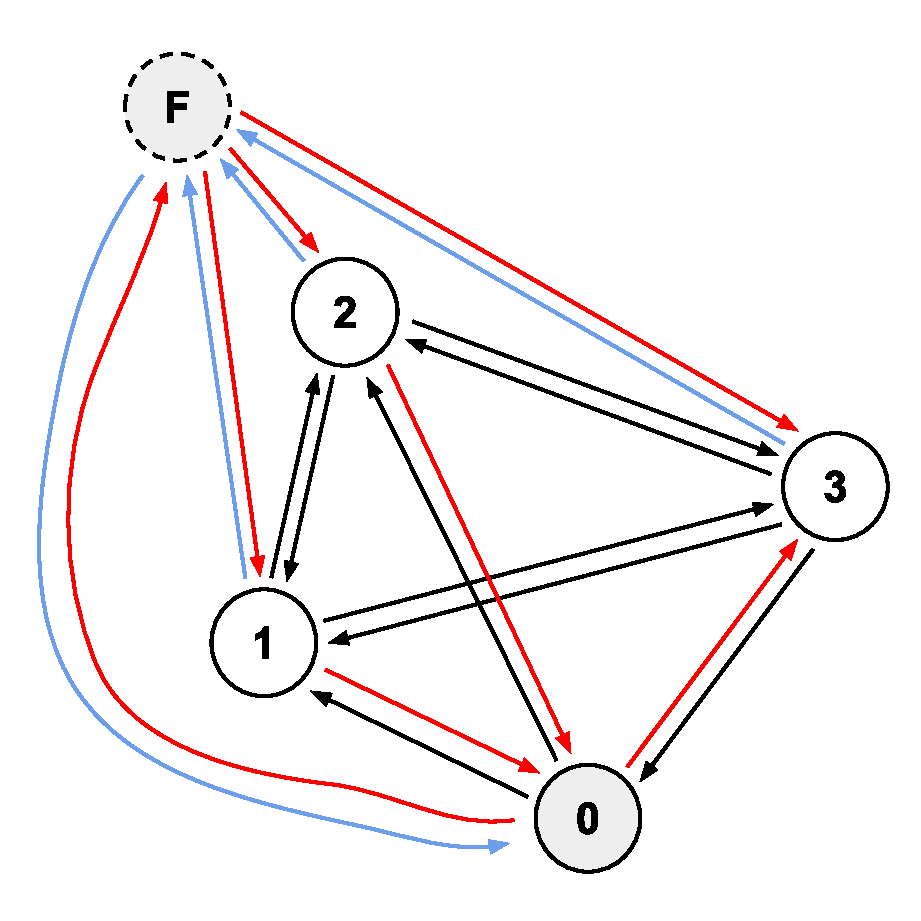
\includegraphics[width=0.4\textwidth]{./fig/photos/TSP.eps}
    \caption{An illustration of the modified distance matrix $\mathbf{D}_{mod}$ for the \ac{TSP} solver, that finds the optimal sequence of waypoints for each \ac{UAV}. 
    The vertex $v_{0}$ is the starting point of the sequence, vertices $\{v_{1}, v_{2}, v_{3}\}$ represent the waypoints to be visited by the \ac{UAV}, $v_{F}$ is an additional dummy virtual vertex. 
    The black edges represent the euclidean distance between corresponding vertices, the value of red edges is set to positive constant $M$, the value of blue edges is set to $0$. }
    \label{fig:tsp}
\end{figure}
%The modified distance matrix $\mathbf{D}_{mod}$ is then passed to the numerical solver.%%}

%%%%%%%%%%%%%%%%%%%%%%%
%%%% PATH PLANNING %%%%
%%%%%%%%%%%%%%%%%%%%%%%
\section{Path planning}% %%{
Once the sequence of waypoints for each \ac{UAV} is determined, the last step is a path planning.
The paths should be collision-free, the minimal distance between each pair of \ac{UAV}s should be at least $\SI{4}\meter$).
The planning method is based on astar planner implemented in the mrs uav system \cite{mrs_system}.
Each \ac{UAV} is assigned a certain priority.
The planning method is described in algorithm \ref{alg:planning}.
The paths are planned sequentially for each drone based on its priority.
Once a path for a drone is generated, the inflated (by the safety distance radius $r = \SI{4}\meter$) points of the path are considered as obstacles for all drones with the lower priority.
If any of the waypoints is not reachable (for example some drone with higher priority planned path in close distance to it), the waypoint is skipped.
The path is then smoothed by the mrs uav system \cite{mrs_system} onboard the drone and executed by the drone's controller.







\begin{algorithm}[!h]
\caption{Multi-path planning}\label{alg:cap}
\begin{algorithmic}

\Function {plan\_paths}{$drones\_waypoints, drones\_poses$}
  \State $planned\_paths \gets \{\}$
  \For {$drone \in drones$} \Comment{iterate over drones based on priority}
    \State $obstacles \gets \{\}$
    \For {$path \in planned\_paths$}
      \State $obstacles \gets obstacles \cup \Call{inflate\_points}{path}$ %\Comment{mark positions around already planned paths as obstacles}
    \EndFor
    \State $path \gets \{\}$
    \State $segment\_start \gets drone\_pose$
    \For {$waypoint \in drone\_waypoints$}

      \If{ $waypoint \in obstacles$}
        \State \textbf{continue}
      \EndIf
      \State $path\_segment \gets \Call{astar\_planner}{start, waypoint, obstacles}$
      \State $segment\_start \gets waypoint$
      \State $path \gets path \cup path\_segment$
    \EndFor
    \State $planned\_paths \gets planned\_paths \cup path$
  \EndFor
  \State \Return $planned\_paths$
\EndFunction


\end{algorithmic}
  \label{alg:planning}
\end{algorithm}% %%}





\mycomment{% %%{
  \subsection{Waypoint generation}
  s a first step, the $\lambda$ matrix (containing the current estimate of sources position) is processed by a local maximum filter. 
  The maximum filter works by sliding a window of a specified size over the $\lambda$.
  The central position of the sliding window is highlighted as local maxima if it is greater than all other values in the sliding window.

  Each waypoint (local maxima) is assigned with a weight $w$.
  The weight is defined as follows:
  \begin{equation}
    w_{j} = \frac{\lambda_{j}}{s_{j_{normalised}}}
  \end{equation},
  where $s_{j_{normalised}} = \frac{s_{j}}{\max_{J}( s_{j})}$ is a sensitivity value for given position $s_{j}$ divided by.
  Such formulation of $w_{j}$ prioritise the points with the highest current estimate of ionizing radiation, that are less explored (have lower sensitivity).

  \begin{algorithm}
  \caption{Planning pipeline}\label{alg:cap}
  \begin{algorithmic}
    \State $POI \gets \Call{get\_points\_of\_interest}$
    \State $POI_{sorted} \gets \Call{filter\_points}{POI}$
    \State $POI_{exploration} \gets \Call{get\_unexplored\_area\_points}$
    
    \State $future\_poses \gets \Call{get\_future\_drone\_poses}$

    \State $W_{exploitation} \gets \Call{clustering}{future\_poses}$
    \State $W_{exploration} \gets \Call{clustering}{future\_poses}$
    
    \State
  \end{algorithmic}
  \end{algorithm}



}% %%}




%% --------------------------------------------------------------
%% |                How to write thesis in LaTeX                |
%% --------------------------------------------------------------


%!TEX root = ../main.tex

\chapter{Results\label{chap:results}}
This chapter demonstrates the functionality of the proposed method\footnote{Videos from the experiments are available here: \url{http://mrs.felk.cvut.cz/theses/werner2023thesis}} for the localization of sources of ionizing radiation and its individual components.
Unfortunately, it was not possible to test the proposed methods using real sources of ionizing radiation for organizational reasons, since the use of radioactive materials is strictly regulated and requires coordination with state authorities (National Institute for Nuclear, Chemical and Biological Protection) and manufacturer of the \ac{pix}.
%That results in the fact that most of recorded data from real world experiments cant be used because the drones simply did not come close enough to other sources and 
Another problem is the absence of methods for comparison, that would be a) available, b) capable of localization of multiple sources using the Compton camera measurements.
Therefore we use the back-projection reconstruction method (described in Chapter \ref{chap:mlem_theory}) as a baseline.
This chapter presents results of the Monte Carlo simulation (Section \ref{chap:mcr}), 
performance of the system on recorded real-world data (Section \ref{chap:exp1}), 
in simulation (Section \ref{chap:exp2}) and in real-world experiment with simulated data (Section \ref{chap:exp3}). 
%The directional sensitivity of the \ac{pix} sensor, modelled via Monte Carlo simulation, is presented in \autoref{chap:mcr}.
%The evaluation of the \ac{MLEM} estimation approach, carried out on previously gathered data from experiments with real radioactive sources, is shown in \autoref{chap:exp1}.
%The functionality of the whole system (estimation method together with the proposed search strategy) in simulation is presented in \autoref{chap:exp2}.
%Finally, the whole system was also tested on real hardware with simulated radioactive sources, as shown in \autoref{chap:exp3}.

\section{Monte Carlo simulation of the sensor's sensitivity\label{chap:mcr}}
The assessment of the directional sensitivity of the \ac{pix} sensor was carried out using the Monte Carlo simulation described in Chapter \ref{chap:methods_estimation}.
Each omnidirectional simulated source (located $\SI{1}{\meter}$ from the sensor) emitted $10^{10}$ $\SI{662}{\kilo\electronvolt}$ photons from each position.
Shortly speaking, the simulator recorded the number of photons that a) reached the sensor's surface (more precisely, the \ac{CdTe} block, where the ionizing particles interact with \ac{CdTe} material) and b) undergone the interactions (Compton scattering, photoelectric absorption) leading to the Compton cone detection.  
Results of the Monte Carlo simulations are shown in \autoref{fig:monte_clar}.
The corresponding geometry of the \ac{CdTe} block is shown in \autoref{fig:monte_axes}.

The \ac{pix} sensor's directional sensitivity is depicted in \autoref{fig:monte_finalll}.
It can be observed that the probability of a particle being detected as a Compton event is nearly the same from all directions (more precisely, it varies from $3.79 \times 10^{-8}$ to $5.15\times 10^{-8}$).
The probability of reaching the sensor's surface (given the solid angle of the sensor from different positions) is shown in \autoref{fig:monte_reaching}.
A particle emitted in front of the sensor (along the x-axis) is more likely to hit the \ac{CdTe} block than another one emitted from the side (y-axis and z-axis), where the visible surface of the \ac{CdTe} block is the smallest.
On the other hand, the probability of Compton scattering as well as photoelectric absorption (that together lead to the detection of a Compton cone) depend on the trajectory of the incident and scattered photon.
The longer the intersection of an ionizing particle and the \ac{CdTe} block is, the more likely the interactions happen.
Therefore a photon reaching the sensor's surface from the side more likely causes the Compton measurement, as can be seen in \autoref{fig:monte_cone_from_hitting}.
In summary, both effects (probability of reaching the \ac{CdTe} block and probability of necessary interactions) neglect each other and lead to the almost uniform directional sensitivity of the \ac{pix} sensor.
%on the length of the intersection of the photon trajectory with the sensor \ac{CdTe} block.

The absolute values of estimated probabilities and also worth mentioning.
The \ac{pix} sensor with its dimensions $14.08 \times 14.08 \times 2 \ \si{\milli\meter}$ is very small compared to the distance between the \ac{UAV} carrying the sensor and sources of ionizing radiation.
Moreover, approximately only 1 of 100 $\SI{662}{\kilo\electronvolt}$ photons that reach the \ac{pix} sensor can be detected in the Compton camera mode.
For illustration: based on the simulation results, only $\approx 15$ Compton events can be possibly detected (on average) by a \ac{pix} sensor located $\SI{5}{\meter}$ 
from a source of $\SI{662}{\kilo\electronvolt}$ photons  with activity $\SI{1}{\giga\becquerel}$
(assuming exposure time $\SI{10}{\second}$). 
This estimate can be seen as an upper bound since it does not take into account other aspects of the detection process.
For example, other interactions might occur (the incident photon might be immediately absorbed without any Compton scattering), and the detection process might not estimate all the Compton cones correctly due to the noise caused by other particles detected by the Timepix detector at the same time.

% Answer: [trim={left bottom right top},clip]

\begin{figure}[!htb]% %%{
  \subfloat[$p(\mathrm{cone\ detected})$] {
    \centering
    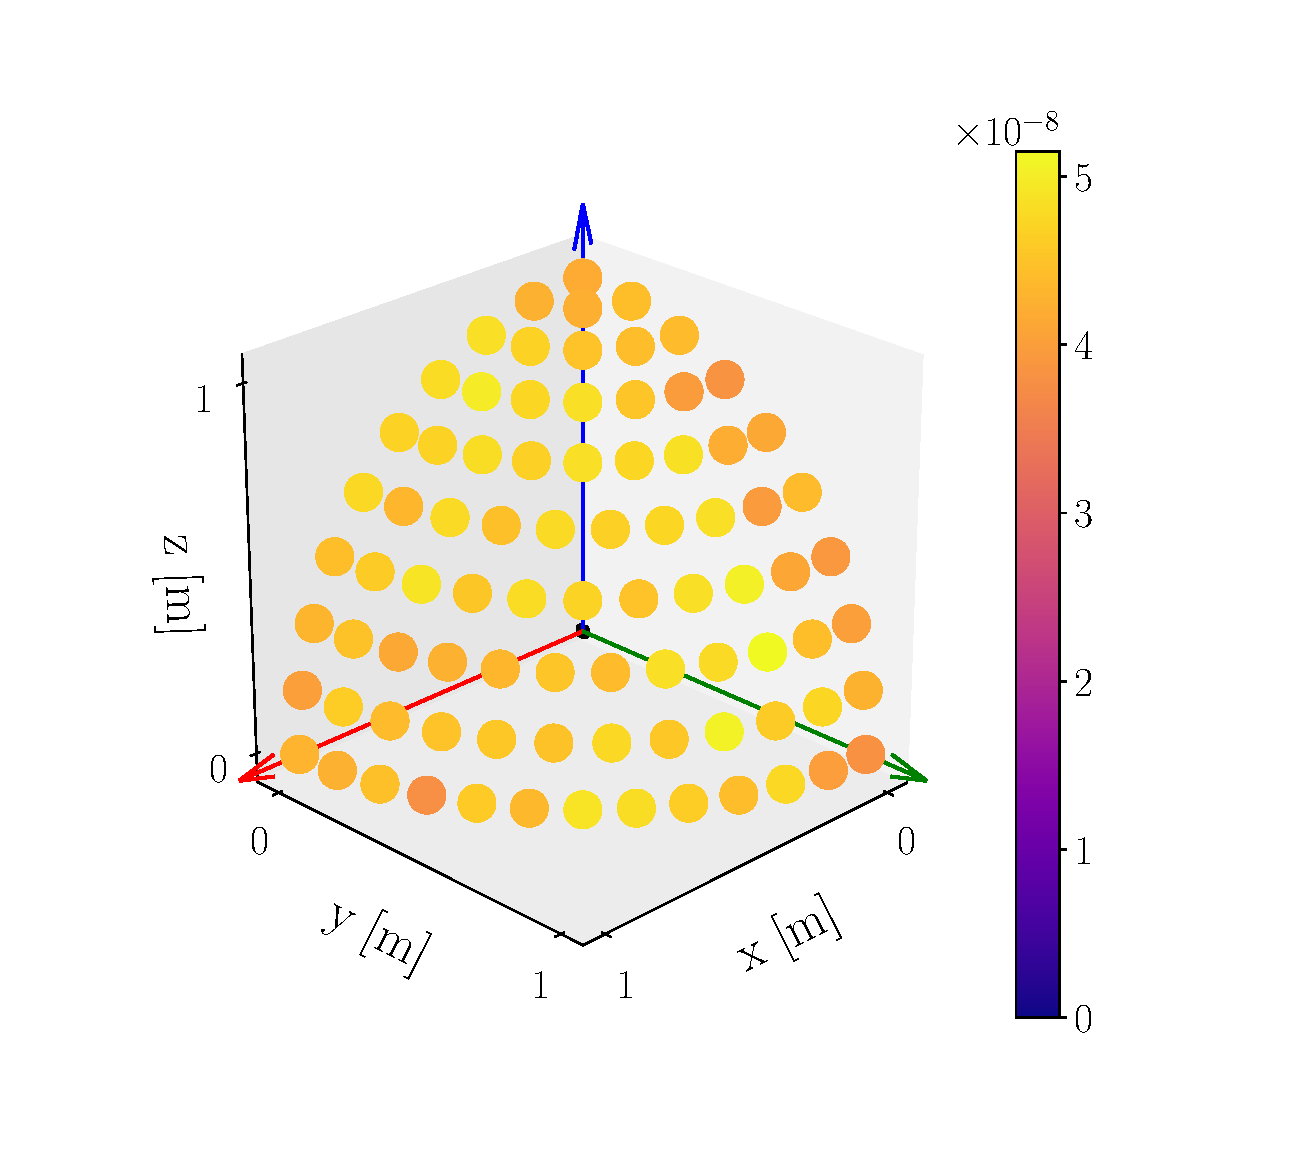
\includegraphics[width=0.42\textwidth,trim={1cm 1cm 2.5cm 1cm},clip]{./fig/photos/monte_carlo_final_prob.eps}
    \label{fig:monte_finalll}
  }
	\centering
  \subfloat[\ac{pix} sensor geometry. The \ac{CdTe} block (grey) has dimensions $14.08 \times 14.08 \times 2 \ \si{\milli\meter}$]{
    \centering
    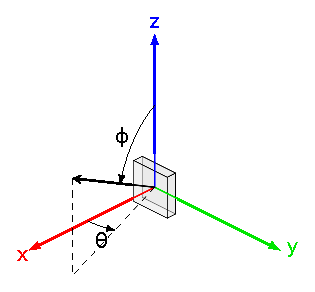
\includegraphics[width=0.4\textwidth]{./fig/photos/axes.eps}
    \label{fig:monte_axes}
  }
  \newline

  \noindent

  \subfloat[$p(\mathrm{reaching\ the\ sensor})$] {
    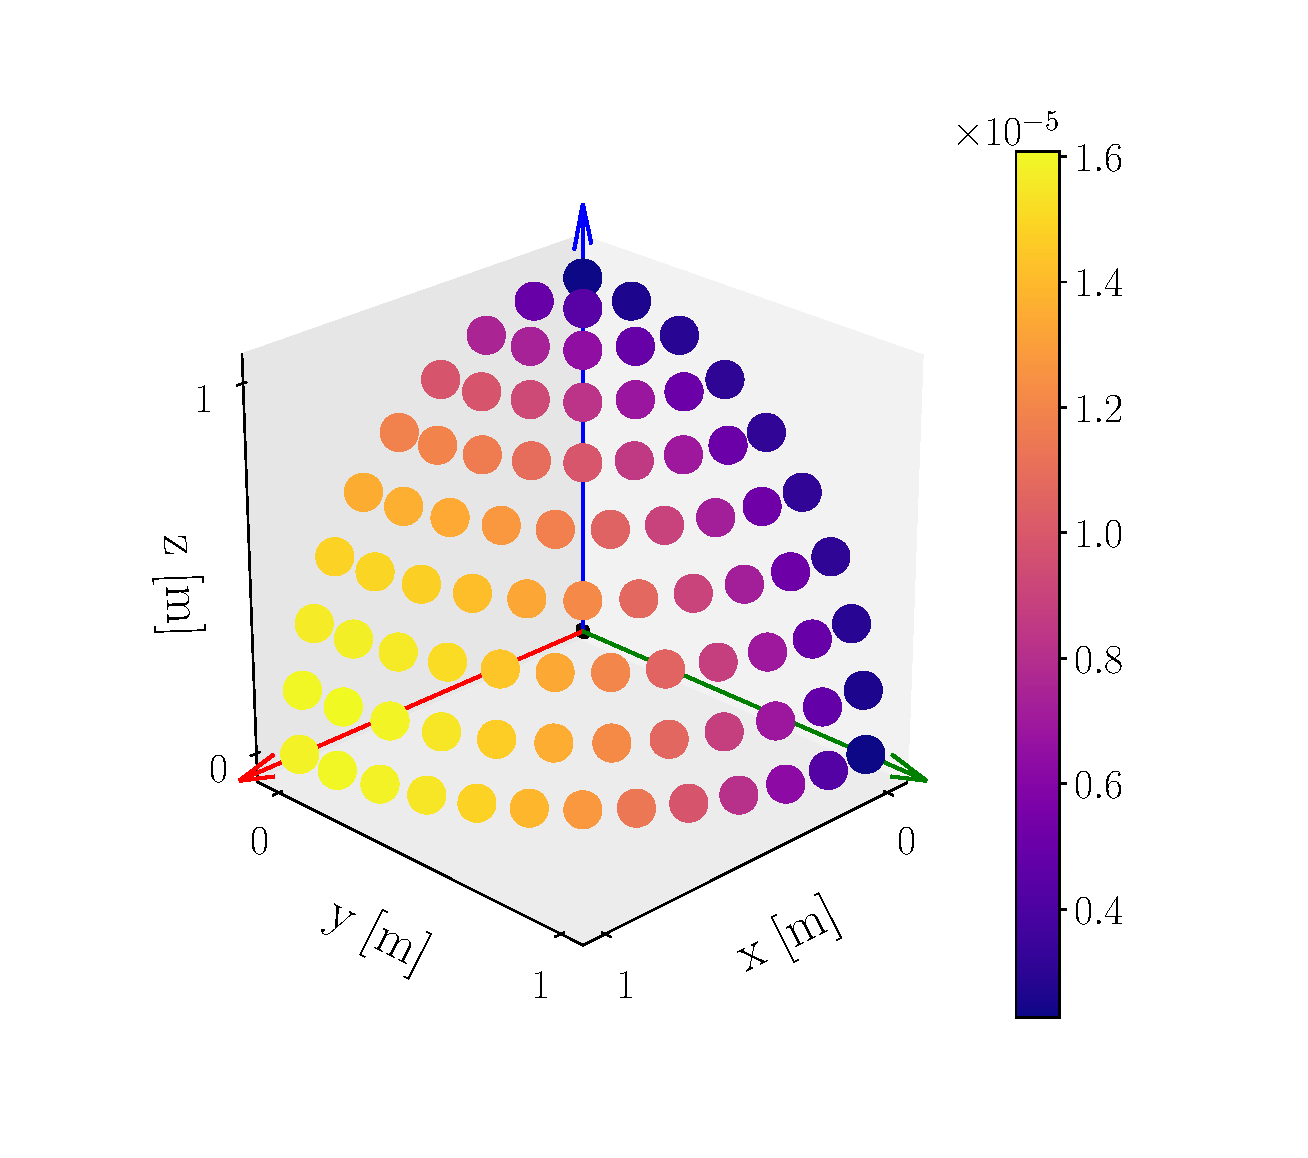
\includegraphics[width=0.42\textwidth,trim={1cm 1cm 1cm 1cm},clip]{./fig/photos/monte_carlo_total_activity.eps}
    \label{fig:monte_reaching}
  }
  \subfloat[$p(\mathrm{cone\ detected}\ |\ \mathrm{reaching\ the\ sensor})$] {
    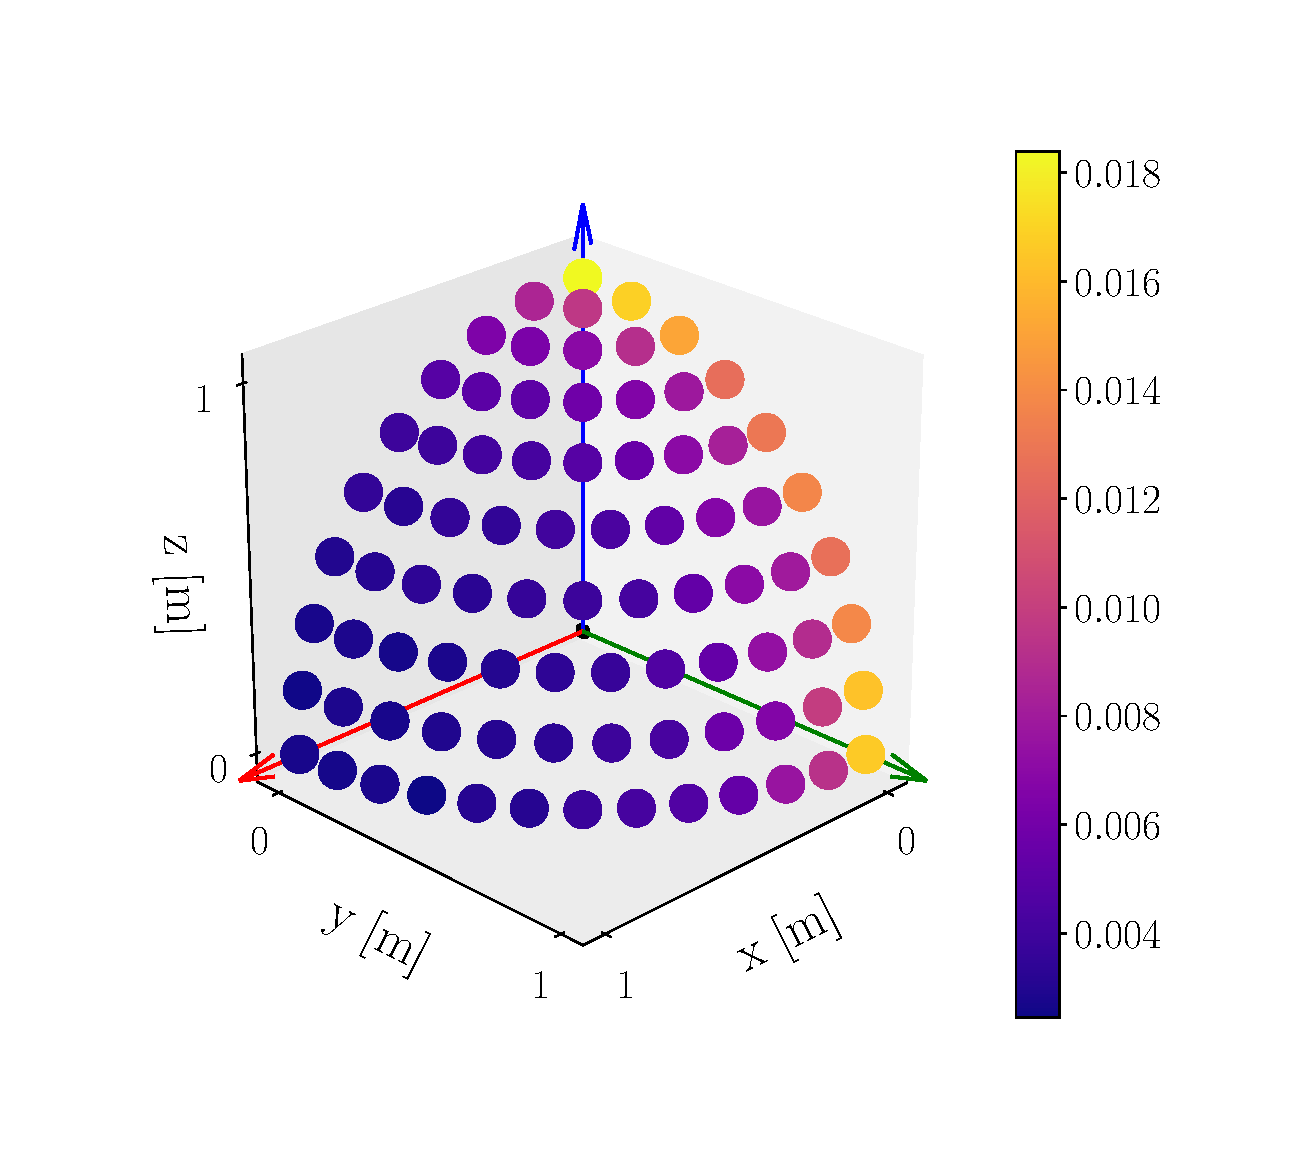
\includegraphics[width=0.42\textwidth,trim={1cm 1cm 1cm 1cm},clip]{./fig/photos/monte_carlo_fraction.eps}
    \label{fig:monte_cone_from_hitting}
  }
  \caption{Direction sensitivity of the \ac{pix} sensor (geometry of the sensor depicted in \protect\subref{fig:monte_axes}). 
  The probability that a $\SI{662}{\kilo\electronvolt}$ photon emitted at the corresponding position causes a Compton cone is depicted in \protect\subref{fig:monte_finalll}. 
  The probability that the particle emitted at a given position reaches the detector is depicted in \protect\subref{fig:monte_reaching}. 
  Lastly, the probability that a photon (that reached the sensor) causes a Compton cone is illustrated in \protect\subref{fig:monte_cone_from_hitting}.}
  \label{fig:monte_clar}
\end{figure}% %%}
%%%%%%%%%%%%%%%%%%%%%%%%%%%%%%%%%%%%%%%%%
\newpage
\section{Evaluation of MLEM method based on real-world data\label{chap:exp1}}
The proposed \ac{MLEM} method for radiation mapping has been tested using data from real-world experiments that were carried out in September 2022 (before the work on this thesis started).
Although the pre-recorded real-world data were collected in realistic conditions with real sensors and sources of ionizing radiation, the prerecorded data do not allow to fully test capabilities of the proposed system.
The reason is the strong dependency between drones trajectories during the experiment and recorded measurements (caused by properties of the ionizing radiation, such as the inverse square law, that is significantly reducing distance from which a radioactive source might be perceived). 
Therefore the outcome of reconstruction strongly depends on in which areas the drones flew during the recorded experiments.

\subsection{Setup and course of the experiment (data collection)}
The area of interest of size $\approx 40 \times 30\ \si{\meter}$ was scanned by a group of four \ac{UAV}s equipped with \ac{pix} sensor.
The \ac{UAV}s were localized using \ac{GPS}.
The drones were controlled by the method proposed in \cite{baca2021gamma}.
In the beginning of the experiment, the drones were following a predefined trajectory covering the whole area of interest uniformly.
After the first 8 Compton cones were detected, three drones were flying $\SI{3}{\meter}$ above the ground encircling the current single-hypothesis estimate of the source position (filtered by a \ac{LKF}). 
The last drone with flight height $\SI{6}{\meter}$ was following a predefined path covering the whole area.
Four sources of Cesium-137 with activity $1900, 500, 180, 50\ \si{\mega\becquerel}$ were located at positions shown in \autoref{e1:gt}.
During the run of the experiment, the drones were mostly encircling the $\SI{500}{\mega\becquerel}$ source position.
The fourth \ac{UAV} flying $\SI{6}{\meter}$ above the ground twice detected photons originating from the $\SI{1900}{\mega\becquerel}$ source. 
As a consequence, the single hypothesis moved towards the strongest source. However, the group of \ac{UAV}s moved back to the $\SI{500}{\mega\becquerel}$ source after a while.
The whole experiment took $\approx \SI{10}{\minute}$, and $263$ Compton cones were recorded.

\subsection{Evaluation of the MLEM method}
The results of the proposed \ac{MLEM} estimation method are presented in \autoref{fig:e1_all}.
The area of interest was discretized with $\SI{1}{\meter}$ resolution, and the number of iterations of the \ac{MLEM} method was set to 10.
The viewpoints (positions of the drones) were sampled with $\SI{5}{\hertz}$, and the \ac{MLEM} estimate was updated every $\SI{2}{\second}$.
The uncertainty of the cone angle  
The final estimate of the emission intensity $\bm{\lambda}$ (based on all data acquired during the experiment) is presented in \autoref{e1:lam}. 
The sensitivity of detection (\autoref{e1:sen}) confirms what was stated before - the drones were mostly encircling the $\SI{500}{\mega\becquerel}$ source at position $(-2, -10)$, which was also correctly localized.
The area in the vicinity of the $\SI{1900}{\mega\becquerel}$ source at position $(16, 0)$ was much less explored by the \ac{UAV}s (and therefore fewer Compton cones originating there were recorded).
Despite the much lower sensitivity in that area, the \ac{MLEM} method estimated some local maxima in the neighbourhood of the true position of the strongest source.
The two weakest sources of radiation are indistinguishable from the noise.



\mycomment{% %%{
  \subsection{Convergence of the MLEM algorithm}
The convergence of \ac{MLEM} algorithm (using \ac{MSE} as the metric) is shown in \autoref{e1:mse}. 
\ac{MSE} in this scenario is defined as
\begin{equation}
MSE = \frac{1}{J} \sum_{j = 0}^{J} (\lambda_{j_{normalized}} - g_{j})^{2},
\end{equation}
where the ground truth is defined as $g_{j} = \frac{\mathrm{source\ activity}}{\mathrm{max}(\mathrm{source\ activity})}$ at the sources locations and $g_{j} = 0$ elsewhere.
The iterative \ac{MLEM} algorithm is initialized with back-projection (\autoref{e1:bp}). 
We can see in \autoref{e1:mse} that the decrease of the $MSE$ stopped after a few iterations.

\begin{figure}
	\centering
    \includegraphics[width=0.5\textwidth,trim={0 0.5cm 2cm 1cm},clip]{./fig/photos/auto_mse_realworld.eps}
		\caption{\ac{MSE} of the \ac{MLEM} method applied to the pre-recorded data from real-world experiments.}
    \label{e1:mse}
\end{figure}
}% %%}



\begin{figure}[!htb]% %%{
  \centering
  \subfloat[estimate of ionizing radiation intensity $\bm{\lambda}$ (rescaled)] {
    \includegraphics[width=0.5\textwidth,trim={0 0.5cm 2cm 1cm},clip]{./fig/photos/auto_lam.eps}
    \label{e1:lam}
  }
  \subfloat[ground truth positions of sources ($\si{\mega\becquerel}$)] {
    \includegraphics[width=0.5\textwidth,trim={0 0.5cm 2cm 1cm},clip]{./fig/photos/auto_gt.eps}
    \label{e1:gt}
  }
  \newline
  \noindent 
  \subfloat[back-projection (number of Compton cones)] {
    \includegraphics[width=0.5\textwidth,trim={0 0.5cm 2cm 1cm},clip]{./fig/photos/auto_bp.eps}
    \label{e1:bp}
  }
  \subfloat[sensitivity of detection $\mathbf{s}$] {
    \includegraphics[width=0.5\textwidth,trim={0 0.5cm 2cm 1cm},clip]{./fig/photos/auto_sen.eps}
    \label{e1:sen}
  }
  \caption{The \ac{MLEM} method evaluated on pre-recorded real-world data.}
  \label{fig:e1_all}
\end{figure}% %%}
%%%%%%%%%%%%%%%%%%%%%%%%%%%
\subsection{Summary}
The results of the \ac{MLEM} reconstruction are heavily affected by a noise in measurements.
First of all, the \ac{UAV}s were localized using \ac{GPS} method that might be effected by a position error of several meters.
The position error propagates to the uncertainty of the Compton cone origins.
Furthermore, the real \ac{pix} sensors produced many outliers --- e.g. Compton cones pointing upwards or not intersecting any source position. 
The noisy measurements are probably caused by the working principle of an unshielded single-layer Compton camera, where ionizing particles coming from different directions might affect the Cone reconstruction procedure.
This might be a limiting factor for the localization of multiple sources of ionizing radiation (with high emission activity) that are close to each other.
The single-layer Compton camera is able to estimate the direction of incoming ionizing photons only if the number of interactions detected by the Timepix3 pixel detector inside the \ac{pix} sensor is relatively low and corresponding interactions can be paired together correctly.
However, the presence of multiple sources in close vicinity increases the particle flux and may potentially increase the number of outliers.

In summary, the comparison of \ac{MLEM} estimate (\autoref{e1:lam}) and back-projection (\autoref{e1:bp}) show that the \ac{MLEM} significantly improved the reconstruction quality.
The $\SI{1900}{\mega\becquerel}$ source was localized (despite the low number of recorded photons originating there) 
thanks to the weighting of the estimate with the sensitivity of detection in the \ac{MLEM} algorithm.
Better results might be achieved by using an active search strategy, where the drones are controlled in order to improve the quality of the current \ac{MLEM} estimate.









%%%%%%%%%%%%%%%%%%%%%%%%%%%%%%%%%%%%%%%%%%%%%%%%%%%%%%%%
%%%%%%%%%%%%%%%%%%%%%%%%%%%%%%%%%%%%%%%%%%%%%%%%%%%%%%%%%%%%%%%%%%%%%
%%%%%%%%%%%%%%%%%%%%%%%%%%%%%%%%%%%%%%%%%%%%%%%%%%%%%%%%%%%%%%

\section{Evaluation of MLEM and search strategy in simulation\label{chap:exp2}}
The \ac{MLEM} estimation method has been tested together with the proposed search strategy in \textit{Gazebo} simulator. 
The results were compared with the back-projection method, that served as a baseline.

\begin{figure}[!htb]
  \centering
    \includegraphics[width=0.9\textwidth]{./fig/photos/simu_search.png}
  \caption{Experiments in \textit{Gazebo} simulator. The \ac{UAV}s are autonomously mapping sources of ionizing radiation place in the area $40 \times 40\ \si{\meter}$ (resolution $r = \SI{1}{\meter}$). 
  The current \ac{MLEM} estimate is visualized using blue-red-green distribution and black numbers denoting the relative activity of local maxima at the given position. 
  The drones follow the trajectories (red arrows) to visit waypoints (depicted as transparent spheres). Two drones are designated for exploitation (red and green waypoints) and one for exploration (blue waypoints).}
  \label{fig:simu_search}
\end{figure}
\subsection{Simulated experiment 1}
%\subsubsection{Experiment setup}
The distribution and activity of the radioactive sources were the same as in the real-world experiments described in the previous section.
Three drones flying $\SI{3}{\meter}$ above the ground were used during the experiment.  
The simulation process (visualized in \textit{RViz}) is shown in \autoref{fig:simu_search}.
Two drones were designated for exploitation (visiting the positions where the sources of radiation are present based on the latest \ac{MLEM} estimate), and one for exploration (visiting positions with the lowest sensitivity). 
The drones were initialized at positions ($-15, -10$), ($-5, -10$) and ($5, -10$) and controlled by the proposed search strategy in the rest of the experiment.
\subsubsection{Measurement noise}
Extra noise was added to the measurements to model the real-world conditions.
The inaccuracy in the drone position (resulting in the shifted origin of the Compton cone) was modelled with the Normal distribution $\mathcal{N}(\mu_{pos}, \sigma_{pos})$ with zero means $\mu_{pos} = 0$ and standard deviation $\sigma_{pos} = \SI{1.5}{\meter}$. 
The noise in energy measurements of the simulated \ac{pix} sensor was modeled the Normal distribution $\mathcal{N}(\mu_{energy}, \sigma_{energy})$ with zero mean $\mu_{energy} = 0$ and standard deviation $\sigma_{energy} = \SI{7}{\kilo\electronvolt}$.

\subsubsection{Results}
The results of the \ac{MLEM} reconstruction are presented in \autoref{fig:e2}.
The progress of radiation mapping is illustrated in \autoref{e2:lam1} (time $t = \SI{25}{\second}$) and \autoref{e2:lam2} ($t = \SI{100}{\second}$), corresponding sensitivity of detection is presented in \autoref{e2:sen1}, \autoref{e2:sen2}.
The active search strategy controlled the drones in order to acquire more measurements, which significantly improved the initial inaccurate estimate (based on a smaller number of Compton cones).
We may notice that after $\SI{100}{\second}$ of flight the \ac{UAV}s correctly localized the $\SI{1900}{\mega\becquerel}$ , $\SI{500}{\mega\becquerel}$ and $\SI{280}{\mega\becquerel}$ sources of simulated ionizing radiation.
The $\SI{50}{\mega\becquerel}$ source was not recognized due to its low emission activity or because it was filtered out during the later iterations of the \ac{MLEM} algorithm.
The \ac{MLEM} method significantly improved the solution compared to the back-projection illustrated in \autoref{e2:bp}.

\subsubsection{Summary}
Three sources with the highest emission activity were correctly localized in less than $\SI{100}{\second}$.
The proposed \ac{MLEM} estimation method, together with the autonomous search strategy, worked as intended.
Although the \ac{MLEM} method does not estimate the positions of sources perfectly for a small number of measurements, the active search strategy guides the \ac{UAV}s in order to acquire more measurements, which further improves the estimate's quality.
The extensive testing in simulations showed that the inaccuracy in the Compton cones' origins significantly reduces the quality of reconstruction, which highlights the need for accurate localization of drones during real-world experiments.
In summary, the experiment showed that the proposed method is capable of autonomous localization of multiple sources of ionizing radiation (of different emission activity).




\subsubsection{Simulation vs. reality}
The simulated noise in the drone's position and energies helped to bring the simulation closer to real-world conditions.
However, the used simulator of ionizing radiation simulates each source-sensor pair independently, which ignores the fact that ionizing particles from multiple sources might interact in the sensor at the same time (causing outliers), therefore the simulation is not as accurate as it could be.
Improving the simulator in order to process interactions caused by different sources simultaneously presents a possible direction for future research.

\begin{figure}[!htb]% %%{
  \centering
  \subfloat[($t = \SI{25}{\second}$) source intensities $\bm{\lambda}$ (rescaled) ] {
    \includegraphics[width=0.5\textwidth,trim={0 0.5cm 2cm 1cm},clip]{./fig/photos/auto_simulation_lam_1.eps}
    \label{e2:lam1}
  }
  \subfloat[($t = \SI{25}{\second}$) sensitivity of detection $\mathbf{s}$ ] {
    \includegraphics[width=0.5\textwidth,trim={0 0.5cm 2cm 1cm},clip]{./fig/photos/auto_simulation_sen_1.eps}
    \label{e2:sen1}
  }
  \newline
  \noindent
  \subfloat[($t = \SI{100}{\second}$) source intensities $\bm{\lambda}$ (rescaled) ] {
    \includegraphics[width=0.5\textwidth,trim={0 0.5cm 2cm 1cm},clip]{./fig/photos/auto_simulation_lam_2.eps}
    \label{e2:lam2}
  }
  \subfloat[($t = \SI{100}{\second}$) sensitivity of detection $\mathbf{s}$ ] {
    \includegraphics[width=0.5\textwidth,trim={0 0.5cm 2cm 1cm},clip]{./fig/photos/auto_simulation_sen_2.eps}
    \label{e2:sen2}
  }
  \newline
  \noindent
  \subfloat[($t = \SI{100}{\second}$) back projection (number of cones)] {
    \includegraphics[width=0.5\textwidth,trim={0 0.5cm 2cm 1cm},clip]{./fig/photos/auto_simulation_bp.eps}
    \label{e2:bp}
  }
  \subfloat[ground truth positions of sources ($\si{\mega\becquerel}$)] {
    \includegraphics[width=0.5\textwidth,trim={0 0.5cm 2cm 1cm},clip]{./fig/photos/auto_simulation_gt.eps}
    \label{e2:gt}
  }
  \caption{Results of the experiment with three \ac{UAV}s and four sources of ionizing radiation simulated in \textit{Gazebo}. 
  The progress of the \ac{MLEM} reconstruction method is shown in \protect\subref{e2:lam1}, \protect\subref{e2:sen1} and \protect\subref{e2:lam2}, \protect\subref{e2:sen2}.
  %The output of the \ac{MLEM} method after $\SI{25}{\second}$ (\autoref{e2:lam1}, \autoref{e1:sen1}) and after $\SI{100}{\second}$ (\autoref{e2:lam2}, \autoref{e1:sen2}) is presented. 
  %We can see that the quality of the \ac{MLEM} estimate improved during the flight thanks to the active search strategy.
  The back-projection of all cones measured in the first $\SI{100}{\second}$ is shown in \protect\subref{e2:bp}.  }
  \label{fig:e2}
\end{figure}% %%}


\mycomment{
\begin{figure}[!htb]% %%{
  \centering
  \subfloat[($t = \SI{25}{\second}$) source intensities $\bm{\lambda}$ (rescaled) ] {
    \includegraphics[width=0.5\textwidth,trim={0 0.5cm 2cm 1cm},clip]{./fig/photos/auto_simulation_lam_1.eps}
    \label{e2:lam1}
  }
  \subfloat[($t = \SI{25}{\second}$) sensitivity of detection $\mathbf{s}$ ] {
    \includegraphics[width=0.5\textwidth,trim={0 0.5cm 2cm 1cm},clip]{./fig/photos/auto_simulation_sen_1.eps}
    \label{e2:sen1}
  }
  \newline
  \noindent
  \subfloat[($t = \SI{100}{\second}$) source intensities $\bm{\lambda}$ (rescaled) ] {
    \includegraphics[width=0.5\textwidth,trim={0 0.5cm 2cm 1cm},clip]{./fig/photos/auto_simulation_lam_2.eps}
    \label{e2:lam2}
  }
  \subfloat[($t = \SI{100}{\second}$) sensitivity of detection $\mathbf{s}$ ] {
    \includegraphics[width=0.5\textwidth,trim={0 0.5cm 2cm 1cm},clip]{./fig/photos/auto_simulation_sen_2.eps}
    \label{e2:sen2}
  }
  \newline
  \noindent
  \subfloat[($t = \SI{100}{\second}$) back projection (number of cones)] {
    \includegraphics[width=0.5\textwidth,trim={0 0.5cm 2cm 1cm},clip]{./fig/photos/auto_simulation_lam.eps}
    \label{e2:bp}
  }
  \subfloat[ground truth positions of sources ($\si{\mega\becquerel}$)] {
    \includegraphics[width=0.5\textwidth,trim={0 0.5cm 2cm 1cm},clip]{./fig/photos/auto_simulation_sen.eps}
    \label{e2:gt}
  }
  \caption{Lorem ipsum}
  \label{fig:e2}
\end{figure}% %%}

}
\subsection{Simulated experiment 2}
The ability to map multiple sources of ionizing radiation is demonstrated on the following simulated scenario:
the size of the area, number of drones, simulated noise and other parameters remain the same as in the previous experiment.
Only the activity of sources is set to the same value for convenience.
The source is considered as detected if the estimated emission activity ($\bm{\lambda}$ rescaled to $0-1$ range) at the ground-truth source position exceeds detection threshold $0.5$ (in the vicinity of $\SI{2}{\meter}$ around the ground-truth position) and remains above threshold $0.3$ during the rest of the experiment.
Since the radiation emission is a stochastic process, the same instance was repeated multiple times.
Results are presented in \autoref{fig:eval}. % shows the detection times for multiple simulated sources if the same activity. 
\begin{figure}[!htb]
  \centering
  \subfloat[Four sources with activity $\SI{100}{\mega\becquerel}$] {
    \includegraphics[width=0.4\textwidth,trim={1cm 0 1.5cm 1.2cm},clip]{./fig/photos/auto_eval1.eps}
    \label{fig:eval1}
  }
  \subfloat [Four sources with activity $\SI{500}{\mega\becquerel}$]{
    \includegraphics[width=0.4\textwidth,trim={1cm 0 1.5cm 1.2cm},clip]{./fig/photos/auto_eval2.eps}
    \label{fig:eval2}
  }
  \newline\noindent
  \subfloat [Four sources with activity $\SI{2000}{\mega\becquerel}$]{
    \includegraphics[width=0.4\textwidth,trim={1cm 0 1.5cm 1.2cm},clip]{./fig/photos/auto_eval3.eps}
    \label{fig:eval3}
  }
  \subfloat [Ground truth positions]{
    \includegraphics[width=0.45\textwidth,,trim={0cm 0 1.5cm 1.2cm}, clip ]{./fig/photos/auto_eval_gt.eps}
    \label{fig:eval4}
  }
  \caption{The number of correctly detected sources with the same emission activity (located at positions \protect\subref{fig:eval4}). Dashed lines represent the individual experiments (each scenario was repeated $5$ times), the black line is the average. The detection was evaluated every $5$ seconds.}
  \label{fig:eval}
\end{figure}
\subsubsection{Results}
We can see that the low emission activity of the sources prolongs the detection time (\ref{fig:eval1}), however, the method was still able to localize positions of the $3$ sources (on average) in less than $\SI{250}{\second}$.
The method was able to correctly localize four $\SI{2000}{\mega\becquerel}$ sources is less than  $\SI{170}{\second}$ in all scenarios.
We may notice that the number of detected sources also sometimes decreased during the time (see the purple line in \ref{fig:eval3}). 
This shows that the method do not perfectly estimate the relative emission activity of the sources, which is caused by the stochastic nature of radioactive decay and limited number of measurements.



%%%%%%%%%%%%%%%%%%%%%%%%%%%%%%%%%%%%%%%%%%%%%%%%%%%%%%%%%%%%%%%%%%%%%%%
%%%%%%%%%%%%%%%%%%%%%%%%%%%%%%%%%%%%%%%%%%%%%%%%%%%%%%%%%%%%%%%%%%%%%%%%%%
%%%%%%%%%%%%%%%%%%%%%%%%%%%%%%%%%%%%%%%%%%%%%%%%%%%%%%%%%%%%%%%%%%%%%%


\section{Real-world experiment with simulated radiation\label{chap:exp3}}
The proposed search strategy has been tested using real \ac{UAV}s during the field experiments.
Since the real sources of radiation were not available, the ionizing radiation was simulated onboard each \ac{UAV}.
The main purpose of the experiment was to test the search strategy with real hardware and gain some experience with real-world conditions, where many things are not as simple as in simulation.
\begin{figure}[!htb]
  \centering
  \subfloat[The DJI f450 drones used during the experiments.] {
    \includegraphics[width=0.5\textwidth]{./fig/photos/experiments.jpg}
    \label{fig:d1}
  }
  \subfloat [The area of interest and \ac{UAV}s searching for the (simulated) sources of ionizing radiation.]{
    \includegraphics[width=0.5\textwidth]{./fig/photos/pole3.png}
    \label{fig:d2}
  }
  \caption{Field experiments with real hardware. The drones \protect\subref{fig:d1} were mapping the simulated radioactive sources located somewhere in the open field \protect\subref{fig:d2}.}
  \label{fig:field}
\end{figure}
\subsection{Experiment setup}
The size of the explored area was $100 \times 100\ \si{\meter}$, the resolution of each map cell was set to $\SI{0.5}{\meter}$.
The simulator of ionizing radiation was running onboard each \ac{UAV}, simulating the radiation coming from sources at predefined positions.
The \ac{UAV}s were localized using \ac{GPS}.
However, the noise in \ac{GPS} position measurement did not affect the simulated radiation data since the drones used their belief (not the real position) when simulating incoming ionizing photons.
The viewpoints (positions of the drones) were sampled with $\SI{5}{\hertz}$, and the \ac{MLEM} estimate was updated every $\SI{2}{\second}$.
Four simulated sources of $\SI{662}{\kilo\electronvolt}$ photons with activity $2000, 1000, 1000, 500\ \si{\mega\becquerel}$ were located at positions shown in  \autoref{e3:gt}.

%The communication between the base station (notebook with \textit{Intel i5-1240P} processor, $\SI{16}{\giga\byte}$ RAM, $\SI{4}{\giga\byte}$ GPU) and the \ac{UAV}s was established via \ac{wifi} network. 

\subsection{Results}
In the initial phase (from time $t = \SI{0}{\minute}$ to time $t = \SI{2}{\minute}$), the drones flew over the area once in a ``zig-zag'' pattern following the predefined trajectory (covering the area uniformly, as can be seen in \autoref{e3:senzig}) and measured first $17$ Compton cones.
The ``zig-zag'' trajectory was precomputed using the MRS UAV System \cite{mrs_system}.
The \ac{MLEM} estimate and sensitivity of detection after the initial phase is shown in \autoref{e3:lamzig} and \autoref{e3:senzig}.
Then (at the time $t = \SI{2}{\minute}$), the proposed search strategy took control---two drones were designated for exploitation, one for exploration.
The trajectories of the \ac{UAV}s during the search phase (\autoref{e3:paths}) show that the two ``exploitation'' drones focused on acquiring more measurements while the third drone was exploring the unexplored area.
The final estimate of radiation sources intensities (at the end of the experiment $t = \SI{10}{\minute}$) is shown in \autoref{e3:lam}.
Three of four sources of simulated ionizing radiation were correctly localized (together with their relative emission activity, which is shown in table \autoref{tab:temenight_results}).
The weakest $\SI{500}{\mega\becquerel}$ source at position ($75, 75$) was not discovered despite the fact that the exploration drone flew around it multiple times (see blue path in \autoref{e3:paths}).
The minimum distance between the \ac{UAV}s was not below the safety threshold ($\SI{4}{\meter}$) during the whole flight, therefore all the planned trajectories were non-colliding.
267 Compton events were recorded during the whole experiment.
\begin{table}[htb]
\begin{center}
  \begin{tabular}{ |c|c|c|c| } 
 \hline
    \multicolumn{2}{|c}{Sources} &  \multicolumn{2}{|c|}{ relative activity } \\
 \hline
    position & activity & ground truth & MLEM estimate\\ 
 \hline
    (10, 20) & 2000 MBq & 1.0  & \textbf{1.0} \\ 
    (20, 20) & 1000 MBq &  0.5 & \textbf{0.49} \\ 
    (80, 80) & 1000 MBq &  0.5 & \textbf{0.52} \\ 
    (75, 75) & 500 MBq &  0.25 & \textbf{0.0} \\ 
 \hline
\end{tabular}
  \caption{Results of the real-world experiment with simulated data. The last column presents estimated relative activity at the map positions that correspond to the ground truth position of the given source.}
  \label{tab:temenight_results}
\end{center}
\end{table}

\subsection{Summary}
The experiment proved that the whole system be used for fast radiation mapping in large open areas and perform all the computations in real-time.
The proposed search strategy, together with the \ac{MLEM} mapping method, worked as intended.
The initial estimate of source positions was significantly improved during the search phase.
Although the maximum likelihood does not provide an accurate estimate for a small number of cones (see \ac{MLEM} estimate in \autoref{e3:lamzig} generated from 17 Compton cones), the inaccurate estimate ``attracts'' the \ac{UAV}s that come closer and likely measure more ionizing photons, that guide the \ac{UAV}s to the actual position of the source.
This shows that online estimation (together with an active search strategy) is beneficial for the autonomous detection of ionizing radiation.

Three of four sources of simulated radiation were localized during the experiment.
The weakest $\SI{500}{\mega\becquerel}$ was not discovered during the flight, which is probably caused more by the limited sensitivity of the (simulated) \ac{pix} sensor than by the estimation method. It is important to note that the simulated radiation data were generated in ideal conditions, without any noise in the drone position, energies measured in the sensor or particles causing false positive Compton detections.
Therefore the results of \ac{MLEM} reconstruction results are more accurate compared to the previously described experiments with real sources of ionizing radiation.

% Answer: [trim={left bottom right top},clip]
% Ex. 1: trim from left edge
%\includegraphics[width=0.5\textwidth,trim={0 0 2cm 2cm},clip]{./fig/photos/auto_temesvar_drone_paths.eps}


\begin{figure}[ht!]% %%{
  \centering
  
  \subfloat[source intensities $\bm{\lambda}$ after the initial phase ($t = \SI{2}{\minute}$) ] {
    \includegraphics[width=0.5\textwidth,trim={1cm 0 2.5cm 1.2cm},clip]{./fig/photos/auto_temesvar_lamzig.eps}
    \label{e3:lamzig}
  }
  \subfloat[Sensitivity $\mathbf{s}$ after the initial phase ($t = \SI{2}{\minute}$)] {
    \includegraphics[width=0.5\textwidth,trim={1cm 0 2.5cm 1.2cm},clip]{./fig/photos/auto_temesvar_senzig.eps}
    \label{e3:senzig}
  }
  \newline
  \noindent 
  \subfloat[final estimate of source intensities $\bm{\lambda}$($t = \SI{10}{\minute}$)] {
    \includegraphics[width=0.5\textwidth,trim={1cm 0 2.5cm 1.2cm},clip]{./fig/photos/auto_temesvar_lam.eps}
    \label{e3:lam}
  }
  \subfloat[Sensitivity $\mathbf{s}$ at the end of the experiment ($t = \SI{10}{\minute}$)] {
    \includegraphics[width=0.5\textwidth,trim={1cm 0 2.5cm 1.2cm},clip]{./fig/photos/auto_temesvar_sen.eps}
    \label{e3:sen}
  }
  \newline
  \noindent 
  \subfloat[ground truth ($\si{MBq}$)] {
    \includegraphics[width=0.5\textwidth,trim={1cm 0 2.5cm 1.7cm},clip]{./fig/photos/auto_temesvar_gt.eps}
    \label{e3:gt}
  }
  \subfloat[Paths of \ac{UAV}s during the search phase \newline (red, green --- exploitation, blue --- exploration)] {
    \includegraphics[width=0.5\textwidth,trim={1cm 0 2.5cm 1.7cm},clip]{./fig/photos/auto_temesvar_drone_paths.eps}
    \label{e3:paths}
  }
  %\subfloat[Final back-propagation.] {
  %  \includegraphics[width=0.5\textwidth,trim={1cm 0 2.5cm 1cm},clip]{./fig/photos/auto_temesvar_bp.eps}
  %  \label{e3:bp}
  %}
  \label{fig:e3}
  \caption{Real-world experiments with simulated data. The \ac{MLEM} estimate, sensitivity and drone paths during and after the experiment ($t = \SI{2}{\minute}$, $t = \SI{10}{\minute}$) are presented.}
\end{figure}% %%}



\mycomment{% %%{

\section{Monte carlo simulation results}
In \autoref{fig:monte_cs_results}, the probability of a Cesium-137 photon generating a Compton cone when emitted from a distance of 1 meter is displayed. 
The sensor's sensitivity is observed to be nearly uniform regardless of the incoming particle's direction. 
This outcome can be explained using \autoref{fig:monte_clar}. 
As illustrated in \autoref{fig:monte_reaching}, particles that approach the sensor from the front side have a greater visible surface area, resulting in a greater likelihood of hitting the sensor. 
Conversely, particles arriving from the side have a longer intersection with the sensor's material, resulting in a greater probability of producing a Compton cone, as shown in  \autoref{fig:monte_cone_from_hitting}. 
Surprisingly, these two effects compensate for each other, resulting in an almost consistent sensitivity of the sensor to particles arriving from various directions.

\begin{figure}[!htb]
  \centering
  \subfloat {
    \includegraphics[width=0.7\textwidth]{./fig/photos/monte_carlo_final_prob.eps}
  }
  \caption{$p(\mathrm{cone\ detected})$ - probability that particle emitted at certain position produces a compton cone.}
  \label{fig:monte_cs_results}
\end{figure}


\section{Evaluation on recorded real-world data}
TODO
\section{Simulations in gazebo}

\section{Real-world experiment with simulated sources}

\subsection{Experimental setup}
The radiation mapping pipeline was tested on a real hardware during the field experiments.
Three \ac{UAV} were used during this experiment.
The real radioactive sources were replaced with simulated ones, the Compton camera simulator \cite{TODO} was running onboard each \ac{UAV}.
All the drones were localized using \ac{gps} in the same coordinate frame and the positions of simulated sources were shared among them.
The size of mapped area was set to $100 \times 100$ m, four simulated sources with activities 500 MBq, 1 GBq, 2 GBq and 2 GBq were placed in the area.
Resolution of the map was $0.5$ m.

\subsection{Results}
\begin{table}[htb]
\begin{center}
  \begin{tabular}{ |c|c|c|c| } 
 \hline
    \multicolumn{2}{|c}{Sources} &  \multicolumn{2}{|c|}{ relative activity } \\
 \hline
    position & activity & ground truth & MLEM estimate\\ 
 \hline
    (10, 20) & 2000 MBq & 1.0  & \textbf{1.0} \\ 
    (20, 20) & 1000 MBq &  0.5 & \textbf{0.49} \\ 
    (80, 80) & 1000 MBq &  0.5 & \textbf{0.52} \\ 
    (75, 75) & 500 MBq &  0.25 & \textbf{0.0} \\ 
 \hline
\end{tabular}
  \caption{Results of the real world experiment with simulated data. Last column presents estimated relative activity at the map positions that correspond to the ground truth position of the given source.}
  \label{tab:temenight_results}
\end{center}
\end{table}

% Answer: [trim={left bottom right top},clip]
% Ex. 1: trim from left edge


\begin{figure}[!htb]
  \centering
  \subfloat {
    \includegraphics[width=0.7\textwidth]{./fig/photos/auto_mse_realworld.eps}
  }
  \caption{$p(\mathrm{cone\ detected})$ - probability that particle emitted at certain position produces a compton cone.}
  \label{fig:monte_cs_results}
\end{figure}


}% %%}

\mycomment{% %%{
    This describes experiments and evaluation of performance of the proposed method for mapping of ionizing radiation.
    An experiment with real sources of ionizing radiation requires (due to specific safety measures, permission from the state authorities...) coordination with other institutions, such as Czech metrology institute.
    Unfortunately, it was not possible to perform experiment with real sources before the deadline of the thesis due to these organizational reasons.
    However, the method was evaluated on pre-recorded data from real-world experiments as well as using the realistic simulator for compton camera \cite{TODO}.
}% %%}

\mycomment{% %%{




    \section{Pre-recorded data with real radioactive sources}


    \section{Gazebo simulations with the simulated Compton camera}

    \section{Real-world experiment with the simulated Compton camera}



    The approach presented in the previous was applied on a prerecorded rosbag from a real-world experiment.
    Four \ac{UAV}s were used in this experiment.
    The mapped area was $50 \times 35$ meters with $0.4$ m resolution.
    The experiment took approximately 8 minutes and 250 cones were measured.

    The estimated vector of $\bf{\lambda}$ is presented in \autoref{fig:D}. 
    The ground truth positions of radioactive sources with their strength can be seen on \autoref{fig:C}.
    The sensitivity vector $\mathbf{s}$ and the matrix $\mathbf{T}$ summed over all measurements (which serves as simple projection of the cones to the map) are presented in  \autoref{fig:E} and \autoref{fig:F}.

    \begin{figure}[!h]
      \centering
      \subfloat[True positions of sources (MBq)] {
        \includegraphics[width=0.5\textwidth]{./fig/photos/temenight_ground_truth.eps}
        \label{fig:C}
      }
      \subfloat[MLEM estimate after 10 iterations] {
        \includegraphics[width=0.5\textwidth]{./fig/photos/temenight_lambdas.eps}
        \label{fig:D}
      }
      \label{fig:A}
      \caption{Comparison of \ac{MLEM} algorithm estimate and the ground truth.}
    \end{figure}

    \begin{figure}[!htb]
      \centering
      \subfloat[System matrix $\mathbf{T}$ summed over $\forall i$] {
        \includegraphics[width=0.5\textwidth]{./fig/photos/temenight_back_projection.eps}
        \label{fig:E}
      }
      \subfloat[Sensitivity vector $\mathbf{s}$] {
        \includegraphics[width=0.5\textwidth]{./fig/photos/temenight_sensitivity.eps}
        \label{fig:F}
      }
      \label{fig:B}
      \caption{System matrix and sensitivity vector estimated during the experiment}
    \end{figure}

    \section{Discussion}
    We can see that the algorithm precisely detected the 500 MBq source. Two smallest source were not recognised, probably due to low number of cones measured.
    The 1900 MBg source was partially detected. 
    In is important to note that the drones were flying mostly around the 500 MBg source and most of the measured cones originated from that source, as we can see in the sensitivity vector and system matrix.
    This approach seems to be beneficial compared to naive back-projection of the cones to the map (without weighting with the sensitivity), since it can "see" the 1900 MBq source despite the fact that only few cones originated there.

\begin{figure}[!htb]% %%{
  \centering
  \subfloat[estimate of sources locations $\bm{\lambda}$ (rescaled)] {
    \includegraphics[width=0.5\textwidth,trim={0 0.5cm 2cm 1cm},clip]{./fig/photos/auto_simulation_lam.eps}
    \label{fig:}
  }
  \subfloat[ground truth positions of sources ($\si{\mega\becquerel}$)] {
    \includegraphics[width=0.5\textwidth,trim={0 0.5cm 2cm 1cm},clip]{./fig/photos/auto_simulation_gt.eps}
    \label{fig:}
  }
  \newline
  \noindent 
  \subfloat[back projection (number of Compton cones)] {
    \includegraphics[width=0.5\textwidth,trim={0 0.5cm 2cm 1cm},clip]{./fig/photos/auto_simulation_bp.eps}
    \label{fig:}
  }
  \subfloat[sensitivity of detection $\mathbf{s}$] {
    \includegraphics[width=0.5\textwidth,trim={0 0.5cm 2cm 1cm},clip]{./fig/photos/auto_simulation_sen.eps}
    \label{fig:}
  }
  \newline
  \noindent 
  \subfloat[sensitivity of detection $\mathbf{s}$] {
    \includegraphics[width=0.5\textwidth,trim={0 0.5cm 2cm 1cm},clip]{./fig/photos/auto_simulation_sen_1.eps}
    \label{fig:}
  }
  \subfloat[sensitivity of detection $\mathbf{s}$] {
    \includegraphics[width=0.5\textwidth,trim={0 0.5cm 2cm 1cm},clip]{./fig/photos/auto_simulation_lam_1.eps}
    \label{fig:}
  }
  \newline
  \noindent 
  \subfloat[sensitivity of detection $\mathbf{s}$] {
    \includegraphics[width=0.5\textwidth,trim={0 0.5cm 2cm 1cm},clip]{./fig/photos/auto_simulation_sen_2.eps}
    \label{fig:}
  }
  \subfloat[sensitivity of detection $\mathbf{s}$] {
    \includegraphics[width=0.5\textwidth,trim={0 0.5cm 2cm 1cm},clip]{./fig/photos/auto_simulation_lam_2.eps}
    \label{fig:}
  }
  %\subfloat[] {
  %  \includegraphics[width=0.5\textwidth,trim={0 0.5cm 2cm 1cm},clip]{./fig/photos/auto_mse_simulation.eps}
  %  \label{fig:}
  %}
  \caption{Results of Monte carlo simulation for cs137.Lorem ipsum  Lorem ipsum Lorem ipsum Lorem ipsum Lorem ipsum Lorem ipsum Lorem ipsum Lorem ipsum Lorem ipsum Lorem ipsum Lorem ipsum Lorem ipsum Lorem ipsum Lorem ipsum Lorem ipsum Lorem ipsum Lorem ipsum Lorem ipsum Lorem ipsum Lorem ipsum Lorem ipsum Lorem ipsum Lorem ipsum Lorem ipsum Lorem ipsum Lorem }
  \label{fig:e2}
\end{figure}% %%}

}% %%}

%% --------------------------------------------------------------
%% |                         Conclusion                         |
%% --------------------------------------------------------------

%!TEX root = ../main.tex

\chapter{Conclusion\label{chap:conclusion}}

Summarize the achieved results.
Can be similar as an abstract or an introduction, however, it should be written in past tense.

%%!TEX root = ../main.tex

\chapter{How to write thesis in LaTeX\label{chap:how_to}}

\section{Versioning with git}

Write the LaTeX in such a way that it could be versioned by git, which will help when collaborating with other people.
This means writing \textbf{one sentence per line}.
Even when you use third-party platforms, such as the OverLeaf, you can still share the repository through Git.

\section{Mathematical notation with LaTeX}

Use bold to visually distinguish vectors and matrices ($\mathbf{x}$, $\mathbf{A}$) and scalars ($k$, $N$).
Mathematical equations should be numbered and should be part of a sentence.
For example, the following equation is a discrete LTI system update
\begin{equation}
  \mathbf{x}_{\left[k+1\right]} = \mathbf{A}\mathbf{x}_k + \mathbf{B}\mathbf{u}_k,
  \label{eq:lti_system}
\end{equation}
where $\mathbf{x}_k \in \mathbb{R}^m$ is the state vector at the sample $k$, $\mathbf{u}_k \in \mathbb{R}^n$ is the input vector, $\mathbf{A} \in \mathbb{R}^{m \times m}$ is the main system matrix, and $\mathbf{B} \in \mathbb{R}^{m \times n}$ is the system input matrix.
Proper punctuation should be used after \refeq{eq:lti_system}, as if it were an ordinary object in the sentence.
Do not put any empty lines around the equation.
That would create a new paragraph mid-sentence.

\section{Using footnotes}

Do not be afraid to use footnotes for additional information, such as http links\footnote{This repository: \url{https://github.com/ctu-mrs/thesis_template}.}.
We use footnote links whenever we want to \emph{point} to a website, rather then to cite it as a source.
Like with everything, do not overdo it.

\section{Referencing to document elements}

LaTeX allows you to dynamically reference to parts of the documents, such as
\begin{itemize}
  \item figures: \reffig{fig:uavs}, Figure\,\ref{fig:uavs},
  \item equations: \refeq{eq:lti_system},
  \item code: \reflst{lst:references},
  \item and any other object that can contain \texttt{label}.
\end{itemize}

Check the section in the \texttt{document\_setup.tex} that contains useful macros for unifying the references:

\begin{lstlisting}[caption={LaTeX macros for referencing to document elements.},label={lst:references}]
  \newcommand{\reffig}[1]{Fig.~\ref{#1}}
  \newcommand{\reflst}[1]{Lst.~\ref{#1}}
  \newcommand{\refalg}[1]{Alg.~\ref{#1}}
  \newcommand{\refsec}[1]{Sec.~\ref{#1}}
  \newcommand{\reftab}[1]{Table~\ref{#1}}
  \newcommand{\refeq}[1]{\eqref{#1}}
\end{lstlisting}

\section{Abbreviations with Acronym}

Abbreviations are handled by the \emph{acronym} package.
Example sentence with abbreviations: ``\ac{UAV} is a flying vehicle that commonly uses \ac{LiDAR} and \ac{GPS} receiver''.
Please, read the documentation\footnote{Acronym package: \url{http://mirrors.ctan.org/macros/latex/contrib/acronym/acronym.pdf}}.

\section{Units of measurements with Siunitx}

Typesetting of units has never been more accessible with the Siunitx package.
Acceleration is measure in \si{\meter\per\second\squared}.
Gravity accelerates objects at a rate $\approx \SI{9.81}{\meter\per\second\squared}$ near the sea level.
You can define your units if you want.

Becquerel: $ \SI{10}{\mega\becquerel} $

\section{2D Diagrams with Tikz}

\emph{Tikz} is a powerful tool for drawing 2D (and 3D) shapes and diagrams.
Check the documentation and examples: \url{https://www.overleaf.com/learn/latex/TikZ_package}.
The benefit of using \emph{Tikz}, instead of some other third-party drawing program, are:
\begin{itemize}
  \item fonts are the same as in LaTeX,
  \item you can typeset math in LaTeX,
  \item you can use references to other parts of your document,
  \item you can version the image in git,
  \item the images are easily adjustable while editing your document.
\end{itemize}
Check \reffig{fig:pgfplots} for example.

\begin{figure}[!h]
  \centering

  \begin{adjustbox}{max totalsize={0.6\textwidth}{0.90\textheight}, center}
    \tikzset{
  >=stealth',
  punkt/.style={
    rectangle,
    rounded corners,
    draw=black, very thick,
    text width=5.7em,
    minimum height=2em,
    text centered,
  },
  small_punkt/.style={
    rectangle,
    rounded corners,
    draw=black, very thick,
    text width=4.0em,
    text centered,
  },
  arrow/.style={
    ->,
    very thick,
    shorten <=2pt,
    shorten >=2pt,
  },
  arrow_red/.style={
    ->,
    draw=red, very thick,
    shorten <=2pt,
    shorten >=2pt,
  },
}

\begin{tikzpicture}[node distance=1cm, auto,]

  % outer circle nodes
  \node[punkt] (sensor) {Sensor size};
  \node[punkt, inner sep=5pt, below = of sensor, shift = {(-6.0, -0.75)}] (aircraft) {Aircraft\\size};
  \node[punkt, inner sep=5pt, below = of sensor, shift = {(0.0, -4.0)}] (constraints) {Environment constraints};
  \node[punkt, inner sep=5pt, below = of sensor, shift = {(6.0, -0.75)}] (strategy) {Localization strategy};

  % inner circle nodes
  \node[small_punkt, inner sep=5pt, below = of sensor, shift = {(0.0, 0.5)}] (sensor2) {\scriptsize Sensor size};
  \node[small_punkt, inner sep=5pt, right = of aircraft, shift = {(0.5, -0.0)}] (aircraft2) {\scriptsize Aircraft\\size};
  \node[small_punkt, inner sep=5pt, above = of constraints, shift = {(0.0, -0.5)}] (constraints2) {\scriptsize Environment\\constraints};
  \node[small_punkt, inner sep=5pt, left = of strategy, shift = {(-0.5, -0.0)}] (strategy2) {\scriptsize Localization\\strategy};

  \path[->] ($(sensor.west)+(0, 0)$) edge [arrow,bend right=45] ($(aircraft.north)$);
  \path[->] ($(aircraft.south)+(0, 0)$) edge [arrow,bend right=45] ($(constraints.west)$);
  \path[->] ($(constraints.east)+(0, 0)$) edge [arrow,bend right=45] ($(strategy.south)$);
  \path[->] ($(strategy.north)+(0, 0)$) edge [arrow,bend right=45] ($(sensor.east)$);

  % inner circle paths
  \path[->] ($(sensor2.west)+(0, 0)$) edge [arrow_red, bend right=45, dashed] ($(aircraft2.north)+(0.0, 0.0)$);
  \path[->] ($(aircraft2.south)+(0, 0)$) edge [arrow_red, bend right=45, dashed] ($(constraints2.west)+(0.0, 0.0)$);
  \path[->] ($(constraints2.east)+(0, 0)$) edge [arrow_red, bend right=45, dashed] ($(strategy2.south)+(0.0, 0.0)$);
  \path[->] ($(strategy2.north)+(0, 0)$) edge [arrow_red, bend right=45, dashed] ($(sensor2.east)+(0.0, 0.0)$);

  % outer inner arrows
  \draw [->] ($(sensor.south)+(0, 0)$) -- ($(sensor2.north)$) node [midway, shift = {(0.0, 0.0em)}] {smaller};
  \draw [->] ($(aircraft.east)+(0, 0)$) -- ($(aircraft2.west)+(0.0, 0.0)$) node [midway, shift = {(0.0, 0.0em)}] {smaller};
  \draw [->] ($(constraints.north)+(0, 0)$) -- ($(constraints2.south)+(0.0, 0.0)$) node [midway, shift = {(0.0, 0.0em)}] {more complex};
  \draw [->] ($(strategy.west)+(0, 0)$) -- ($(strategy2.east)+(0.0, 0.0)$) node [midway, shift = {(0.0, 0.0em)}] {smarter};

\end{tikzpicture}

  \end{adjustbox}

  \caption{Example of a 2D diagram using tikz \emph{PGFPlots}.}
  \label{fig:pgfplots}
\end{figure}

\section{Data plots with PGFPlots}

\emph{PGFPlots} produces nice 2D and 3D data plots from data stored in CSV.
The plot parameters can be versioned and easily adjusted by editing the plot definition file.
\begin{itemize}
  \item Documentation and manual: \url{https://ctan.org/pkg/pgfplots}
  \item Compile the plots individually and then include the pdfs because it can take longer.
  \item Example located in \texttt{fig/plots/example\_plot}, see \reffig{fig:pgfplots}.
  \item You could include the latex file directly. However, it will take longer to compile, and platforms such as Overleaf can have a problem with that.
\end{itemize}

\begin{figure}[!h]
  \centering
  \includegraphics[width=1.0\textwidth]{./fig/plots/example_plot/hypotheses.pdf}
  \caption{Example of a 2D plot using \emph{PGFPlots}.}
  \label{fig:pgfplots}
\end{figure}

\section{3D Plots with Sketch}

\emph{Sketch} is a tool for defining a 3D scene using simple descriptive language.
The 3D scene is then converted to \emph{Tikz}, which is later compiled to pdf.
The benefits of using \emph{Sketch} are similar to using \emph{Tikz}: LaTeX fonts, versioning using git, and cleanness of the result.
See the example image in \reffig{fig:coordinate_systems}.
\begin{itemize}
  \item Documentation and manual: \url{http://www.frontiernet.net/~eugene.ressler/}
  \item Cross-compilation from \emph{Sketch} to \emph{pdf} using the \texttt{fig/sketch/compile\_sketch.sh} script.
\end{itemize}

\begin{figure}[!h]
  \centering
  \includegraphics[width=0.4\textwidth]{./fig/sketch/coordinate_frames.pdf}
  \caption{Depiction of the used coordinate systems. The image was drawn using \emph{Sketch}.}
  \label{fig:coordinate_systems}
\end{figure}

\section{Image collages with Subfig}

We recommend using the \emph{subfig} packages, which provides the \emph{subfloat} command.
It is more versatile than the simpler \emph{subcaption} package.
Check the \reffig{fig:uavs} for example.

\begin{figure}[!h]
  \centering
  \subfloat[A UAV, the T650 model.] {
    \includegraphics[width=0.48\textwidth]{./fig/photos/uav1.jpg}
    \label{fig:uavs_1}
  }
  \subfloat[Another UAV, again, T650 model.] {
    \includegraphics[width=0.48\textwidth]{./fig/photos/uav2.jpg}
    \label{fig:uavs_2}
  }
  \caption{The caption should mention both, the \reffig{fig:uavs_1} and the \reffig{fig:uavs_2}. You can just refer to them as (a) and (b), but beware, you need to keep it correct as you edit.}
  \label{fig:uavs}
\end{figure}

\section{Citations with Biblatex}

\emph{Biblatex} is probably the most powerful citation package for LaTeX.
It consumes the standard \texttt{.bib} file. However, it can sort and filter the citations using the \texttt{keywords} tag.
%Citing references is done using the \texttt{cite} command, e.g., \cite{baca2021mrs}.
You can also define some nice citation boxes, such as this one:
%\fullciteinbox{baca2021mrs}{}

\section{Image overlays with Tikz}

\emph{Tikz} is very useful to create custom image overlays.
The overlay can be set such that the image is spanned by Cartesian coordinates $\left(x, y\right) \in \left[0, 1\right]^2$
Example can be seen in \reffig{fig:tikz_overlay}.

\begin{figure}[!h]

  \centering

  \subfloat {\begin{tikzpicture}
    \node[anchor=south west,inner sep=0] (a) at (0,0) { \includegraphics[width=0.45\textwidth]{./fig/photos/uav1.jpg}};
    \begin{scope}[x={(a.south east)},y={(a.north west)}]

      %%{ grid for placing the elements

      % % useful grid to help you find coordinates for plotting the overlay
      % \draw[black, xstep=.1, ystep=.1] (0,0) grid (1,1);
      % \foreach \i in {0,0.1,0.2,0.3,0.4,0.5,0.6,0.7,0.8,0.9,1} {
      %   \node[align=center] at (\i, -0.05) {\i};
      %   \node[align=center] at (\i, 1.05) {\i};
      %   \node[align=center] at (-0.05, \i) {\i};
      %   \node[align=center] at (1.05, \i) {\i};
      % }

      %%}

      % plot some stuff over the image

      % plot white background behind the letter (a)
      \fill[white] (0.001, 0.001) rectangle (0.08,0.14);

      % plot black border
      \fill[draw=black, draw opacity=0.5, fill opacity=0] (0,0) rectangle (1, 1);

      % write the letter (a) in the bottom-left corner
      \draw (0.04,0.06) node [text=black] {\small (a)};

      % plot black border
      \draw[->, white, thick] (0.50, 0.80) -- (0.30, 0.67);
      \draw (0.50,0.86) node [text=white] {\small \textbf{UAV}};
    \end{scope}
  \end{tikzpicture}}
\hfill%
\subfloat {\begin{tikzpicture}
    \node[anchor=south west,inner sep=0] (a) at (0,0) { \includegraphics[width=0.45\textwidth]{./fig/photos/uav2.jpg}};
    \begin{scope}[x={(a.south east)},y={(a.north west)}]

      %%{ grid for placing the elements

      % useful grid to help you find coordinates for plotting the overlay
      \draw[black, xstep=.1, ystep=.1] (0,0) grid (1,1);
      \foreach \i in {0,0.1,0.2,0.3,0.4,0.5,0.6,0.7,0.8,0.9,1} {
        \node[align=center] at (\i, -0.05) {\i};
        \node[align=center] at (\i, 1.05) {\i};
        \node[align=center] at (-0.05, \i) {\i};
        \node[align=center] at (1.05, \i) {\i};
      }

      %%}

      % plot some stuff over the image

      % plot white background behind the letter (b)
      \fill[white] (0.001, 0.001) rectangle (0.08,0.14);

      % plot black border
      \fill[draw=black, draw opacity=0.5, fill opacity=0] (0,0) rectangle (1, 1);

      % write the letter (b) in the bottom-left corner
      \draw (0.04,0.06) node [text=black] {\small (b)};
    \end{scope}
  \end{tikzpicture}}


  \caption{Example of using Tikz for image overlays. (a) shows a final product, (b) shows a grid useful for nailing down the coordinates.}
  \label{fig:tikz_overlay}

\end{figure}


%% --------------------------------------------------------------
%% |                         References                         |
%% --------------------------------------------------------------

\chapter{References}

\printbibliography[heading=none,title={}]

%% --------------------------------------------------------------
%% |                         Appendices                         |
%% --------------------------------------------------------------

\appendix
\renewcommand\chaptername{Appendix}

\renewcommand{\thechapter}{A}
\renewcommand\chaptername{Appendix A}

%\chapter{Appendix A}
\chapter{List of attachments}
\begin{itemize}
  \item TODO
  \item TODO
  \item TODO
\end{itemize}
\end{document}
